% Capítulo II: Documentación del Software
\chapter{DOCUMENTACIÓN DEL SOFTWARE}

% =================================================
% =================================================

\section{Plan de Proyecto}
Texto del plan de proyecto...

% =================================================
% =================================================

\section{Arquitectura del Software}

Describe la estructura global del sistema, mostrando cómo se organizan e interconectan los componentes del frontend y backend.

\subsection{Desarrollo del Frontend}
Documenta la implementación de la interfaz de usuario, detallando las tecnologías utilizadas y el diseño de la experiencia de usuario.

\subsection{Desarrollo del Backend}
Explica la lógica del servidor, la estructura de las APIs, la gestión de bases de datos y la implementación de la lógica de negocio que sustenta la aplicación.

\subsection{Integración Frontend-Backend}
Detalla los mecanismos y protocolos (por ejemplo, REST o WebSockets) que permiten la comunicación y sincronización de datos entre la interfaz y el servidor.

% =================================================
% =================================================

\section{Determinación de Requerimientos}
Texto sobre la determinación de requerimientos según formato IEEE...

% =================================================
% =================================================

\section{Especificación del Diseño}

\subsection{Modelo de Entidad-Relación (MER)}
\begin{figure}[H]
    \centering
    \caption{Diagrama Entidad-Relación del Sistema.}
    \label{fig:der}
    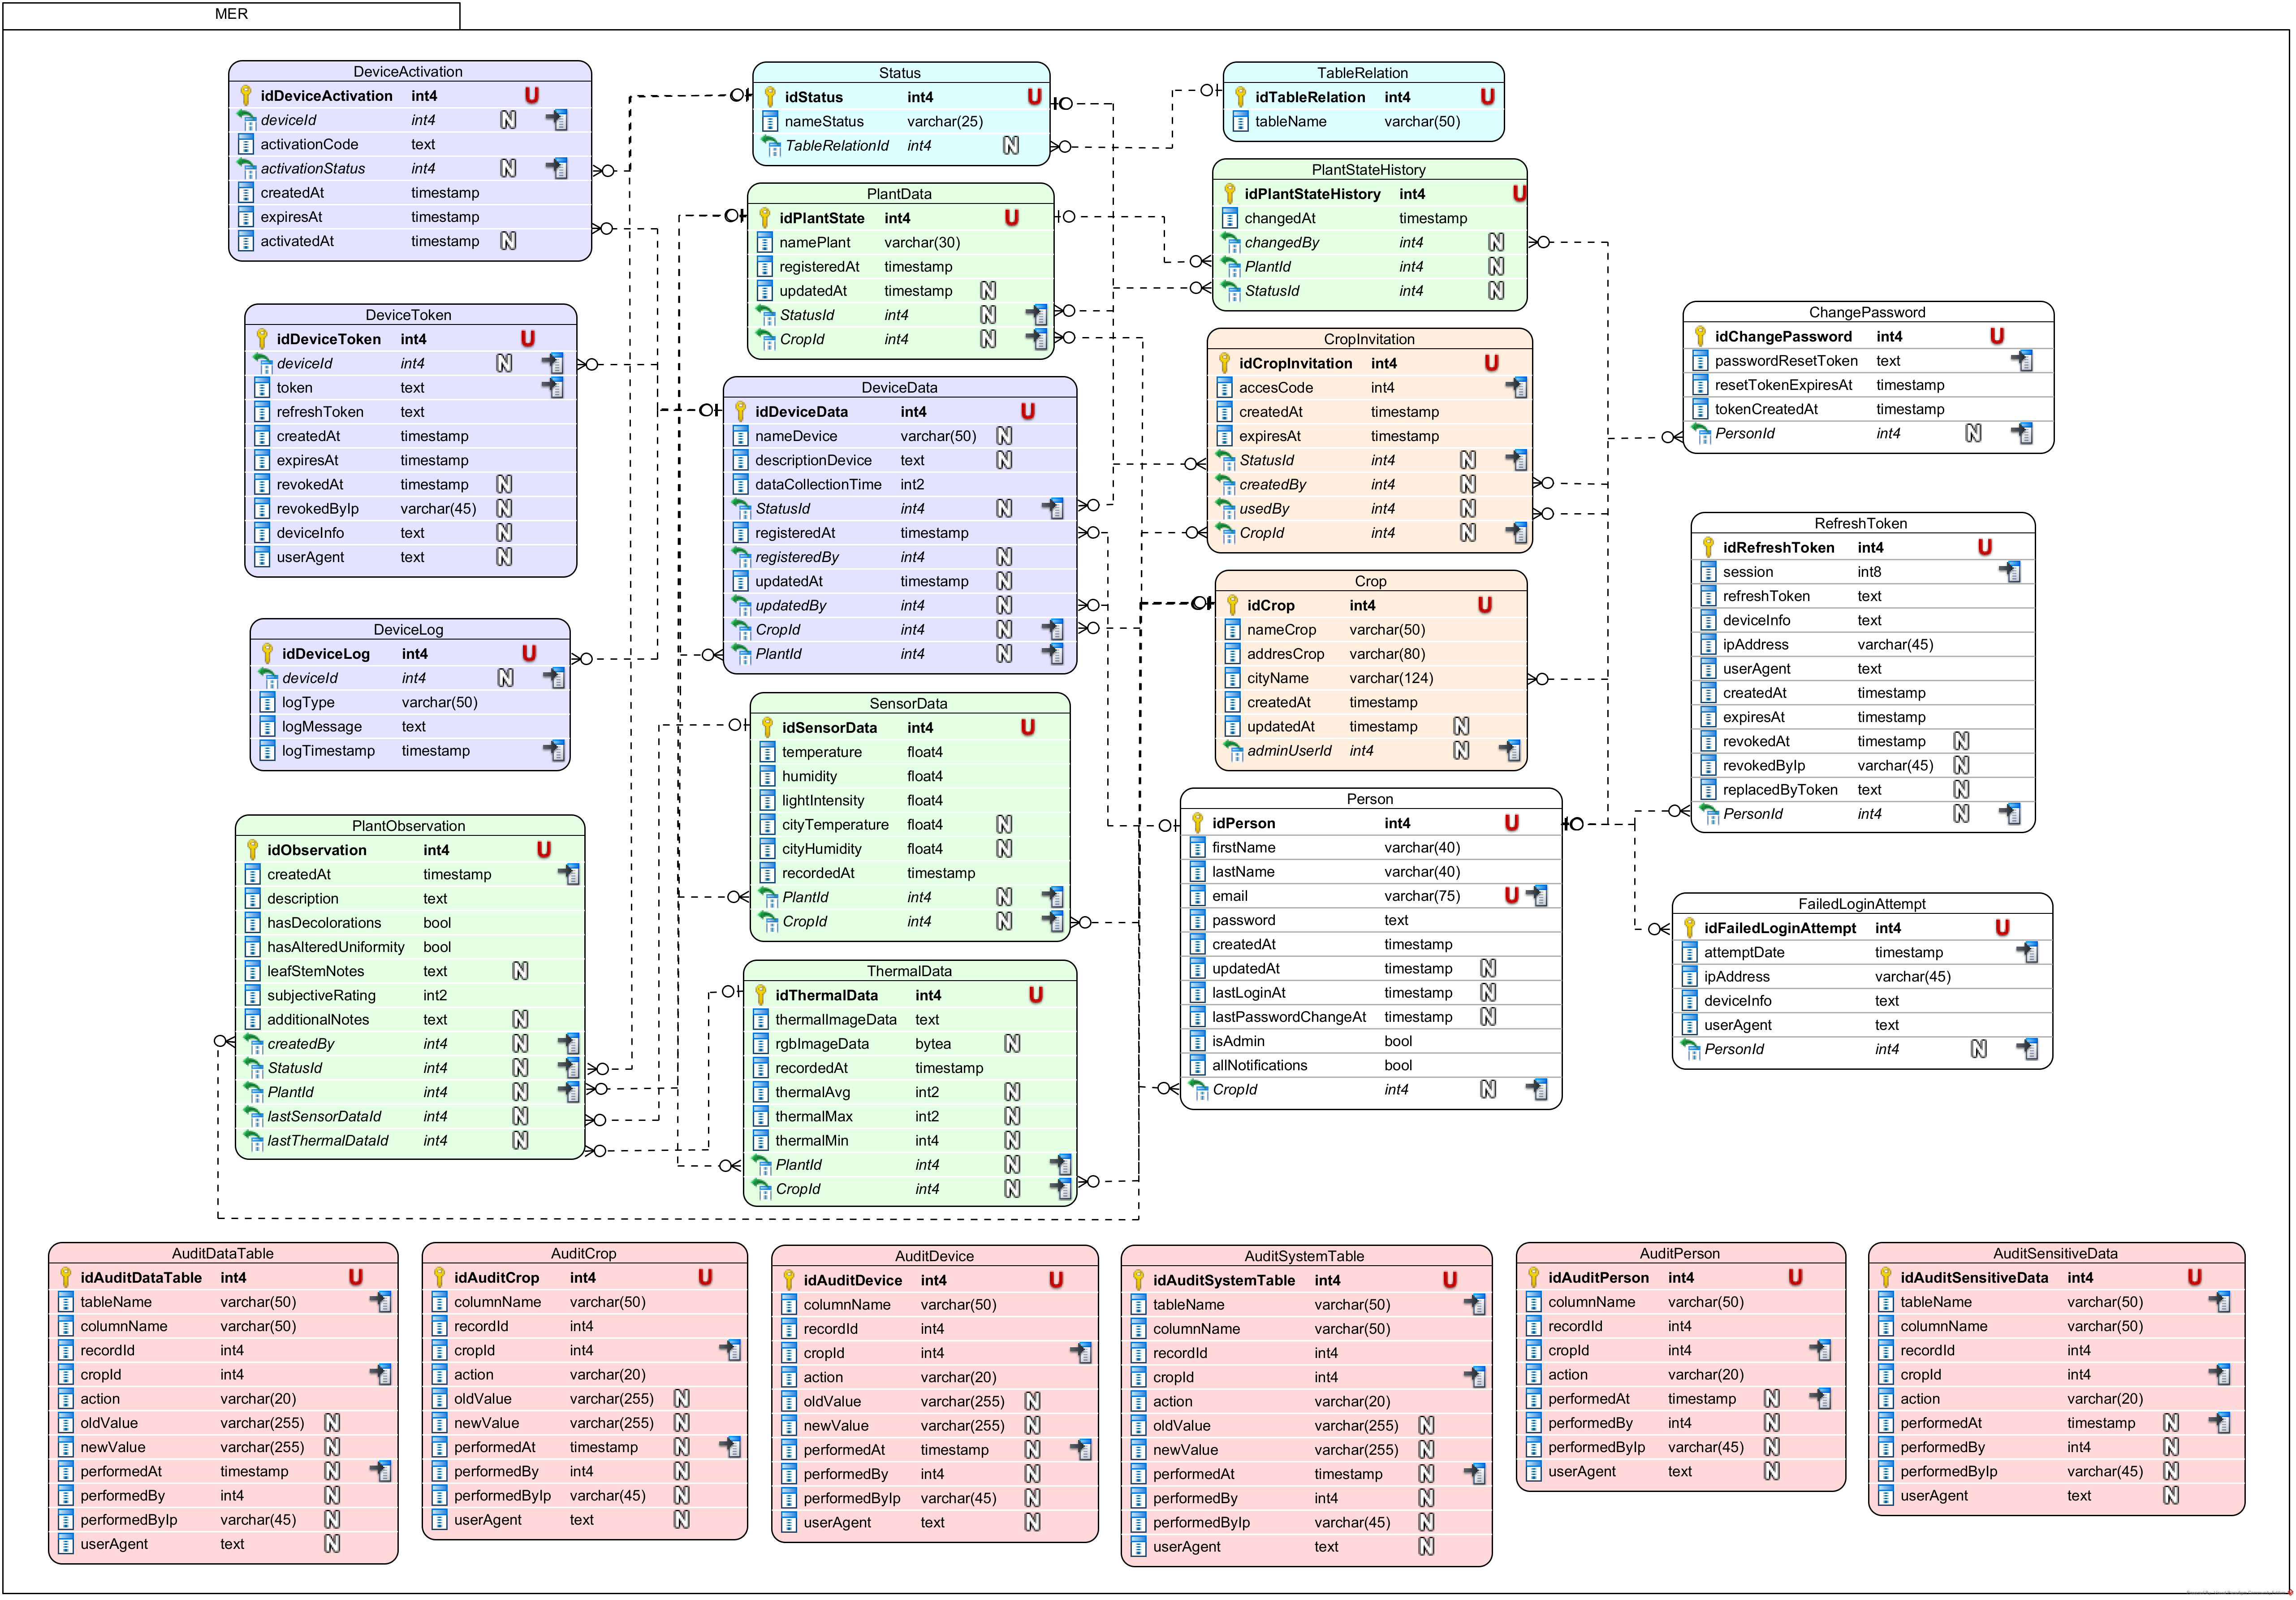
\includegraphics[width=1\textwidth]{UML/Otros/Diagrama Entidad Relacion.png}
\end{figure}

% =================================================
% =================================================

\subsection{Diagramas de Casos de Uso}

\begin{figure}[H]
    \centering
    \caption{Diagrama de Casos de Uso para la Gestión de Usuarios (RF1, RF2).}
    \label{fig:casos-uso-usuarios} % Opcional: Etiqueta para referencias
    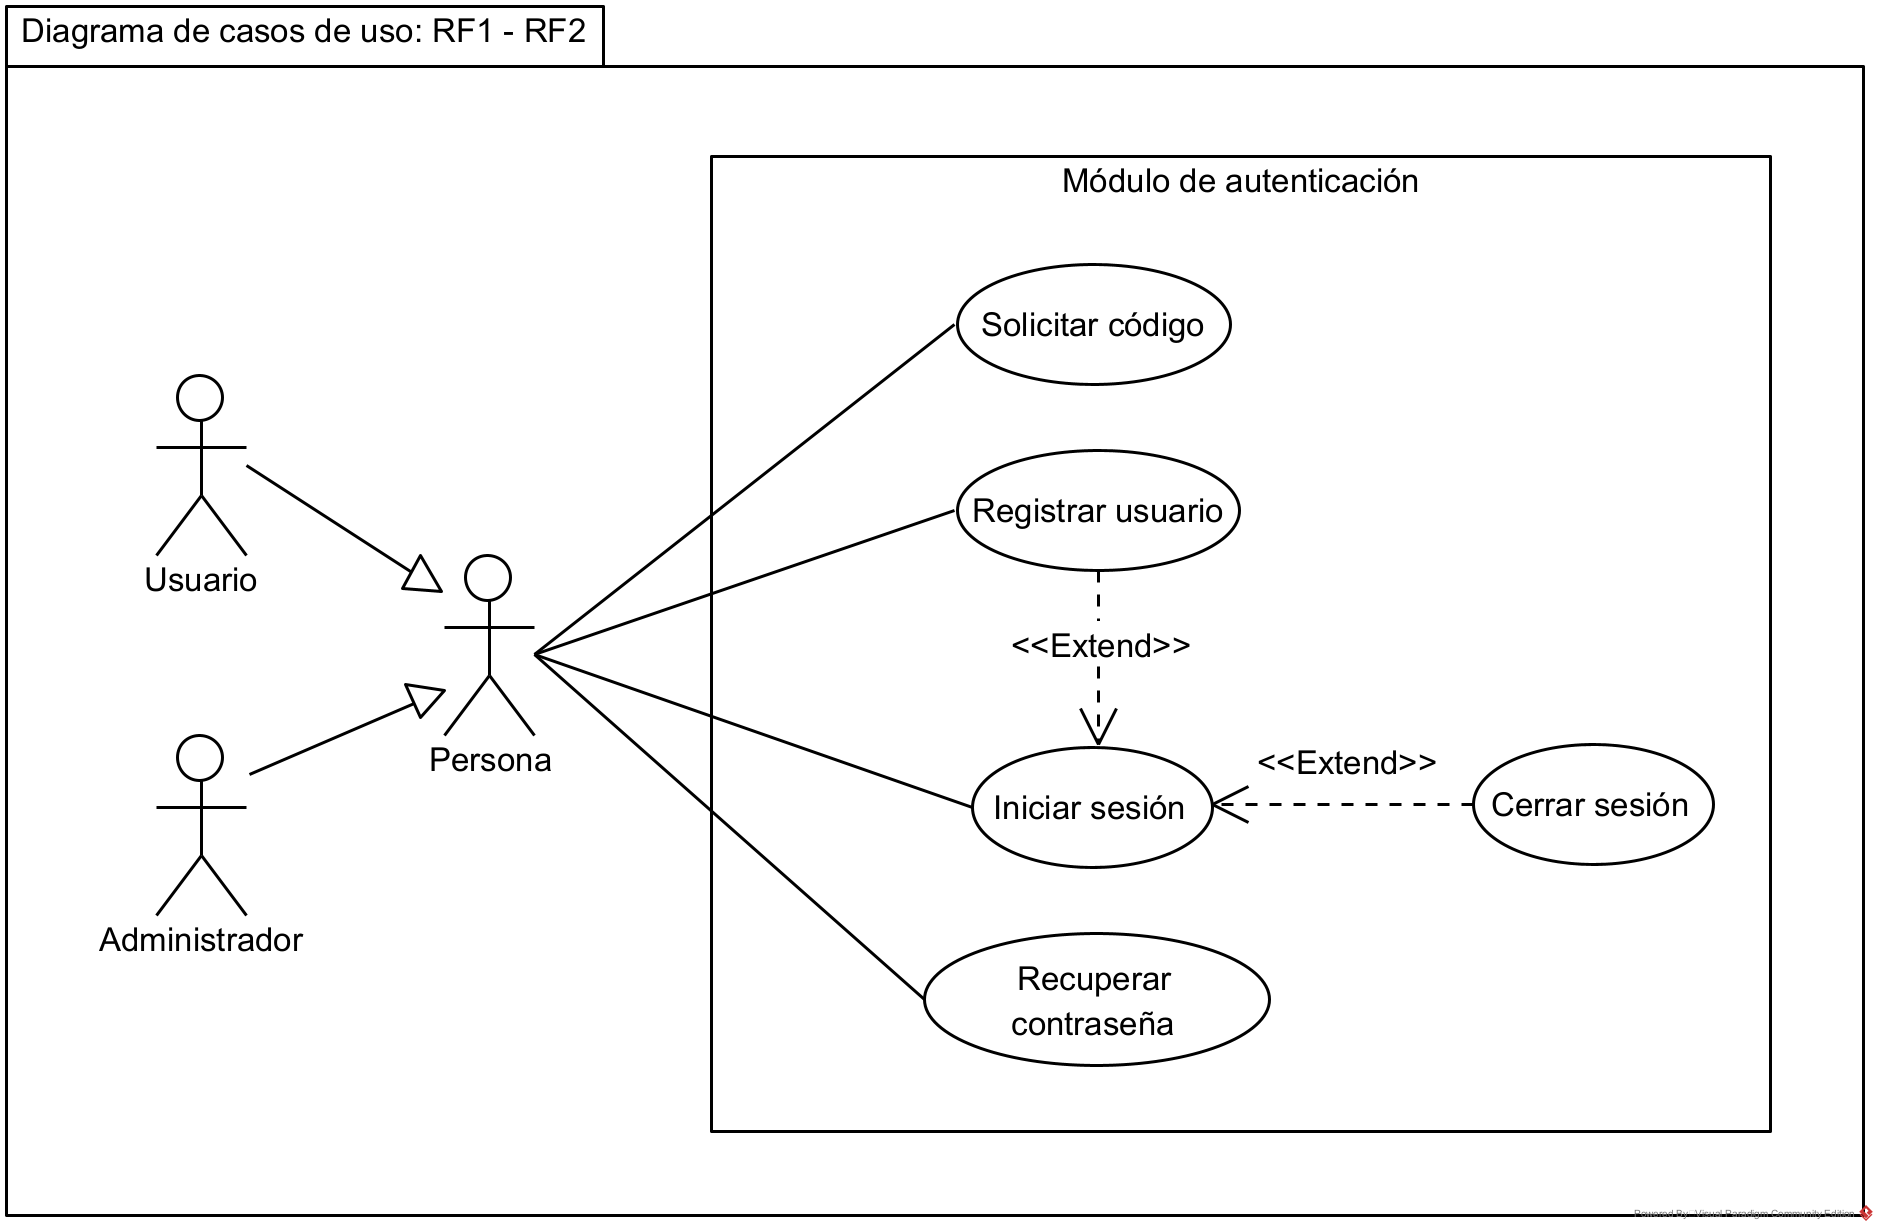
\includegraphics[width=0.8\textwidth]{UML/CasosUso/Diagrama de Casos de Uso RF1 RF2.png}
\end{figure}


\begin{figure}[H]
    \centering
    \caption{Diagrama de Casos de Uso para la Gestión de Cámaras (RF3).}
    \label{fig:casos-uso-camaras}
     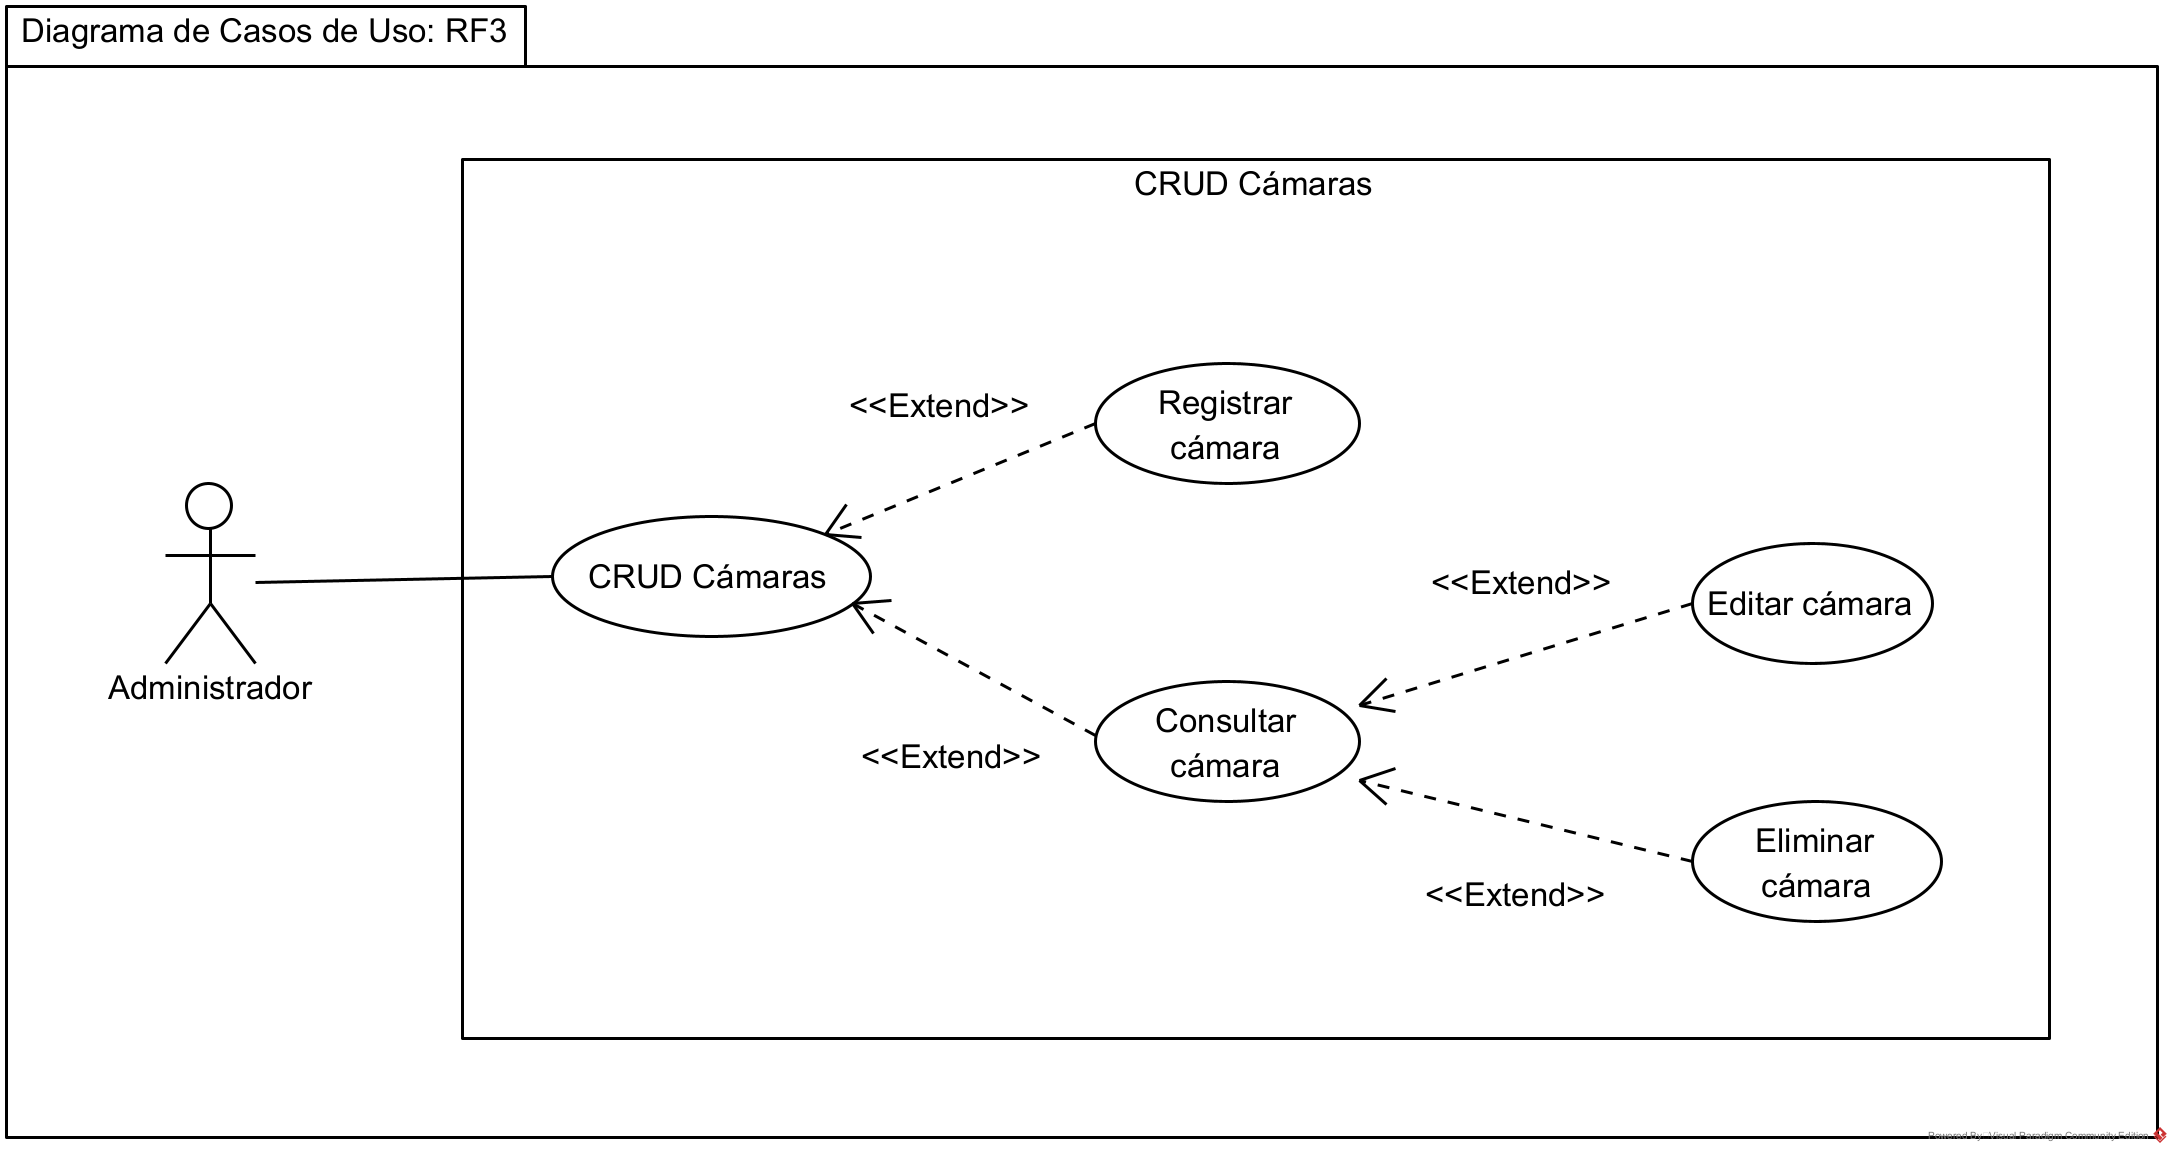
\includegraphics[width=0.8\textwidth]{UML/CasosUso/Diagrama de Casos de Uso RF3.png}
\end{figure}


\begin{figure}[H]
    \centering
    \caption{Diagrama de Casos de Uso para la Gestión de Perfiles (RF4).}
    \label{fig:casos-uso-perfiles}
    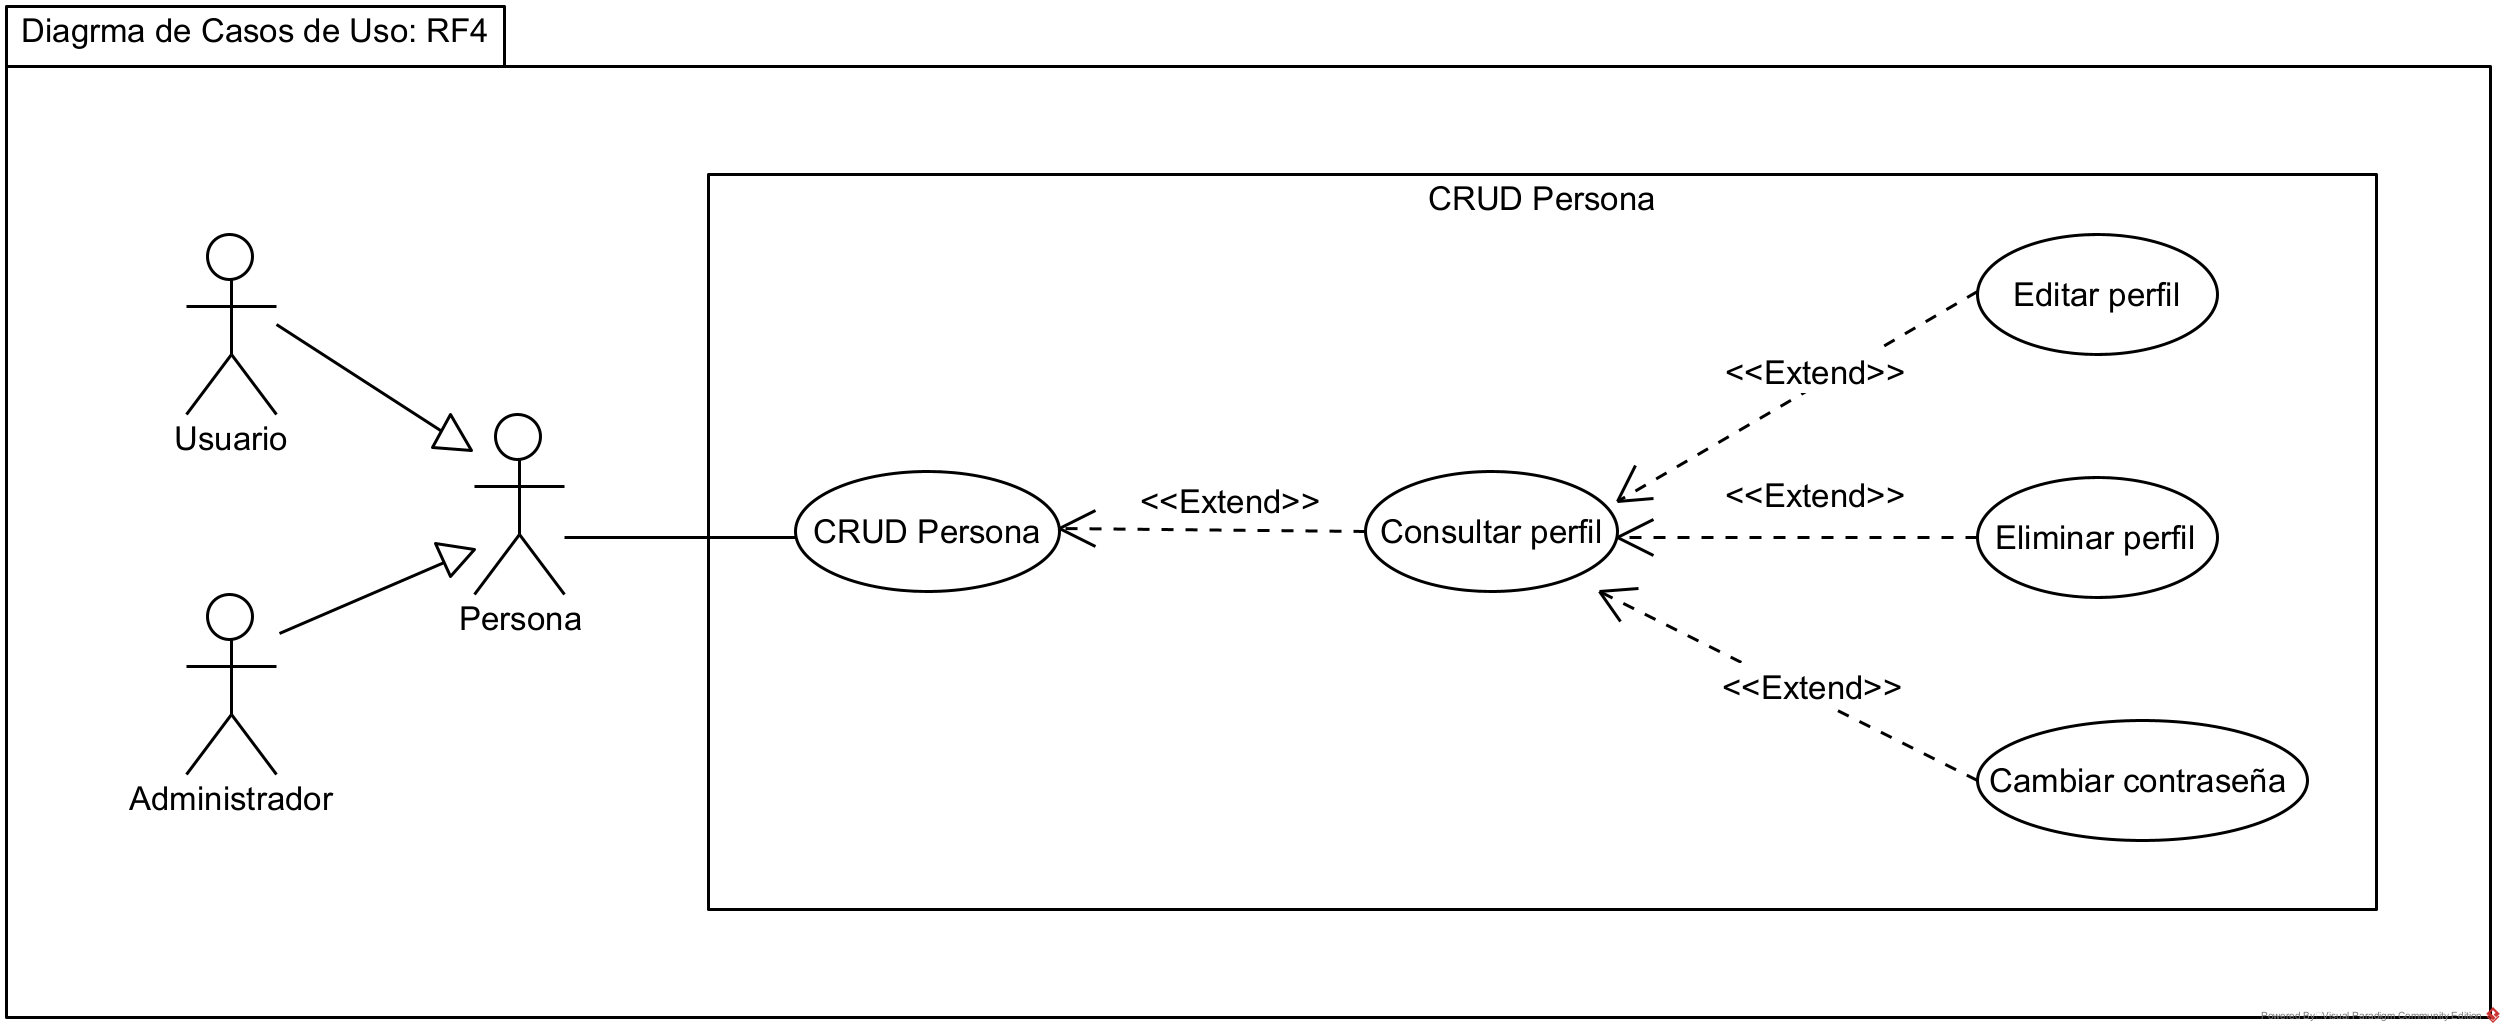
\includegraphics[width=0.8\textwidth]{UML/CasosUso/Diagrama de Casos de Uso RF4.png}
\end{figure}


\begin{figure}[H]
    \centering
    \caption{Diagrama de Casos de Uso para el Módulo de Mediciones (RF5).}
    \label{fig:casos-uso-mediciones}
    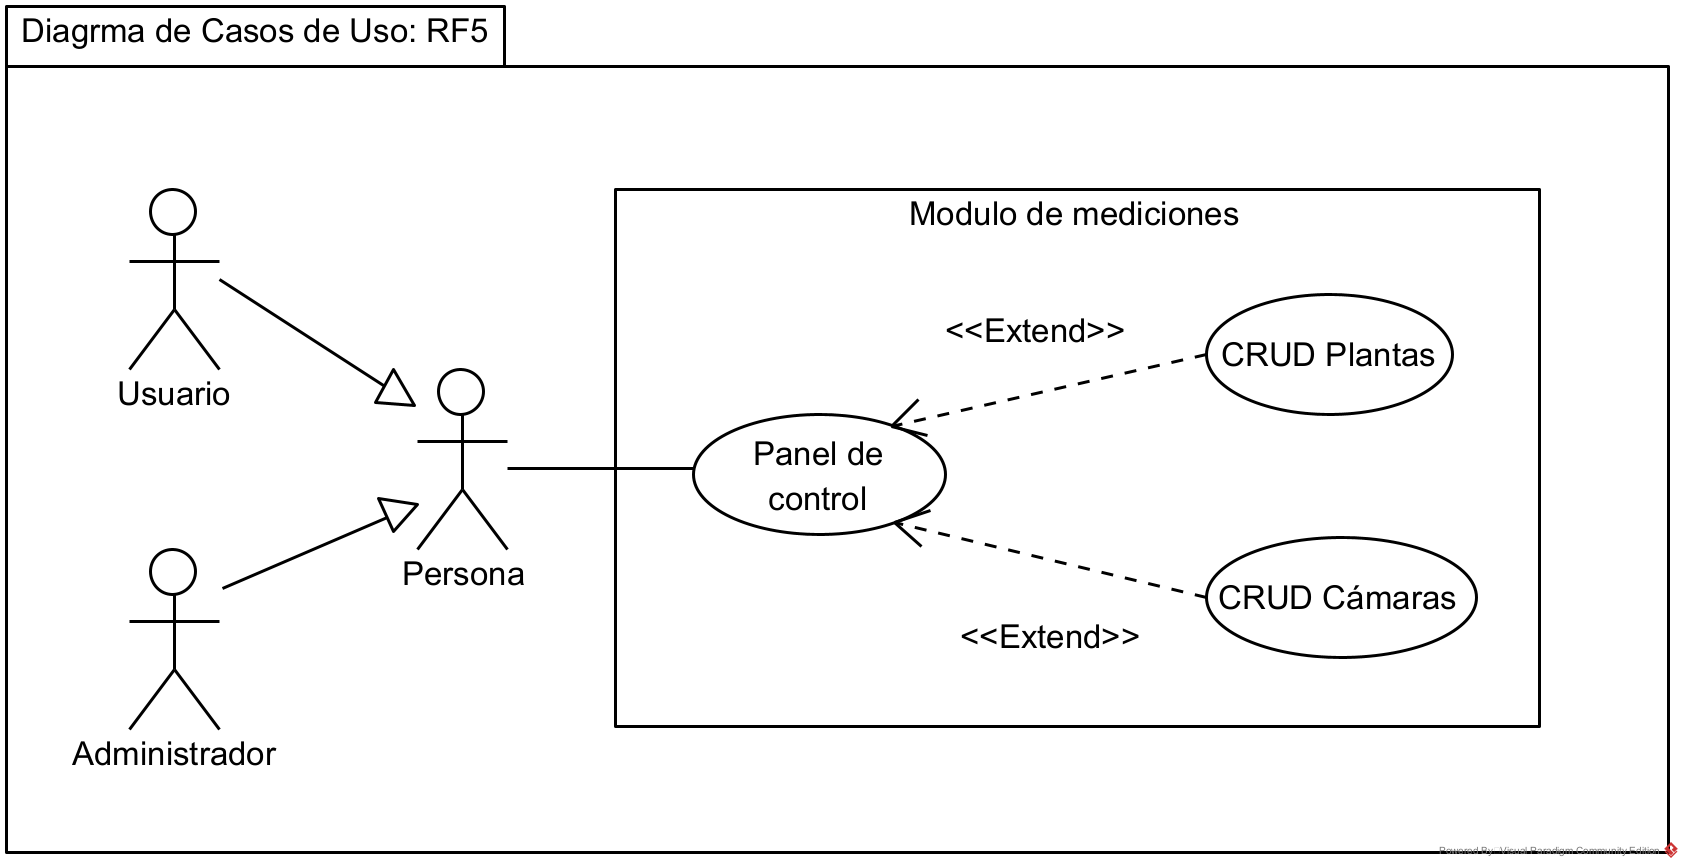
\includegraphics[width=0.8\textwidth]{UML/CasosUso/Diagrama de Casos de Uso RF5.png}
\end{figure}


\begin{figure}[H]
    \centering
    \caption{Diagrama de Casos de Uso para la Gestión de Plantas (RF6).}
    \label{fig:casos-uso-plantas}
    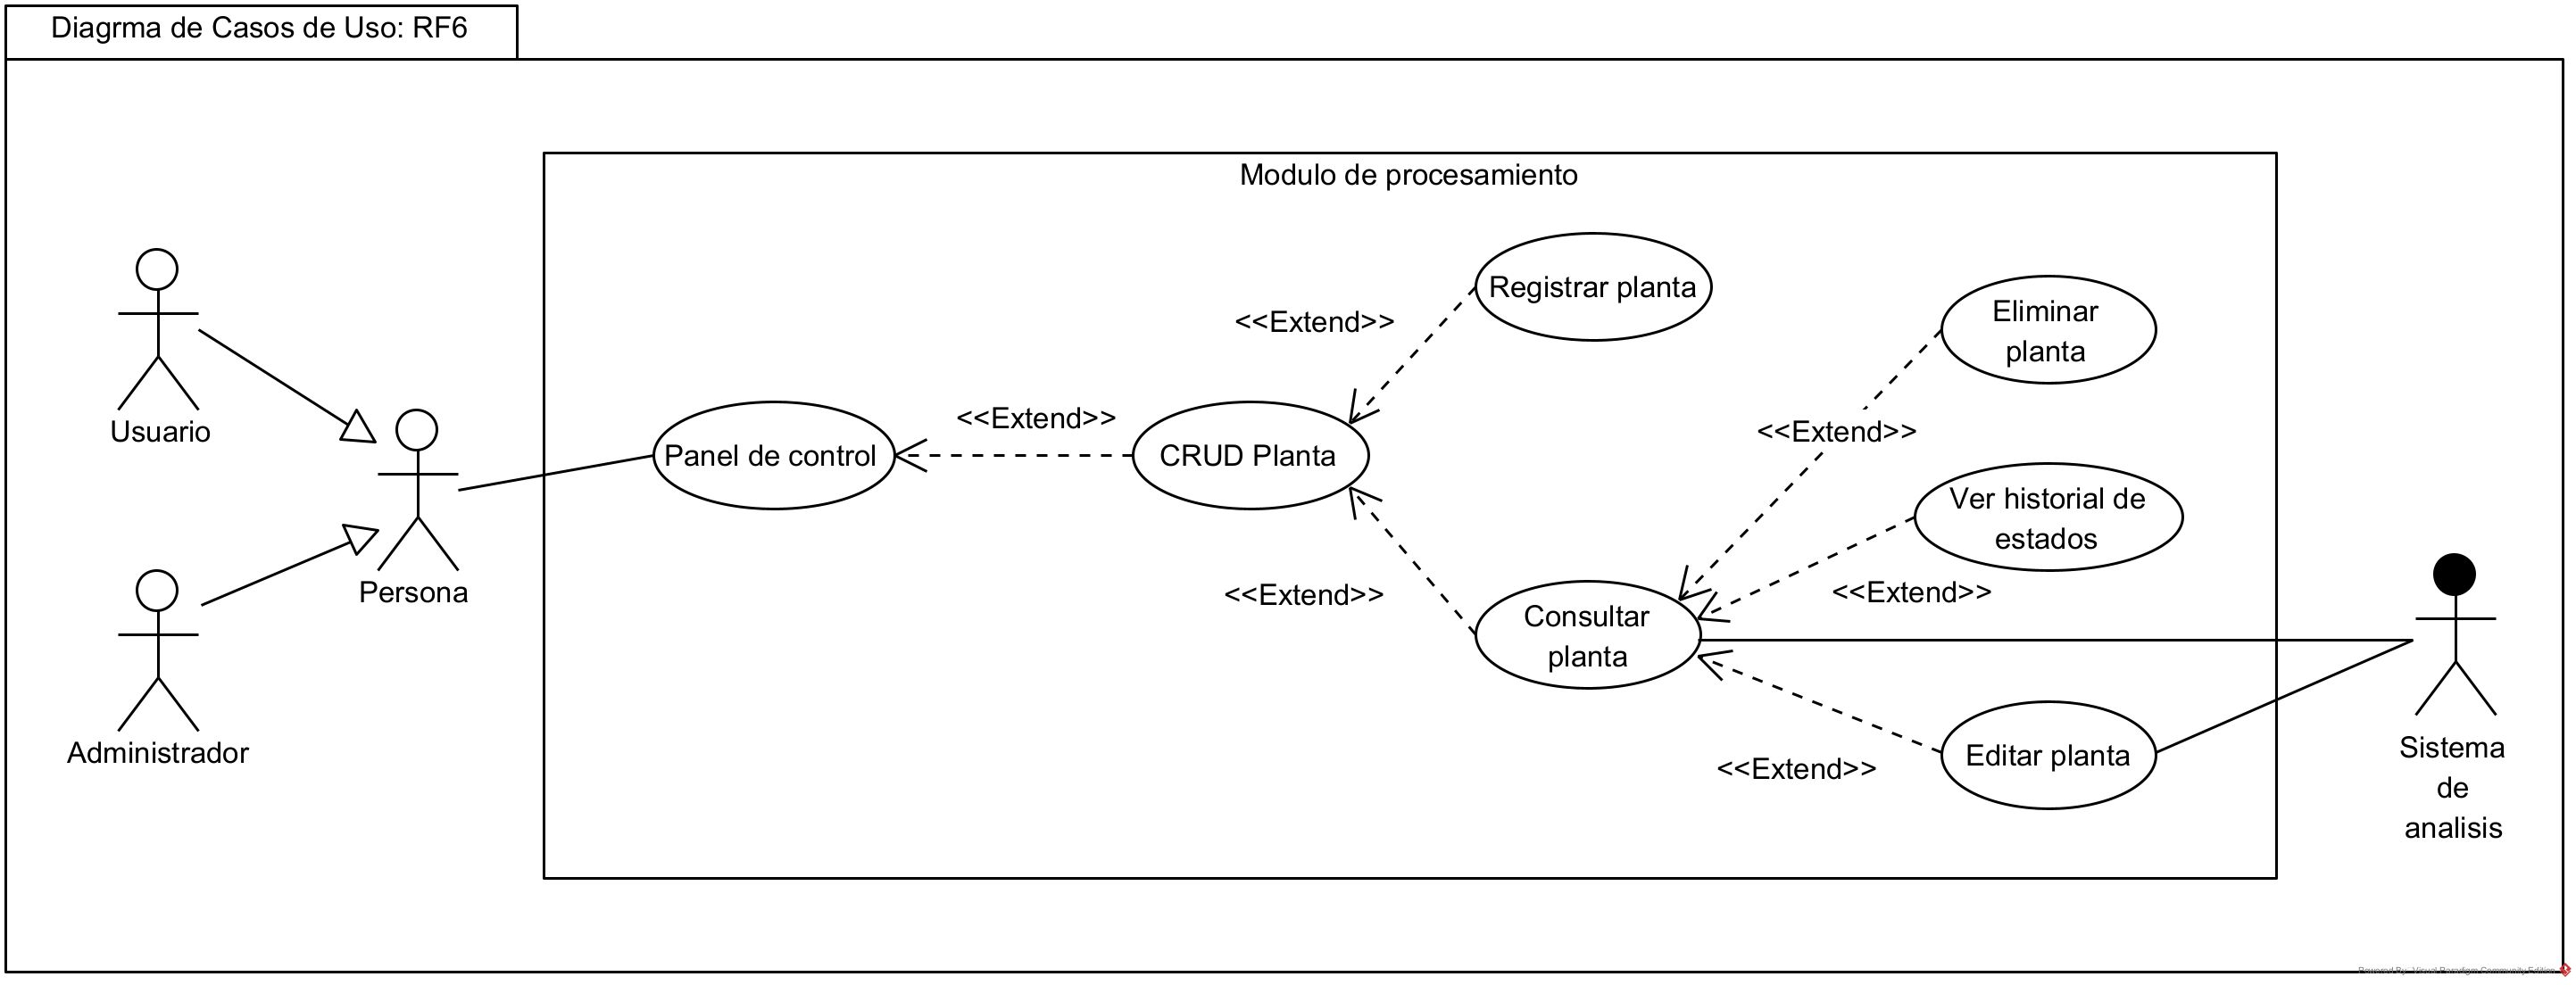
\includegraphics[width=0.8\textwidth]{UML/CasosUso/Diagrama de Casos de Uso RF6.png}
\end{figure}


\begin{figure}[H]
    \centering
    \caption{Diagrama de Casos de Uso para la Generación de Reportes (RF7).}
    \label{fig:casos-uso-reportes}
     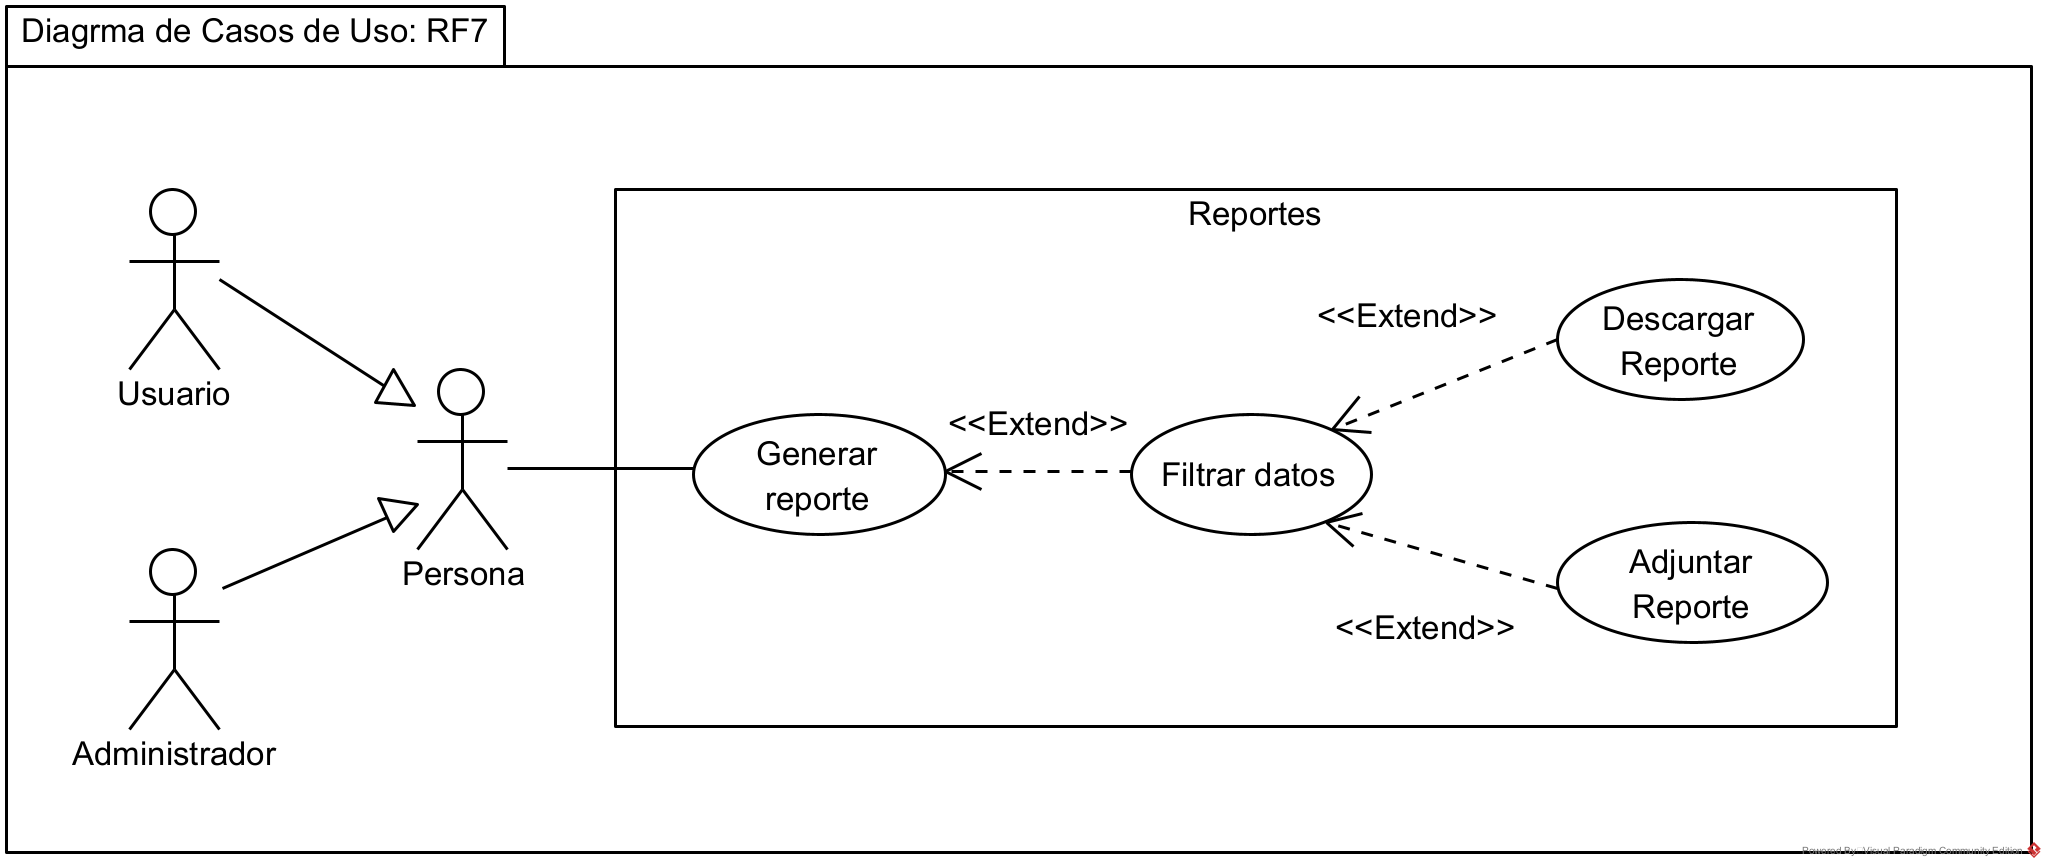
\includegraphics[width=0.8\textwidth]{UML/CasosUso/Diagrama de Casos de Uso RF7.png}
\end{figure}


\begin{figure}[H]
    \centering
    \caption{Diagrama de Casos de Uso para las Notificaciones (RF8).}
    \label{fig:casos-uso-notificaciones}
    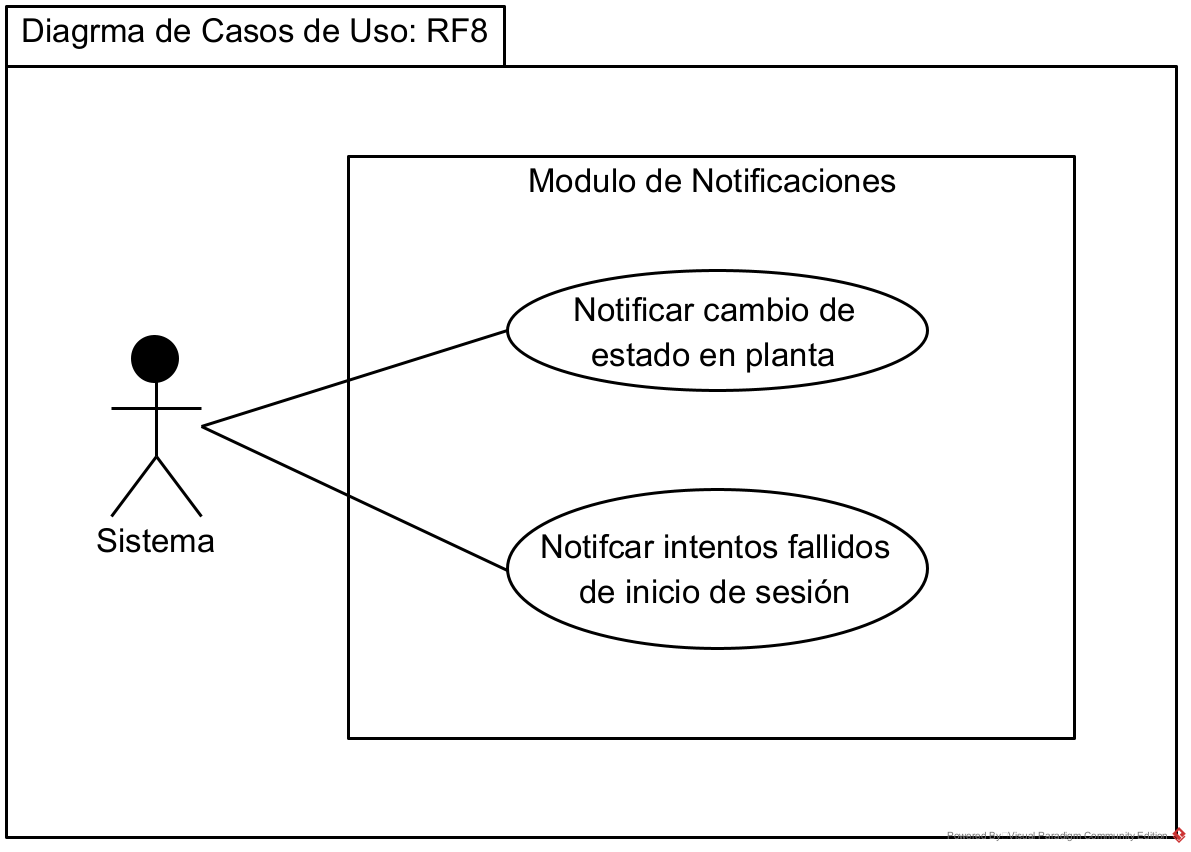
\includegraphics[width=0.8\textwidth]{UML/CasosUso/Diagrama de Casos de Uso RF8.png}
\end{figure}


\begin{figure}[H]
    \centering
    \caption{Diagrama de Casos de Uso para el Módulo de Observaciones (RF9).}
    \label{fig:casos-uso-observaciones}
    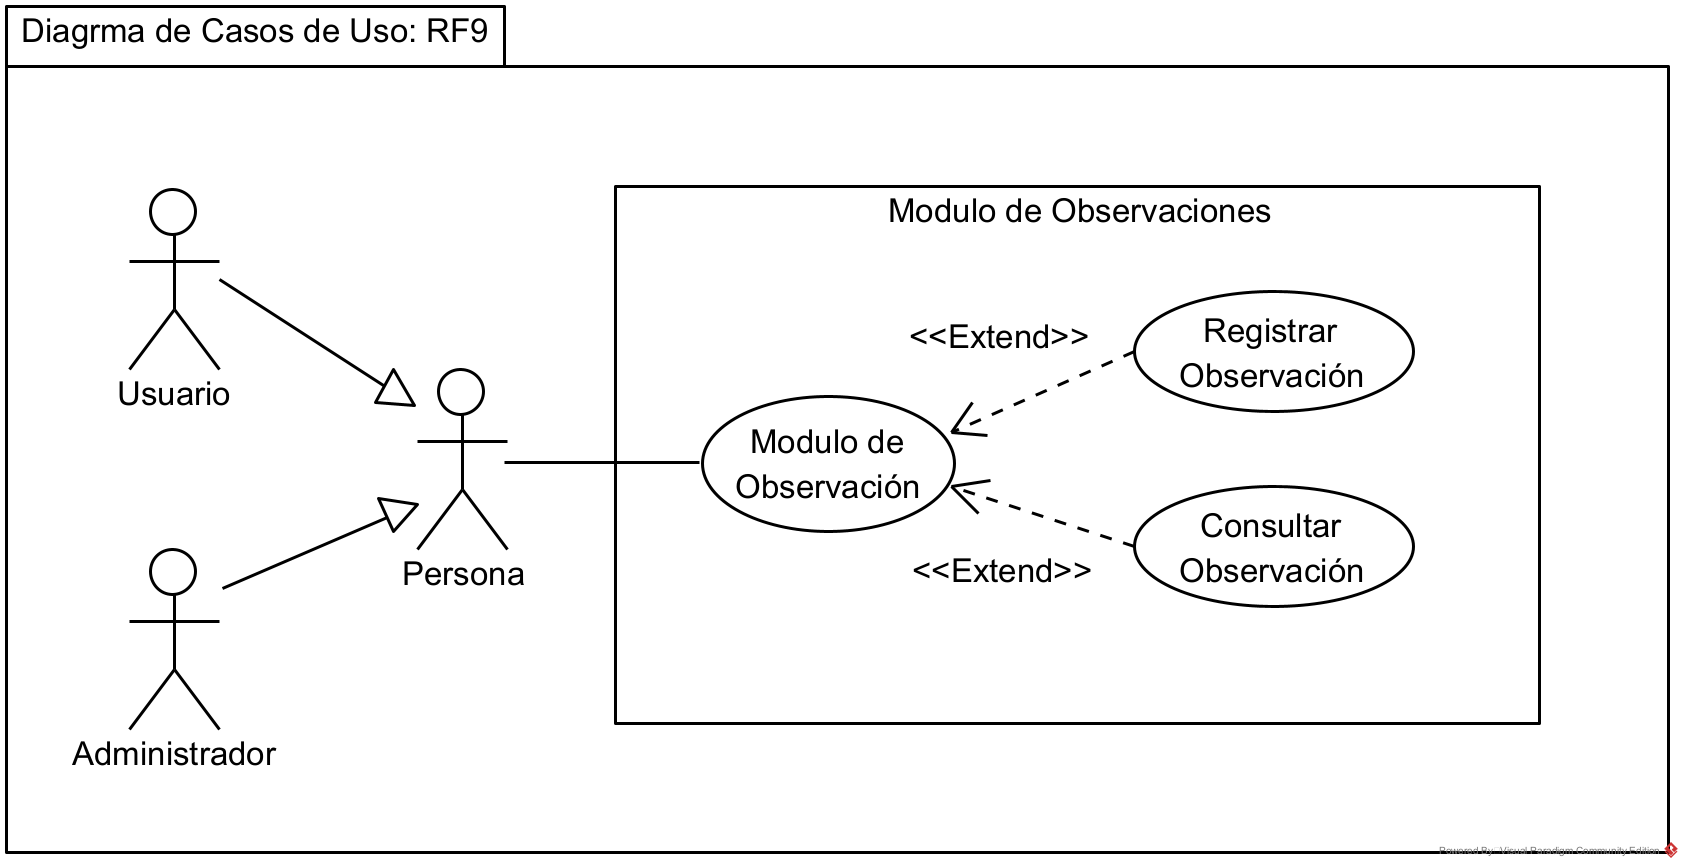
\includegraphics[width=0.8\textwidth]{UML/CasosUso/Diagrama de Casos de Uso RF9.png}
\end{figure}

% =================================================
% =================================================

\subsection{Diagramas de Secuencia}


\begin{figure}[H]
    \centering
    \caption{Diagrama de secuencia base: Envío de formulario.}
    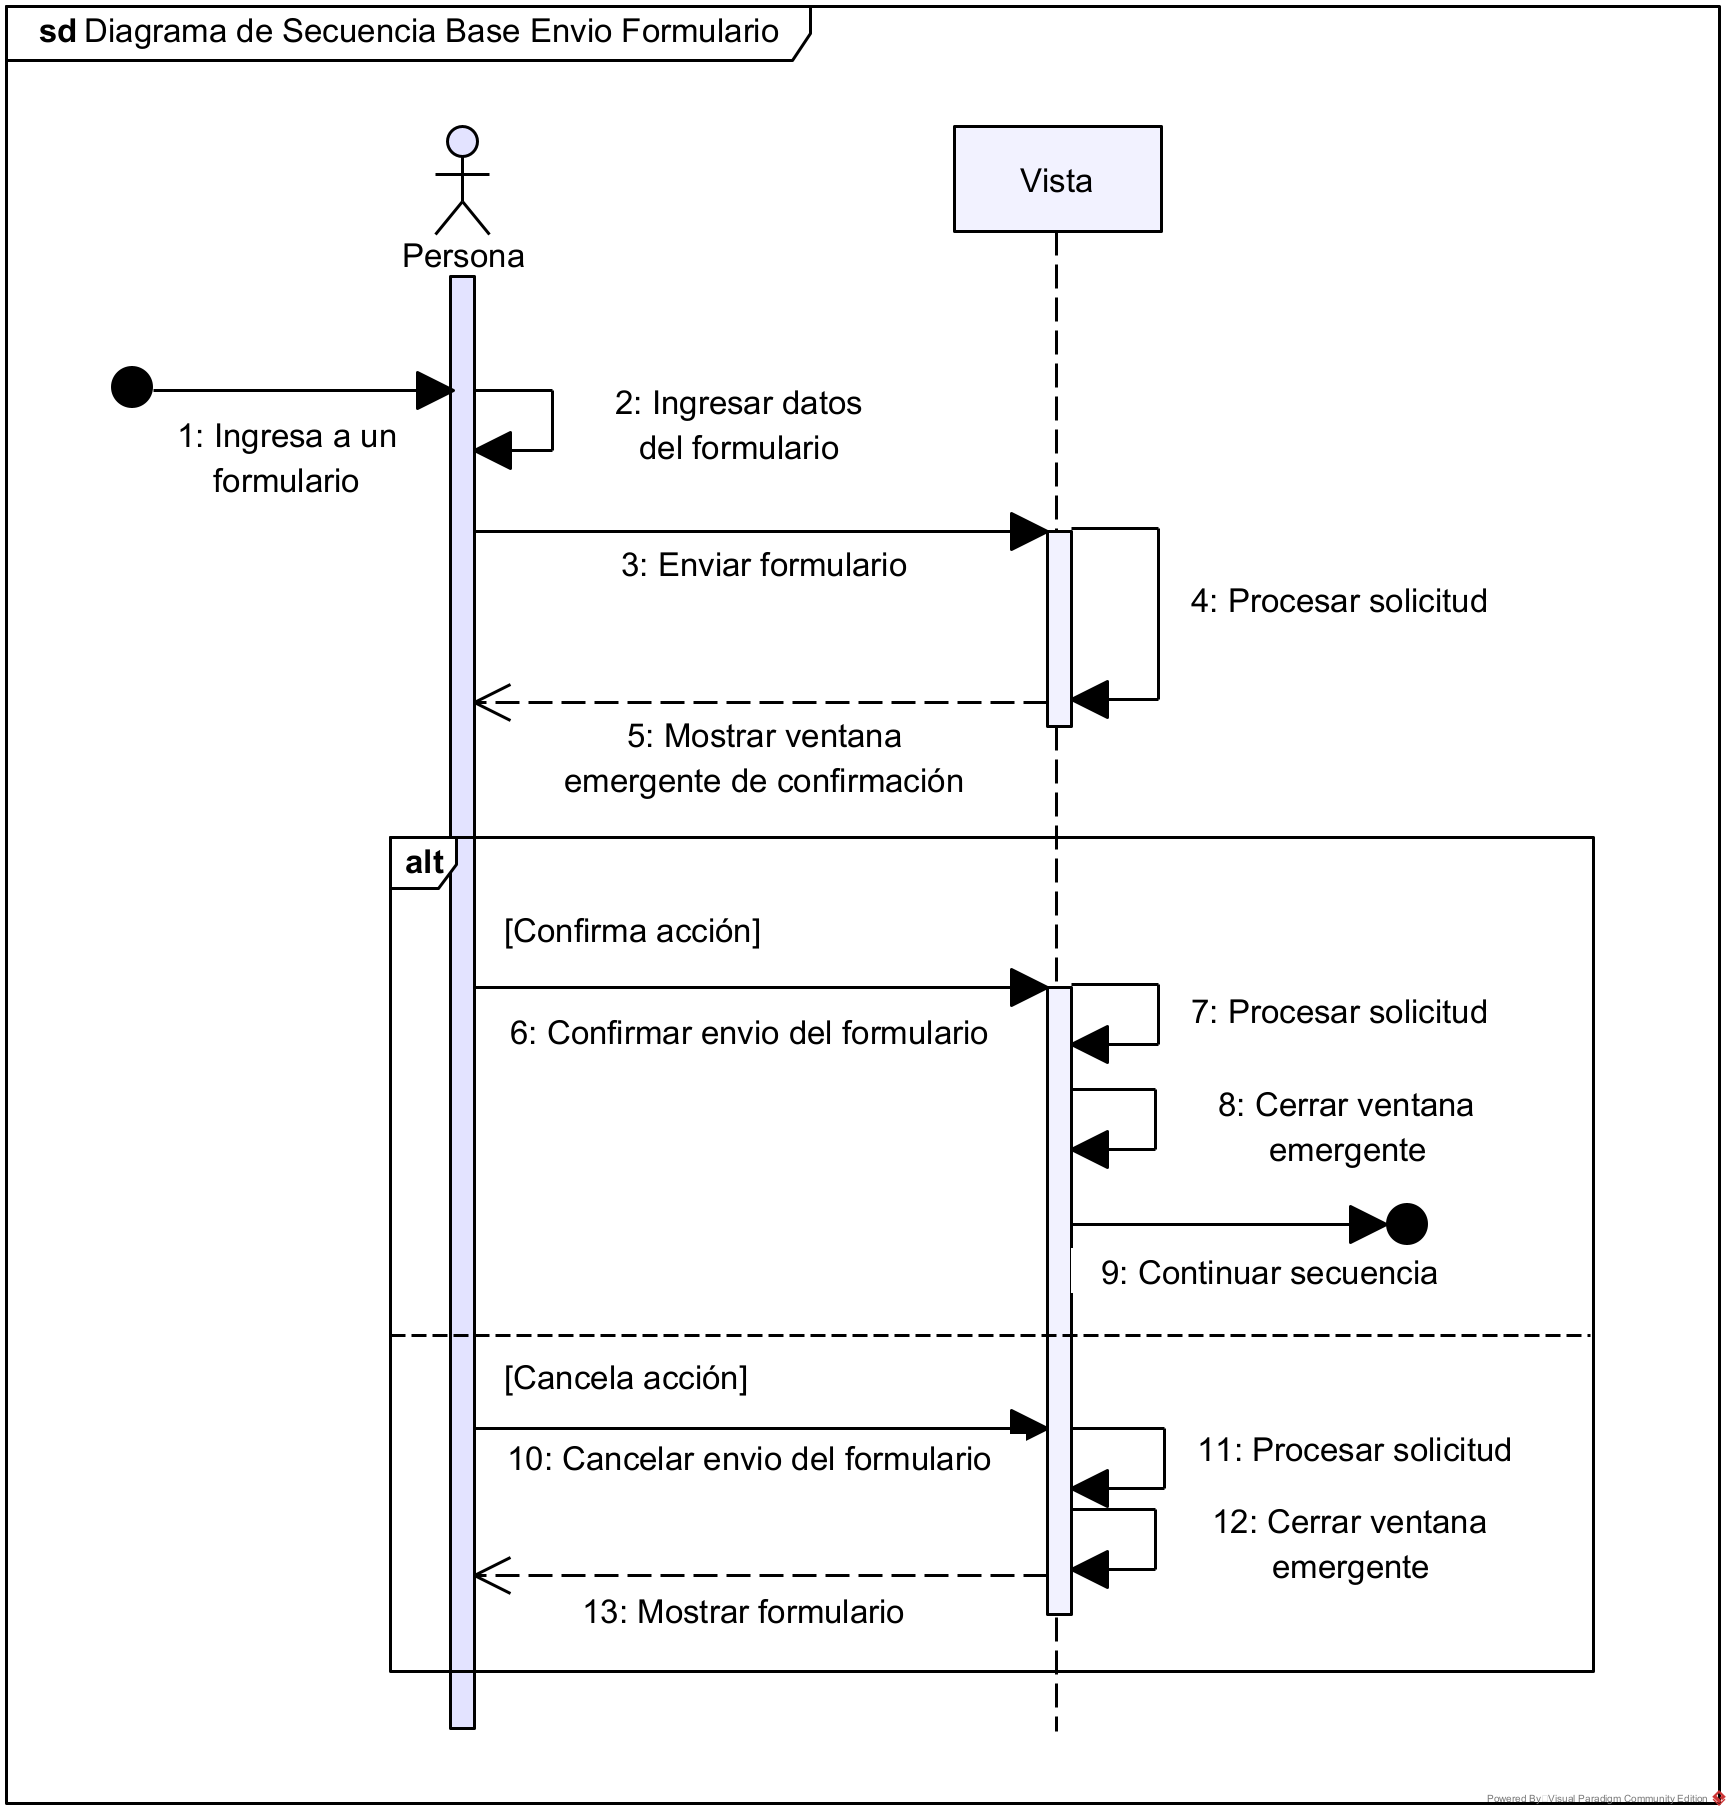
\includegraphics[width=0.8\textwidth]{UML/Secuencia/Diagrama de Secuencia Base Envio Formulario.png}
\end{figure}


\begin{figure}[H]
    \centering
    \caption{Diagrama de Secuencia para el Registro (RF1.0).}
 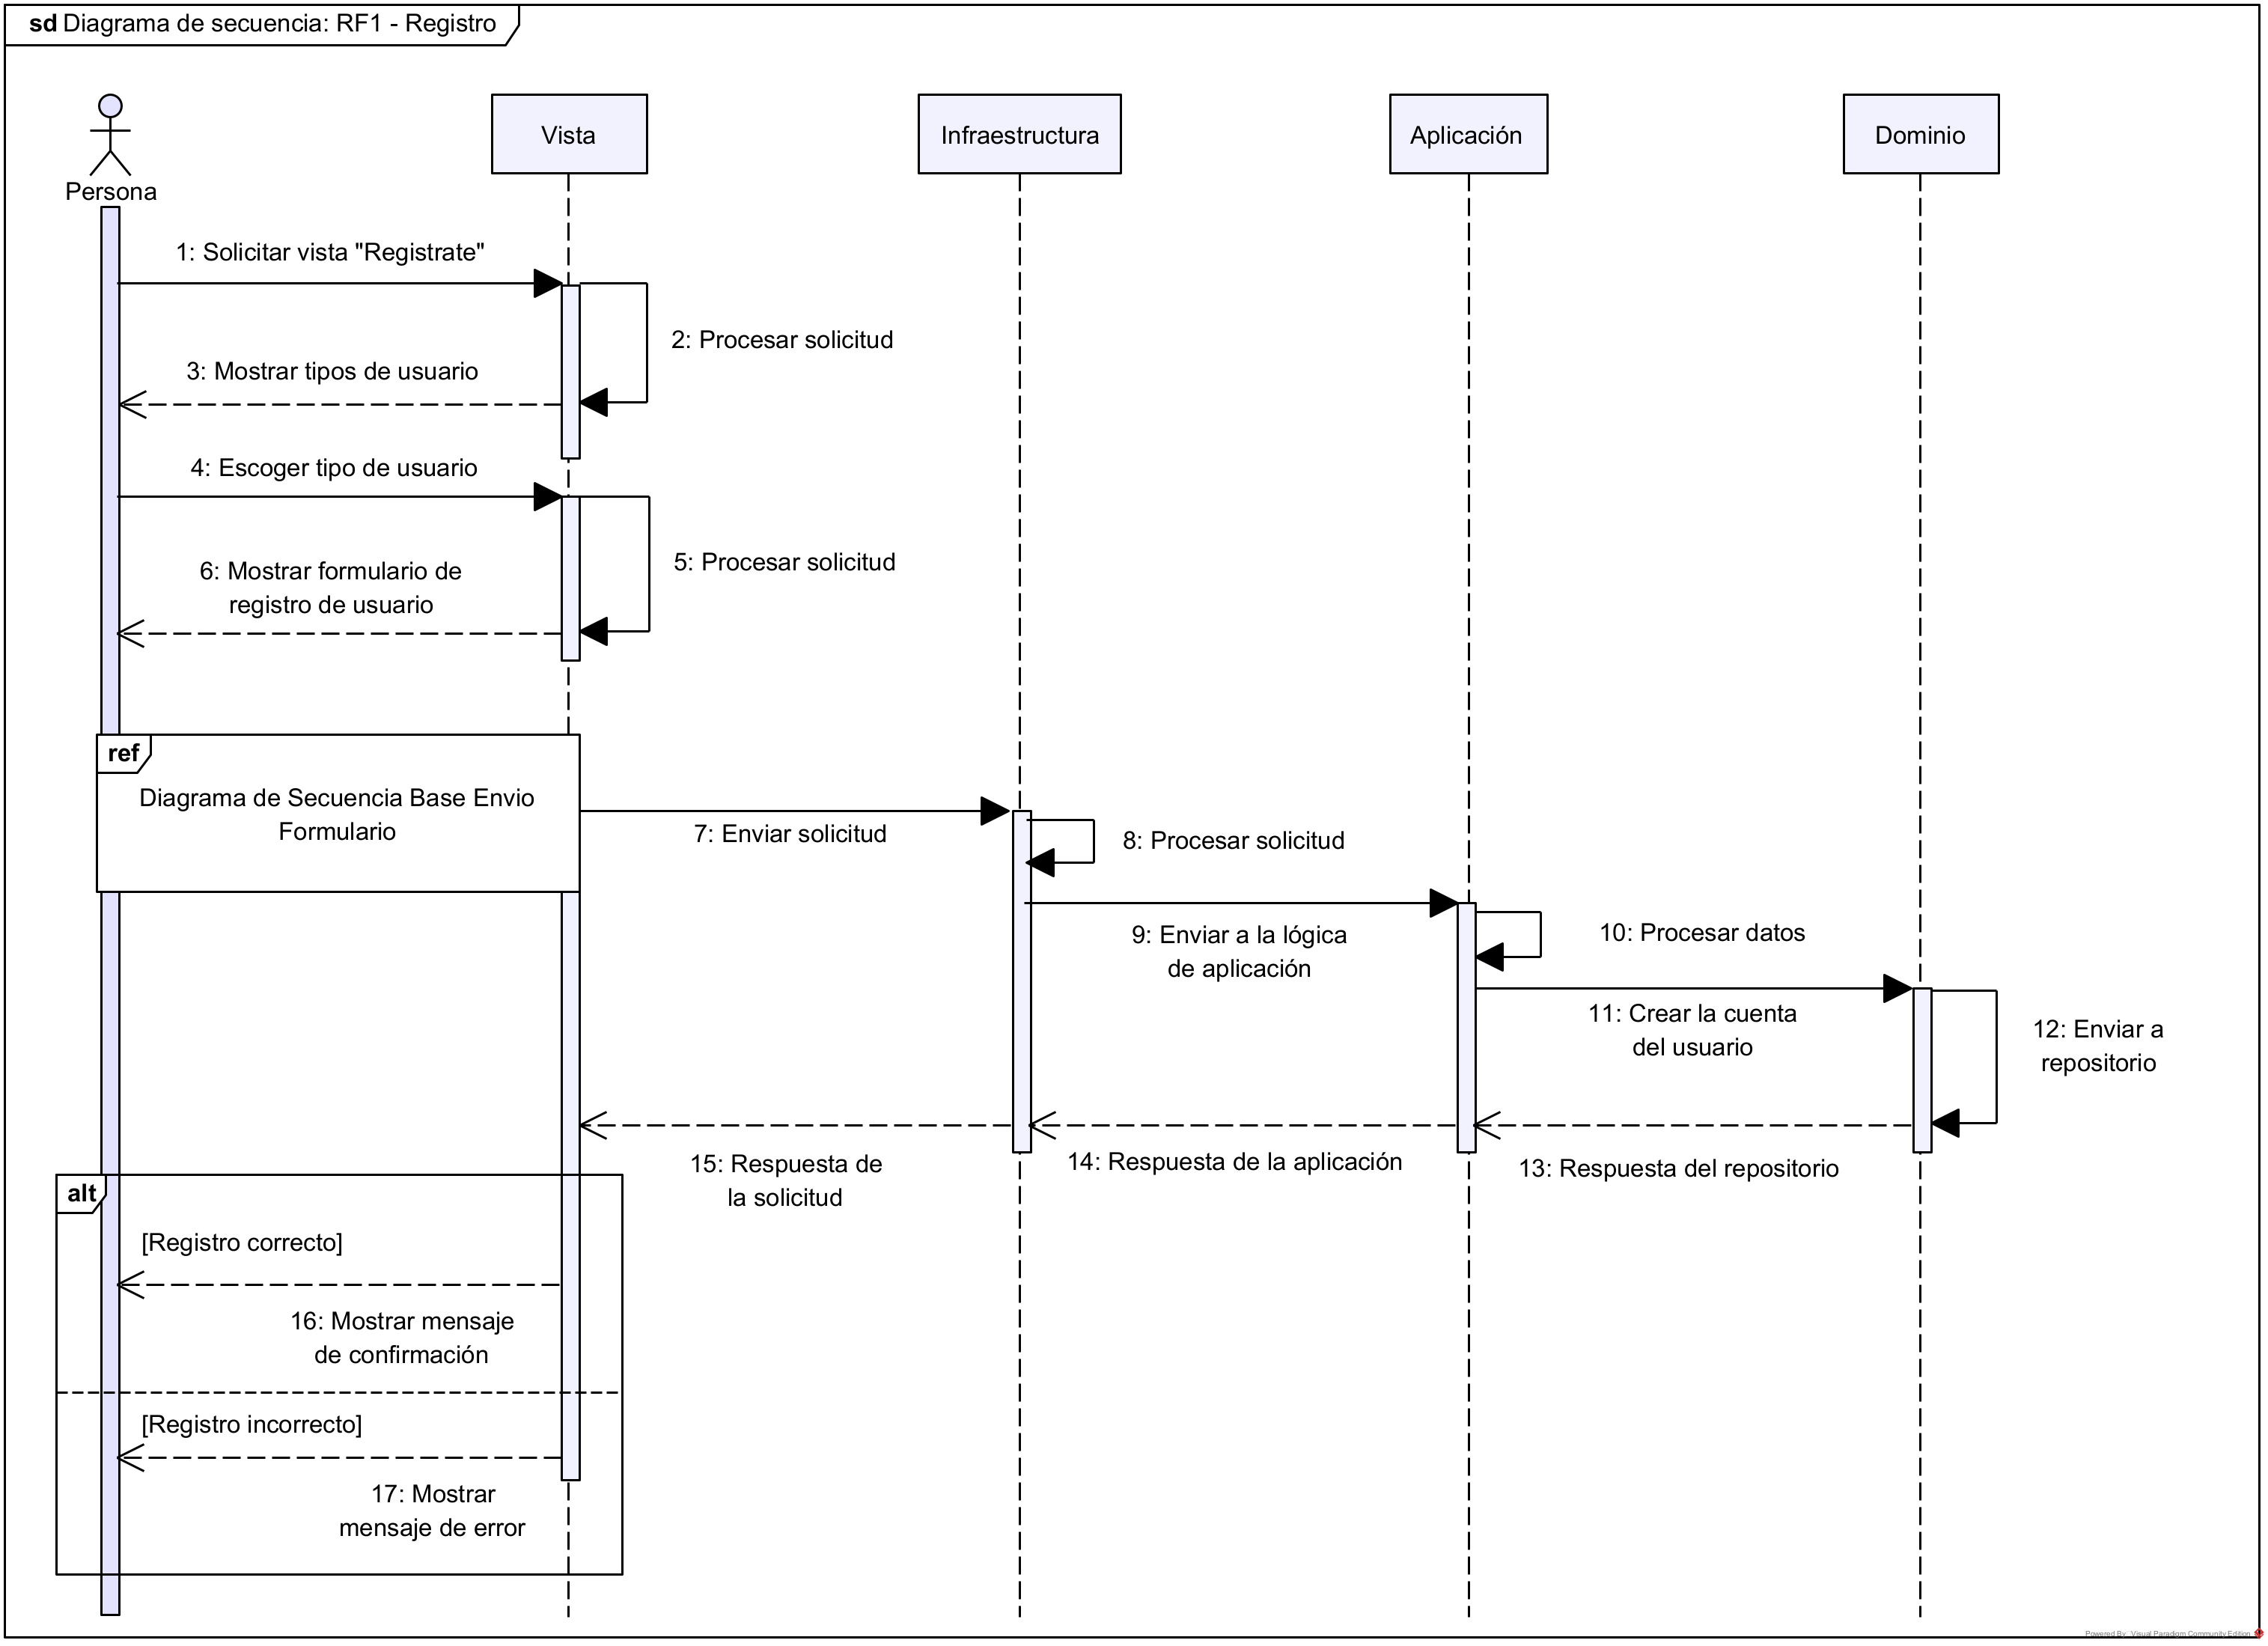
\includegraphics[width=0.8\textwidth]{UML/Secuencia/Diagrama de Secuencia RF1.0 Registro.png}
\end{figure}


\begin{figure}[H]
    \centering
    \caption{Diagrama de Secuencia para Solicitar Código (RF1.1).}
    \includegraphics[width=0.8\textwidth]{UML/Secuencia/Diagrama de Secuencia RF1.1 Solicitar Código.png}
\end{figure}


\begin{figure}[H]
	\centering
	\caption{Diagrama de Secuencia para Iniciar Sesión (RF2.0).}
	\includegraphics[width=0.8\textwidth]{UML/Secuencia/Diagrama de Secuencia RF2.0 Iniciar Sesión.png}
\end{figure}


\begin{figure}[H]
	\centering
	\caption{Diagrama de Secuencia para Cerrar Sesión (RF2.1).}
 \includegraphics[width=0.8\textwidth]{UML/Secuencia/Diagrama de Secuencia RF2.1 Cerrar Sesión.png}
\end{figure}


\begin{figure}[H]
	\centering
		\caption{Diagrama de Secuencia para Recuperar Contraseña (RF2.2).}
	\includegraphics[width=0.8\textwidth]{UML/Secuencia/Diagrama de Secuencia RF2.2 Recuperar Contraseña.png}
\end{figure}


\begin{figure}[H]
	\centering
		\caption{Diagrama de Secuencia para Crear Cámara (RF3.1).}
	\includegraphics[width=0.8\textwidth]{UML/Secuencia/Diagrama de Secuencia RF3.1 Crear Cámara.png}
\end{figure}


\begin{figure}[H]
	\centering
		\caption{Diagrama de Secuencia para Activar Cámara (RF3.1.1).}
	\includegraphics[width=0.63\textwidth]{UML/Secuencia/Diagrama de Secuencia RF3.1.1 Activar Cámara.png}
\end{figure}


\begin{figure}[H]
	\centering
	\caption{Diagrama de Secuencia para Activar Hardware (RF3.1.1).}
	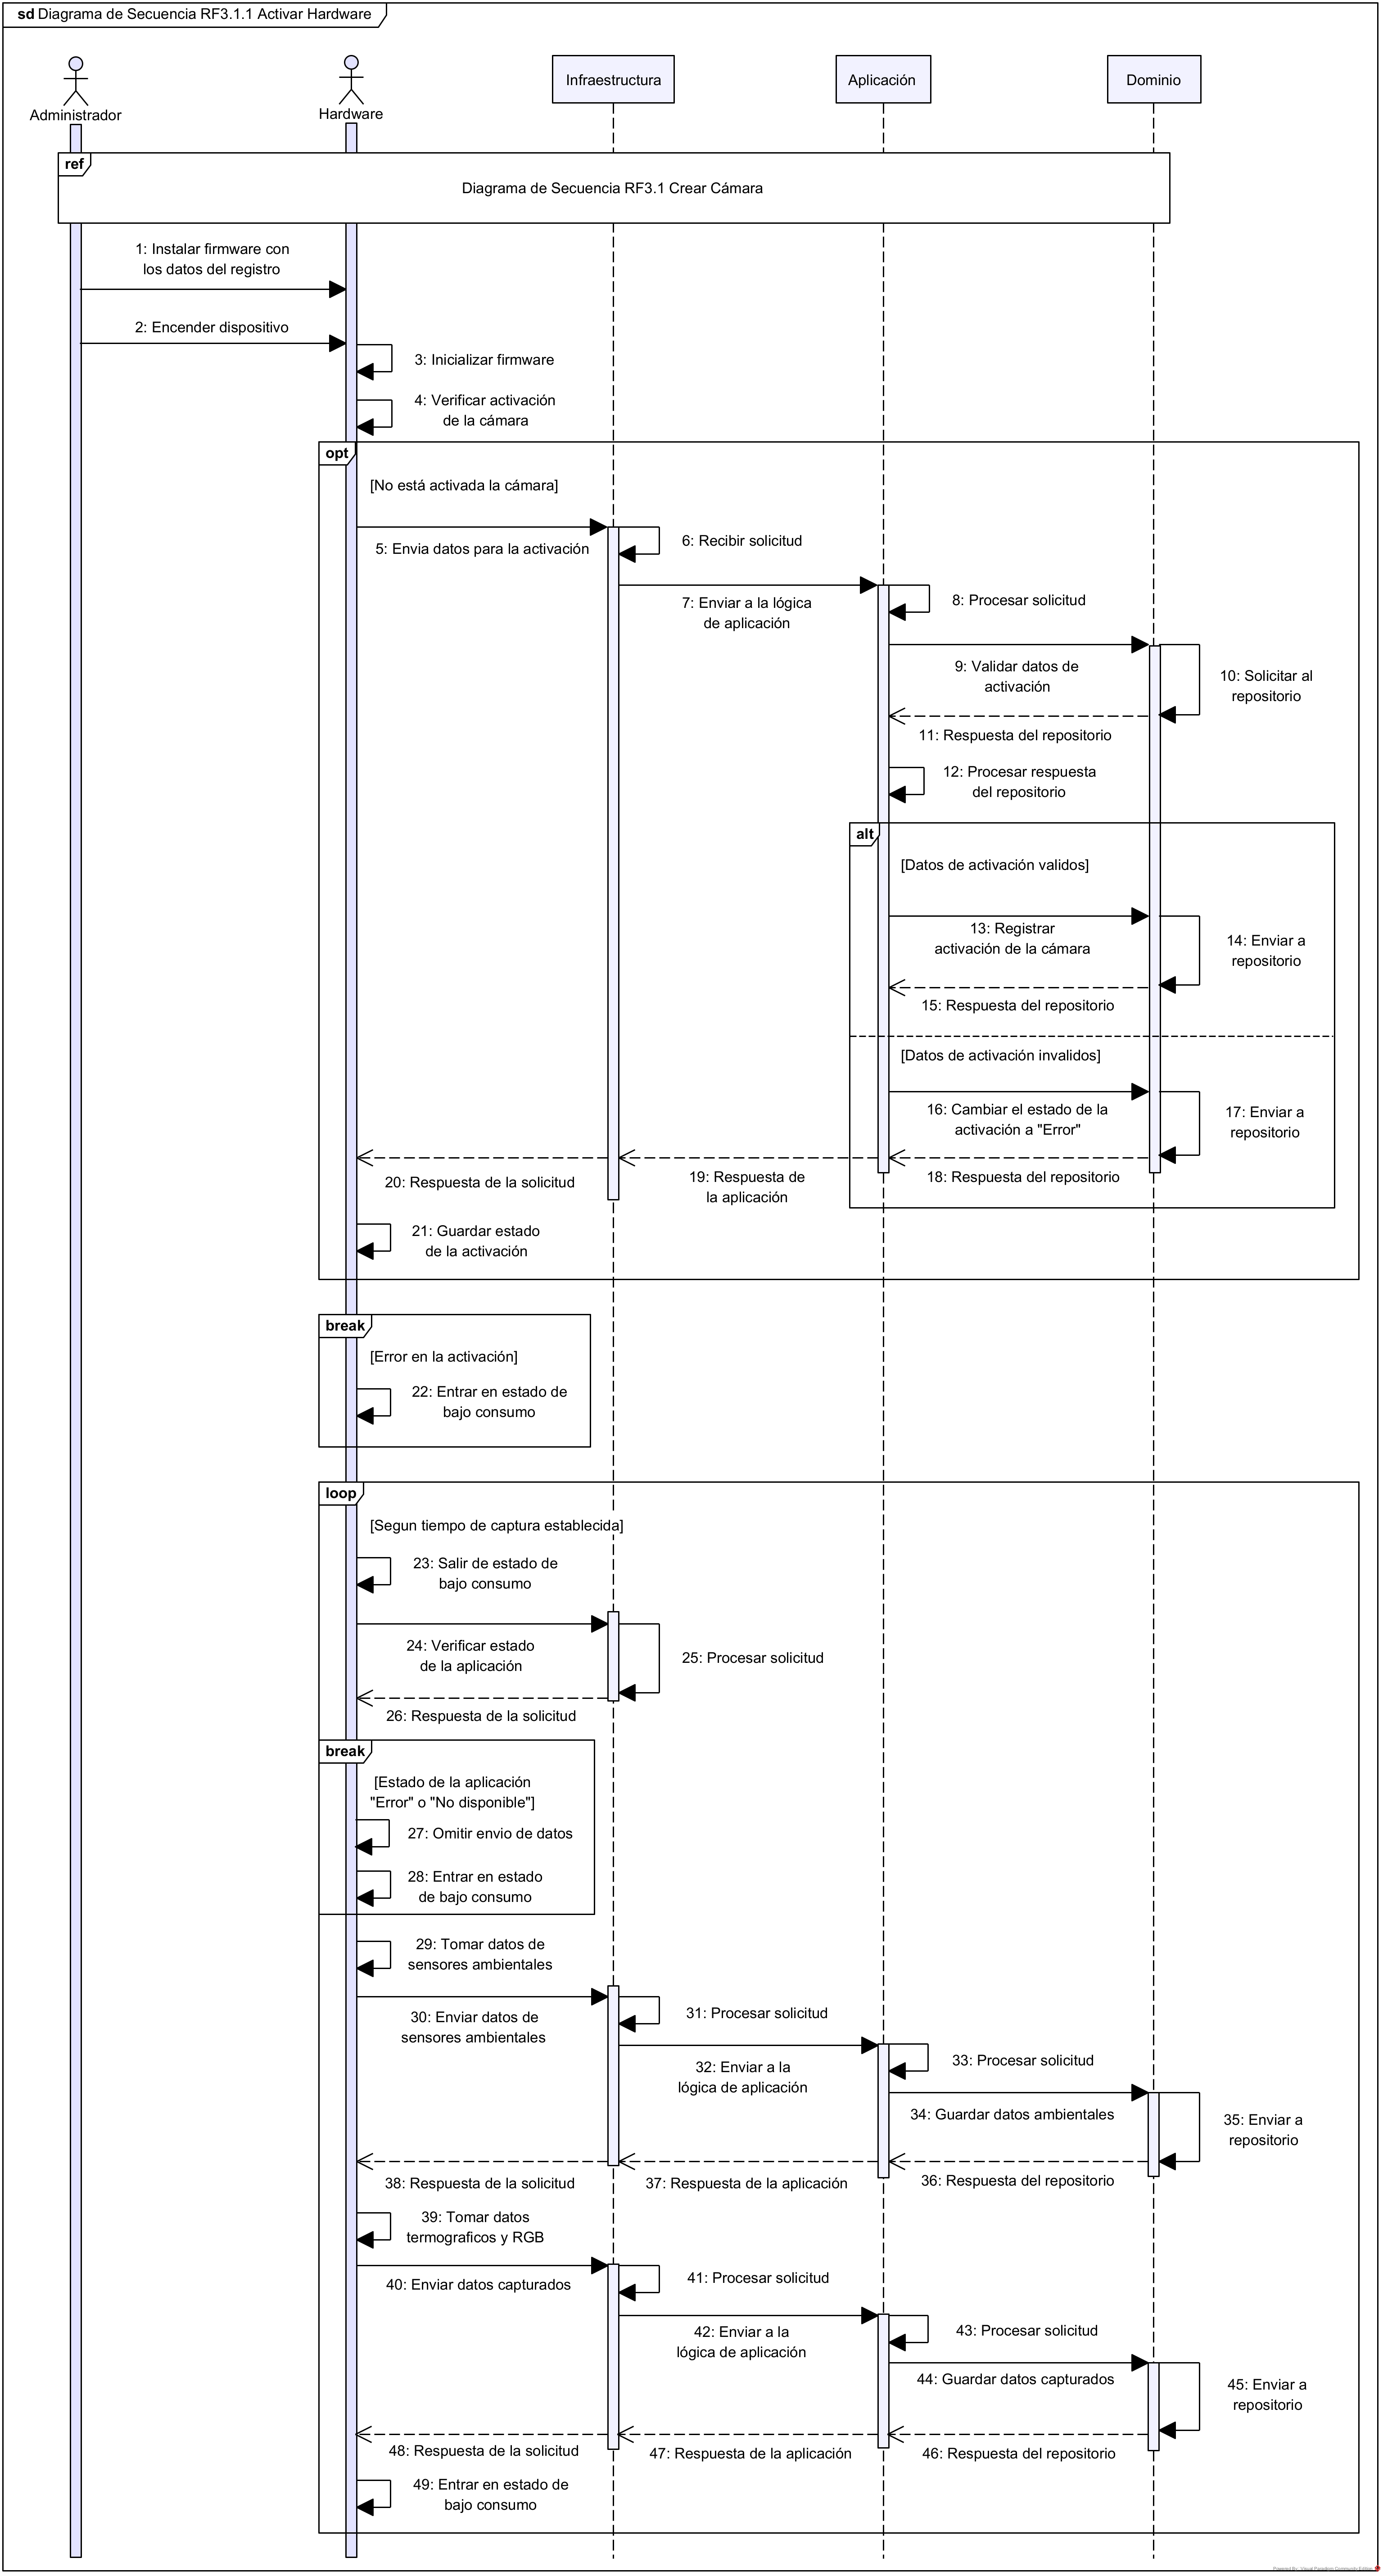
\includegraphics[width=0.6\textwidth]{UML/Secuencia/Diagrama de Secuencia RF3.1.1 Activar Hardware.png}
\end{figure}


\begin{figure}[H]
	\centering
		\caption{Diagrama de Secuencia para Consultar Cámara (RF3.2).}
	\includegraphics[width=0.8\textwidth]{UML/Secuencia/Diagrama de Secuencia RF3.2 Consultar Cámara.png}
\end{figure}


\begin{figure}[H]
	\centering
	\caption{Diagrama de Secuencia para Editar Cámara (RF3.3).}
 \includegraphics[width=0.8\textwidth]{UML/Secuencia/Diagrama de Secuencia RF3.3 Editar Cámara.png}
\end{figure}


\begin{figure}[H]
	\centering
		\caption{Diagrama de Secuencia para Eliminar Cámara (RF3.4).}
	\includegraphics[width=0.8\textwidth]{UML/Secuencia/Diagrama de Secuencia RF3.4 Eliminar Cámara.png}
\end{figure}


\begin{figure}[H]
	\centering
	\caption{Diagrama de Secuencia para Consultar Perfil (RF4.1).}
 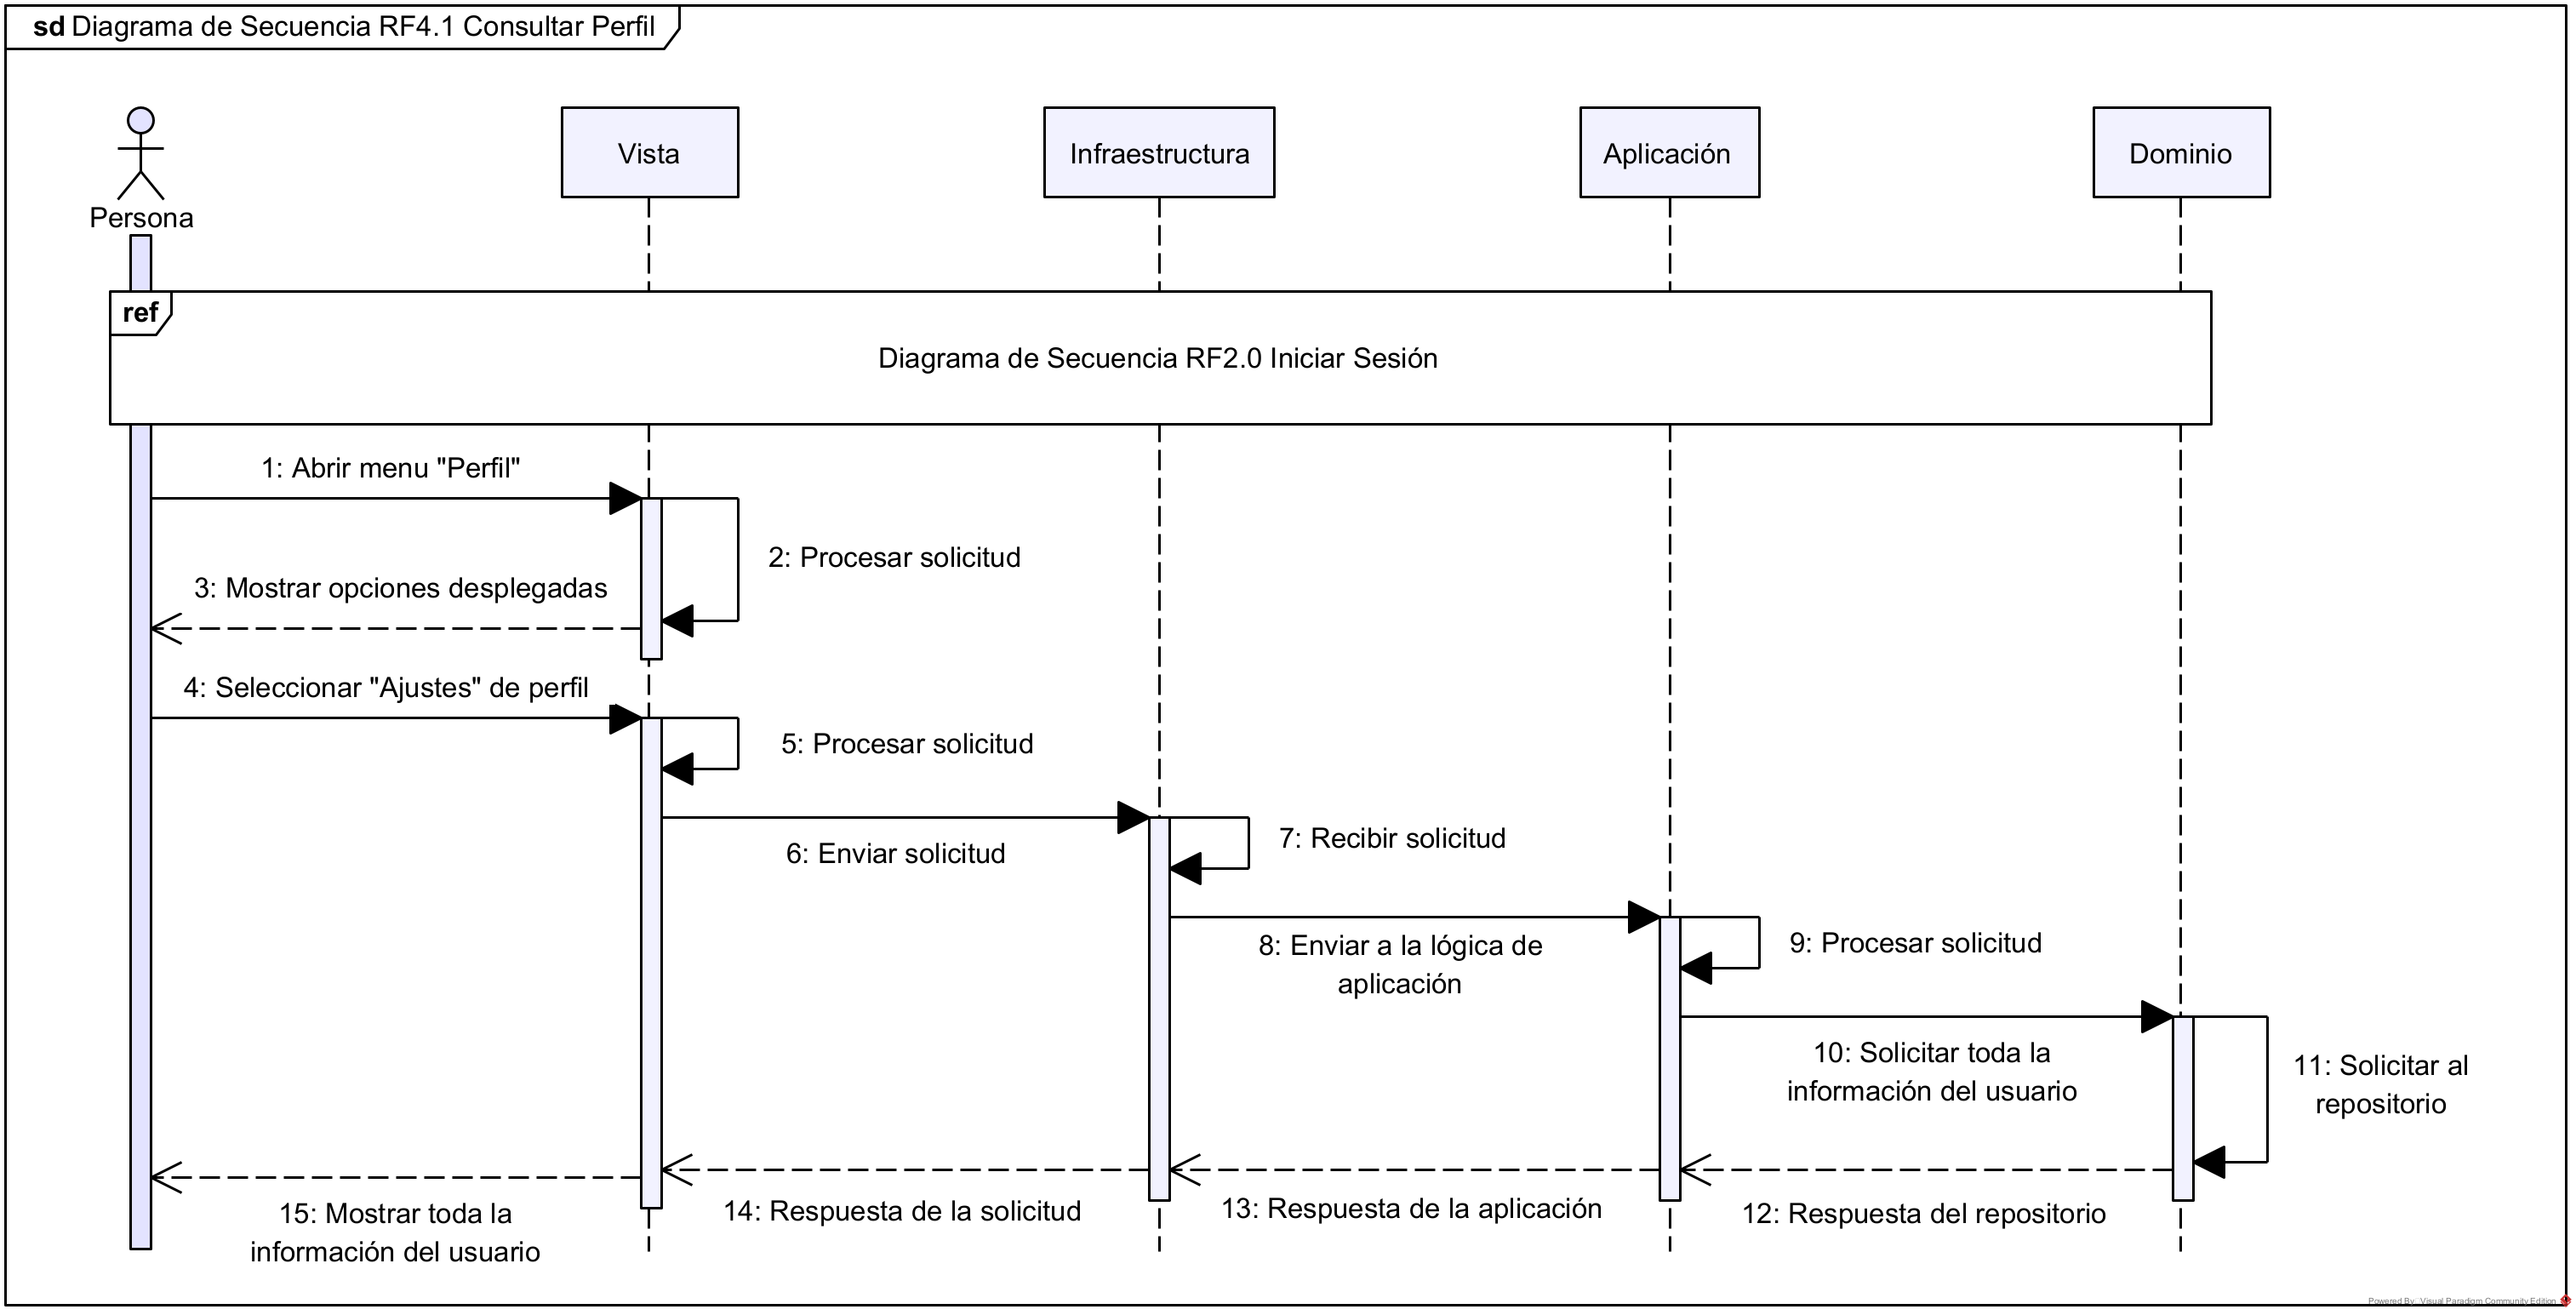
\includegraphics[width=0.8\textwidth]{UML/Secuencia/Diagrama de Secuencia RF4.1 Consultar Perfil.png}
\end{figure}


\begin{figure}[H]
	\centering
		\caption{Diagrama de Secuencia para Editar Perfil (RF4.2).}
	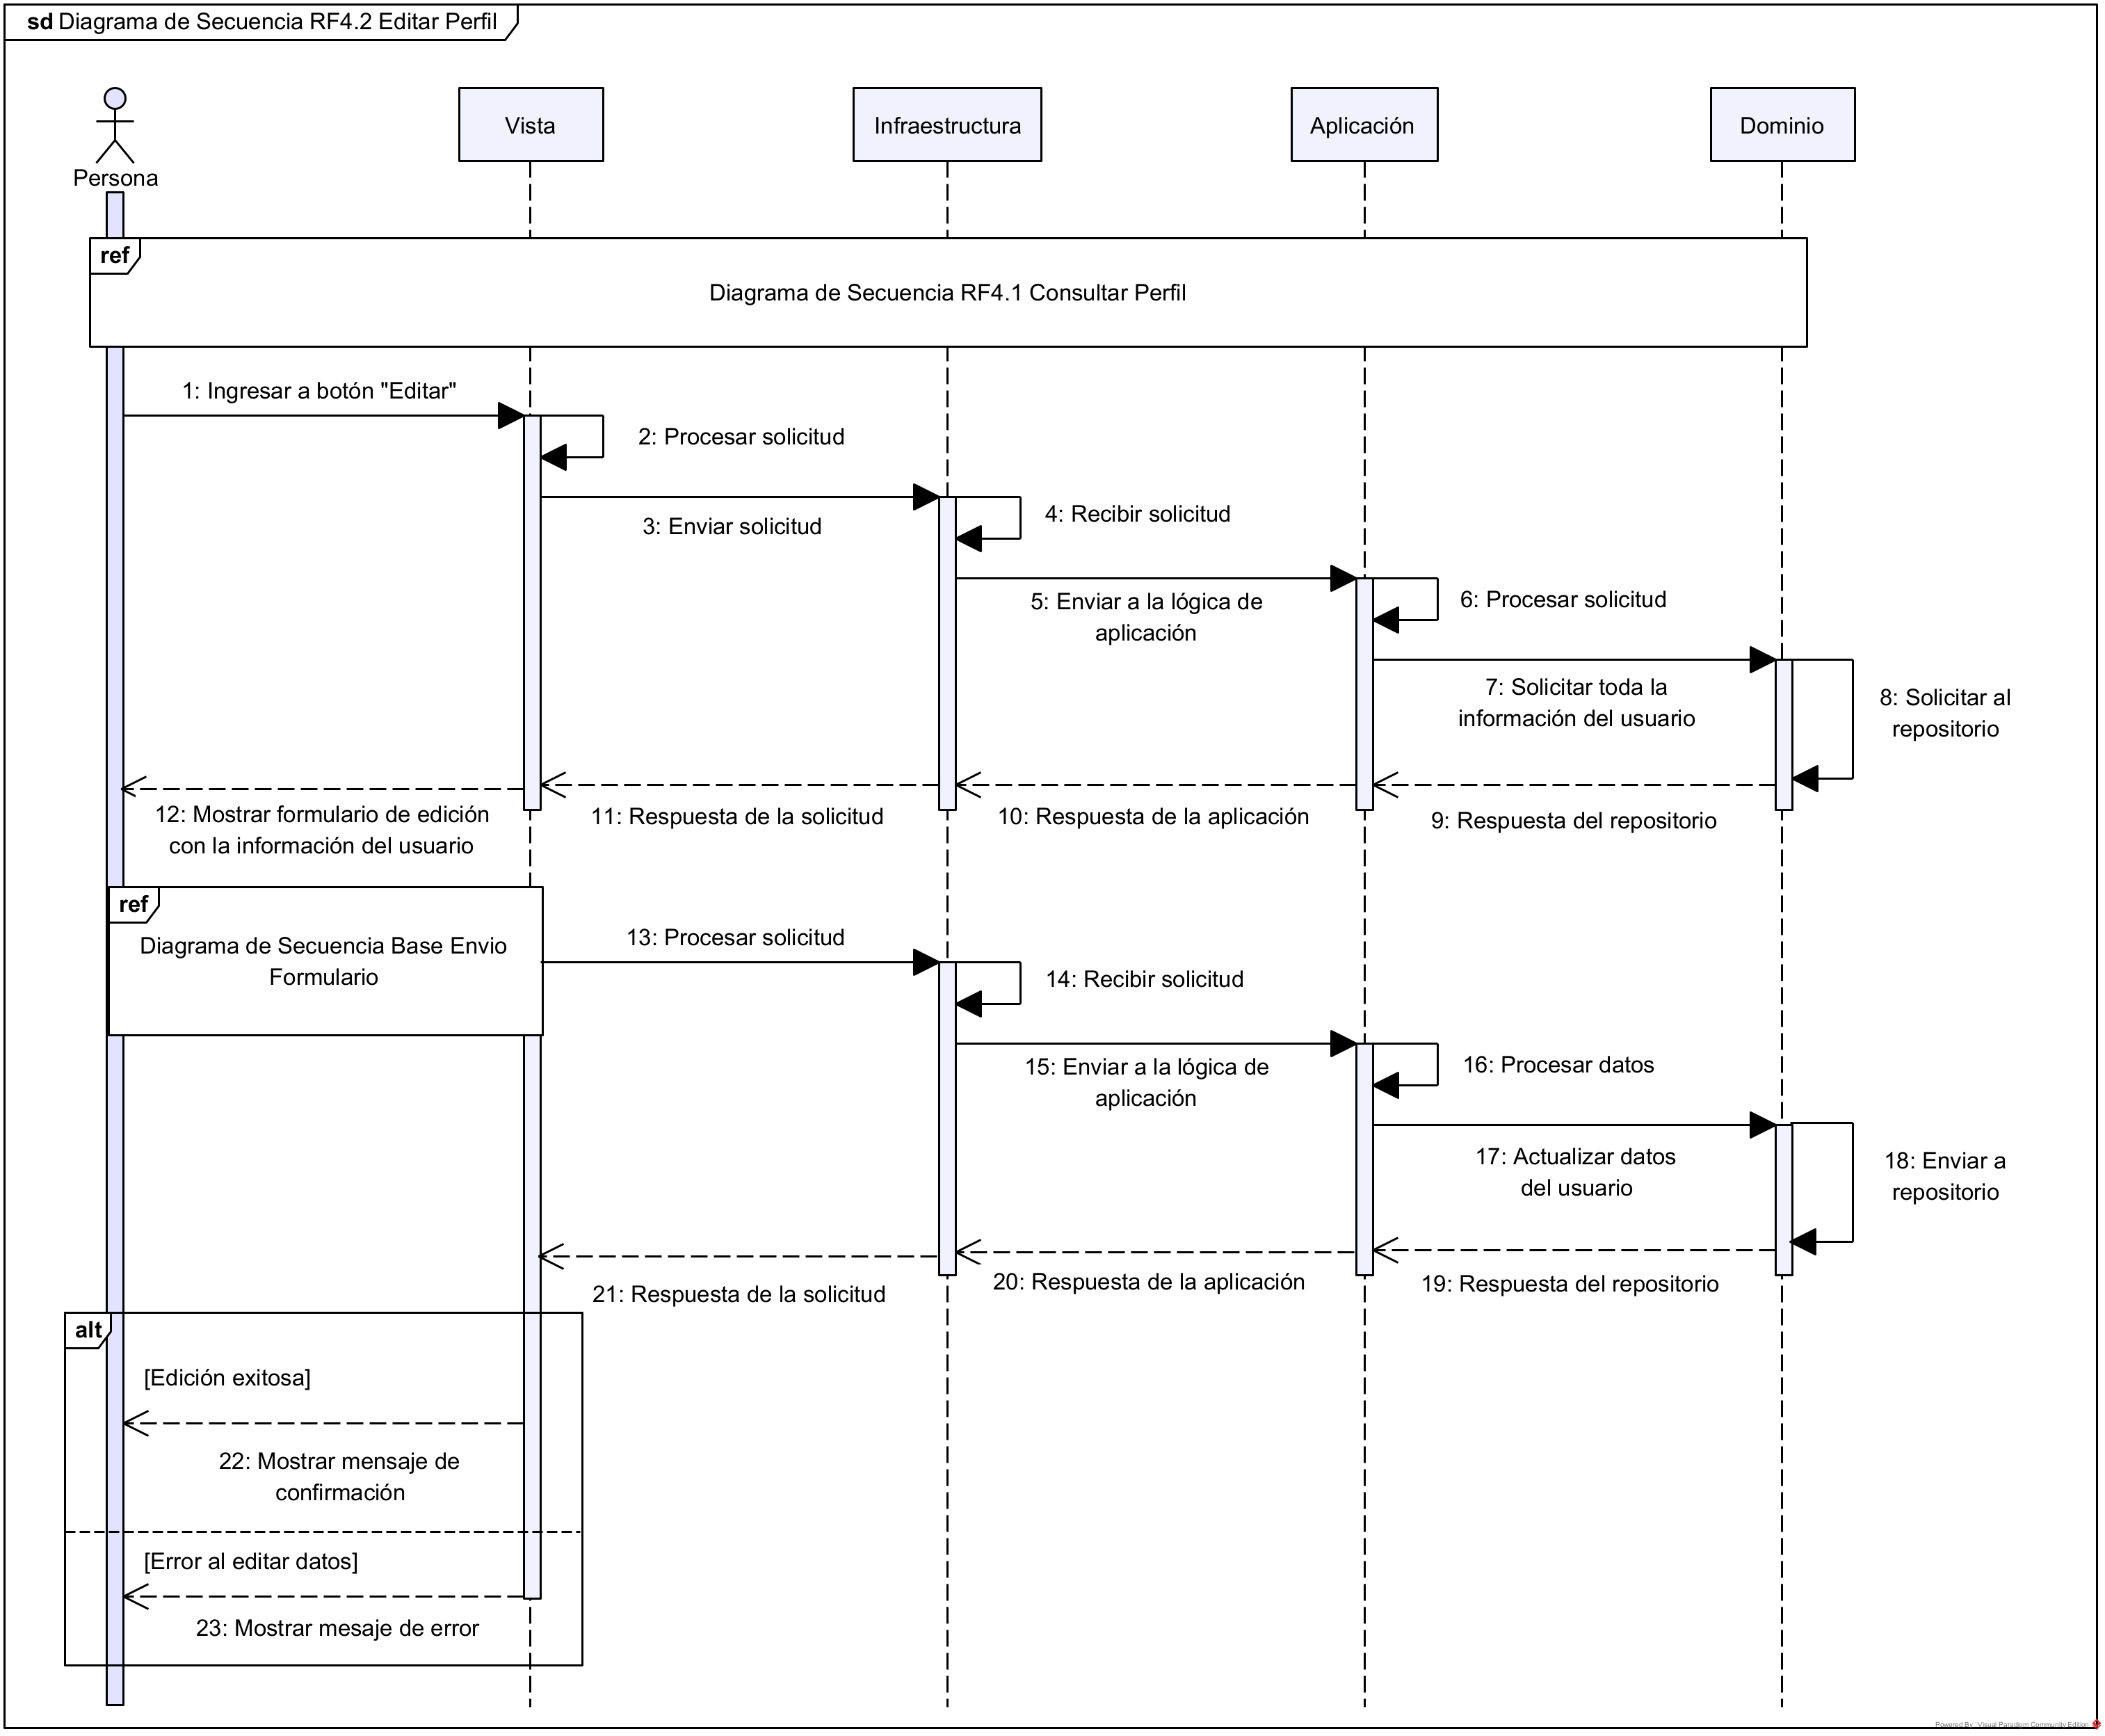
\includegraphics[width=0.8\textwidth]{UML/Secuencia/Diagrama de Secuencia RF4.2 Editar Perfil.png}
\end{figure}


\begin{figure}[H]
	\centering
	\caption{Diagrama de Secuencia para Eliminar Perfil (RF4.3).}
 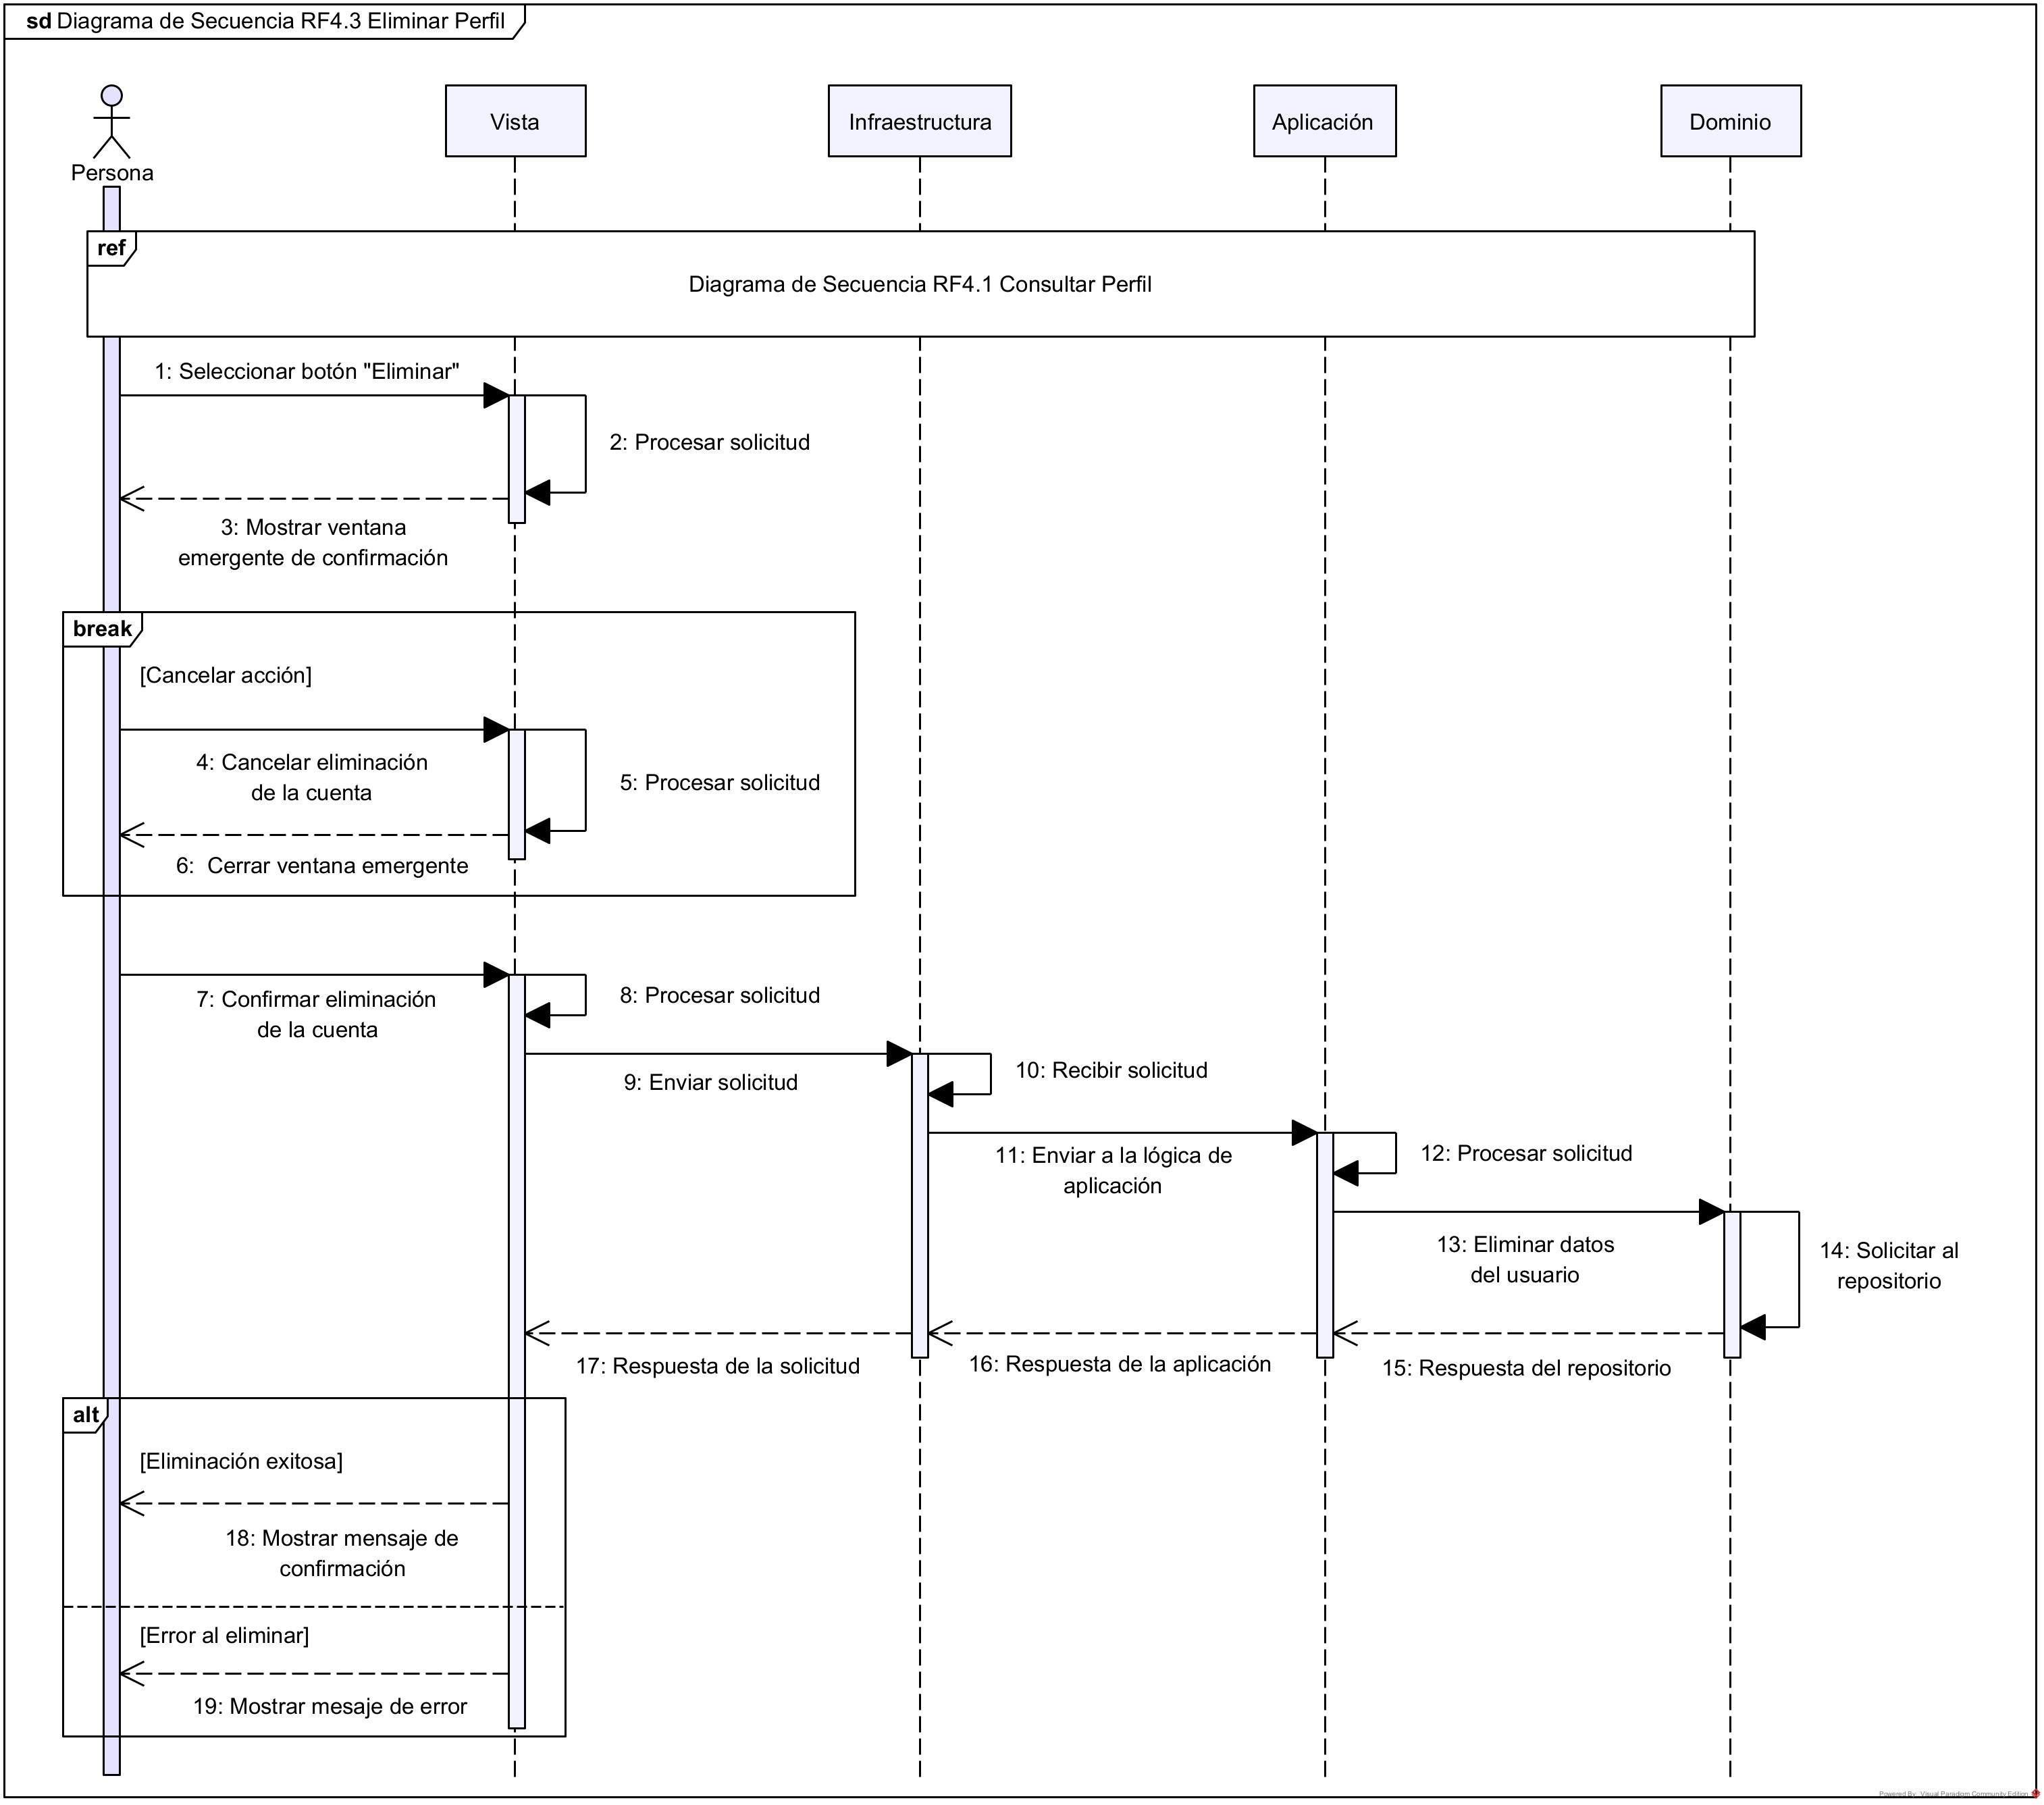
\includegraphics[width=0.8\textwidth]{UML/Secuencia/Diagrama de Secuencia RF4.3 Eliminar Perfil.png}
\end{figure}


\begin{figure}[H]
	\centering
		\caption{Diagrama de Secuencia para Cambiar Contraseña (RF4.4).}
	\includegraphics[width=0.8\textwidth]{UML/Secuencia/Diagrama de Secuencia RF4.4 Cambiar Contraseña.png}
\end{figure}


\begin{figure}[H]
	\centering
		\caption{Diagrama de Secuencia para Agregar Integrante de Cultivo (RF4.5).}
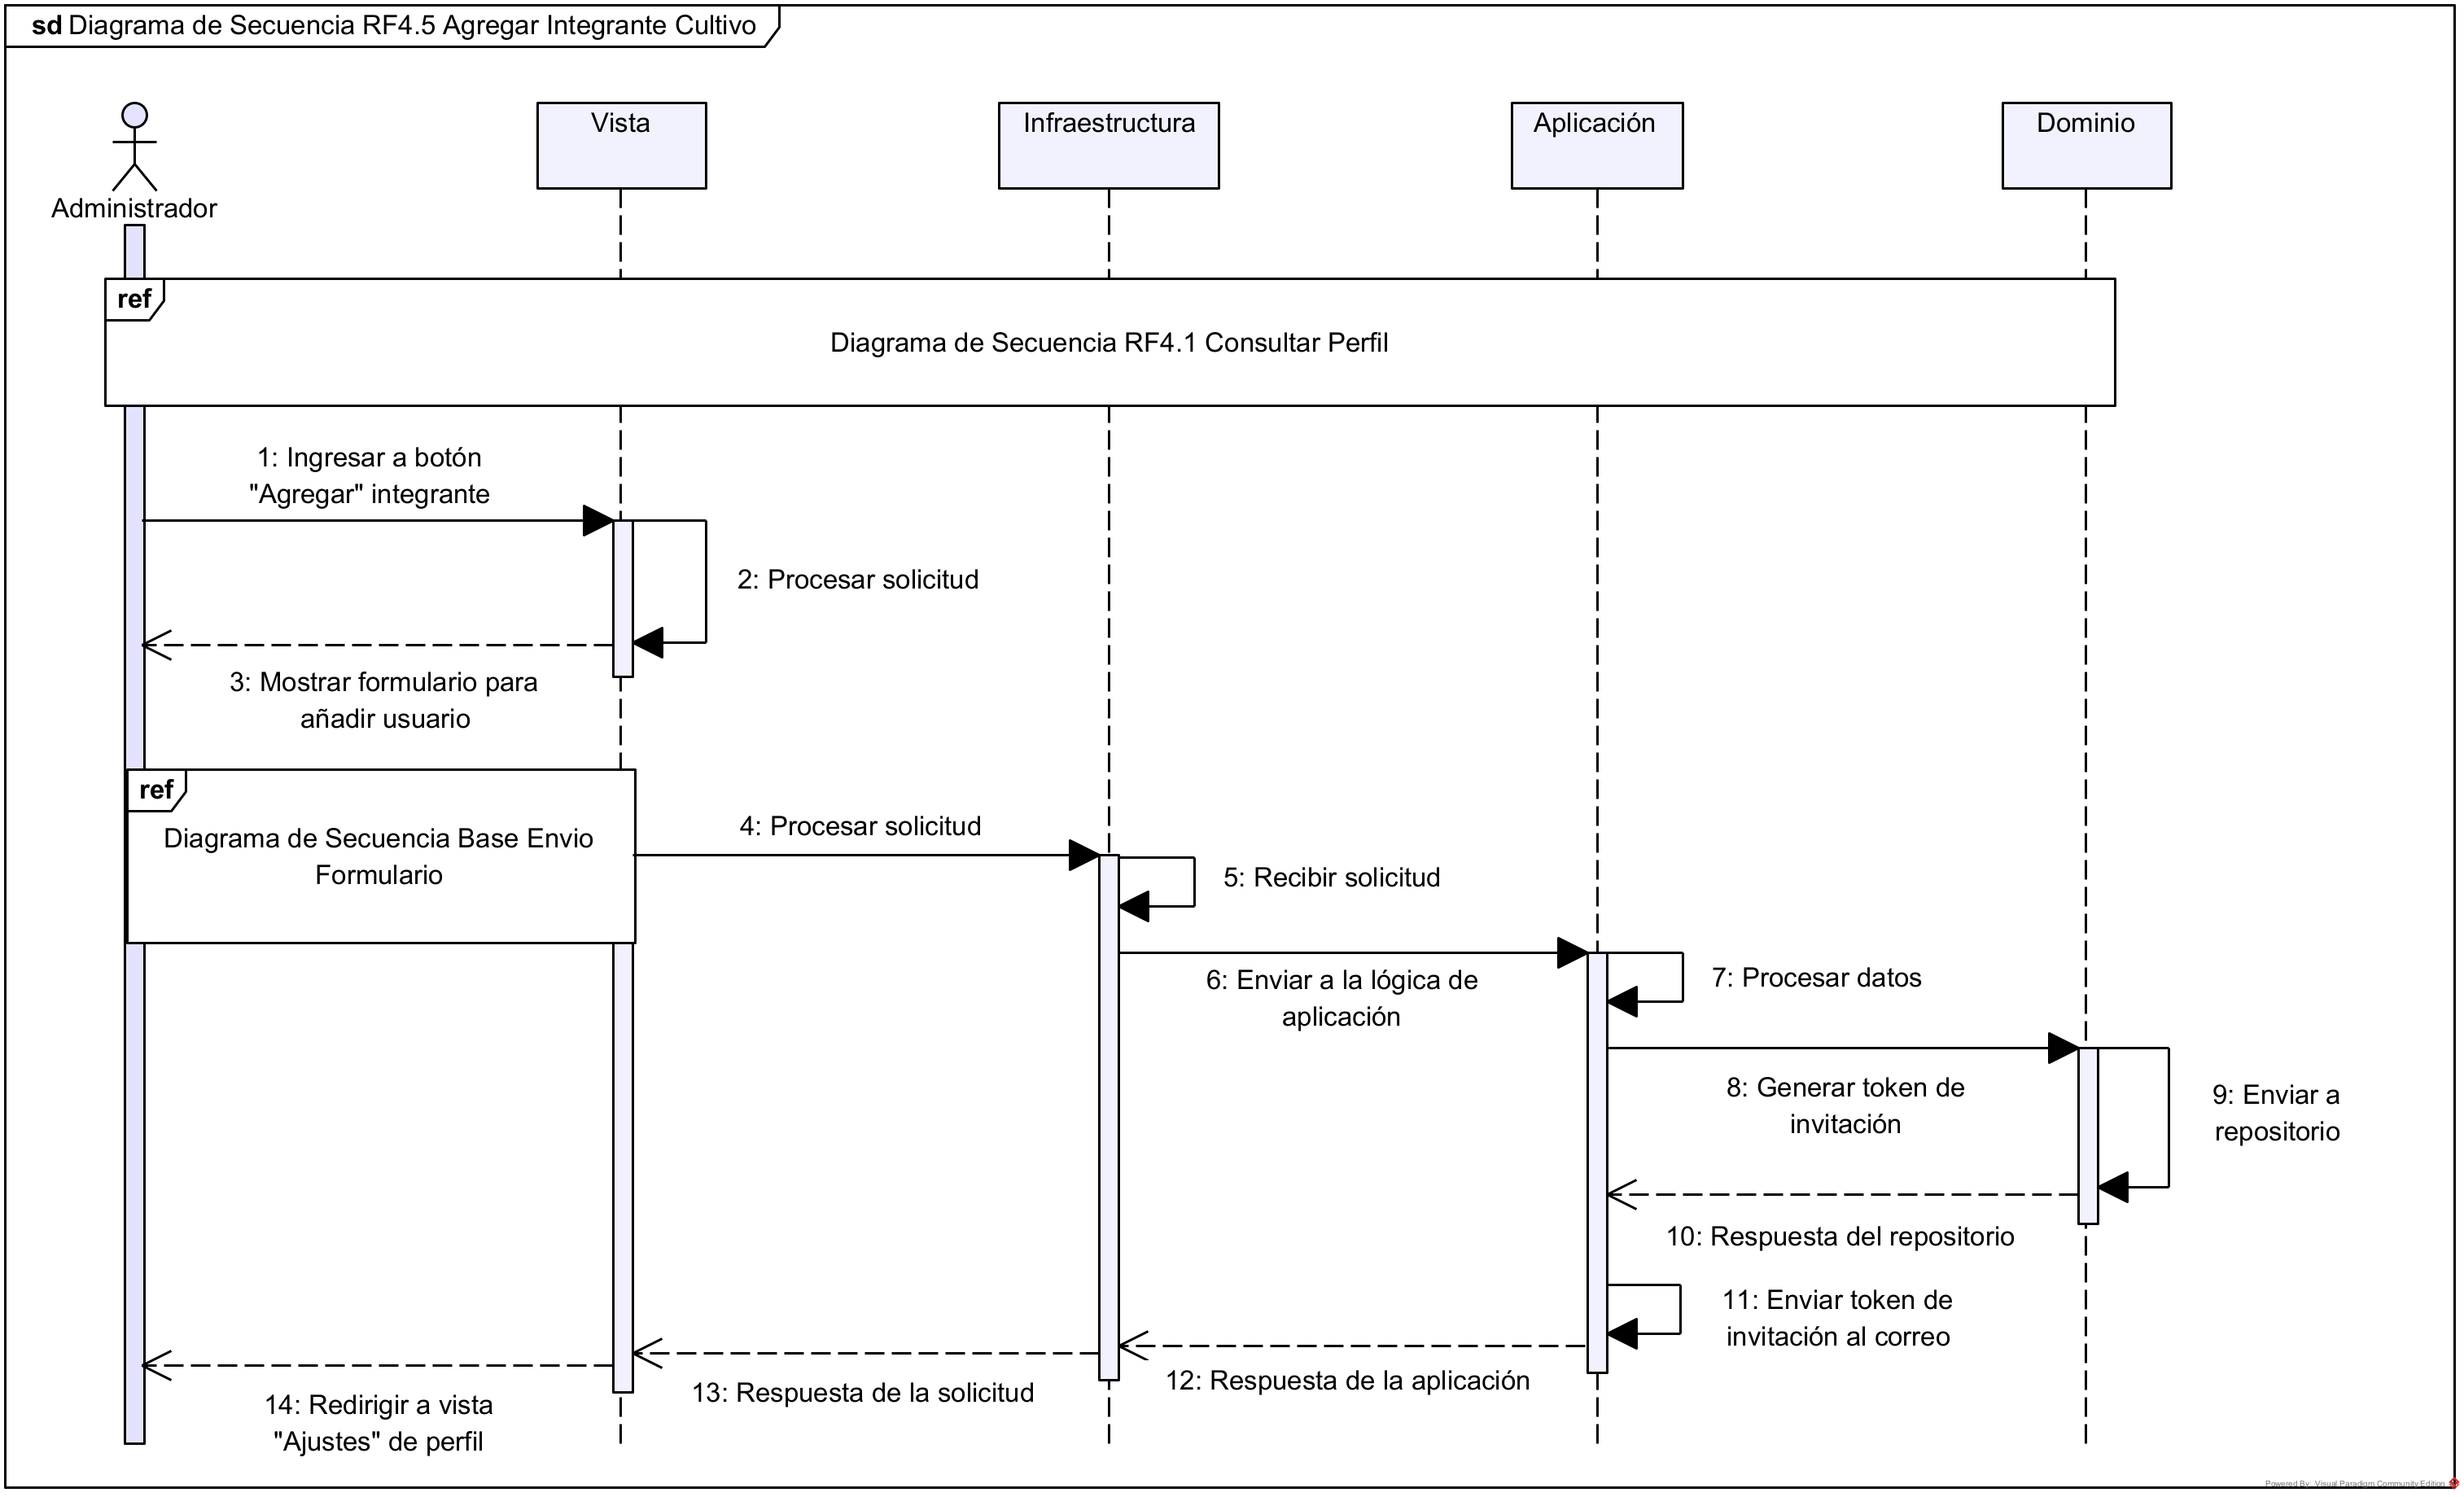
\includegraphics[width=0.8\textwidth]{UML/Secuencia/Diagrama de Secuencia RF4.5 Agregar Integrante Cultivo.png}
\end{figure}

\begin{figure}[H]
	\centering
	\caption{Diagrama de Secuencia para Eliminar Integrante de Cultivo (RF4.6).}
 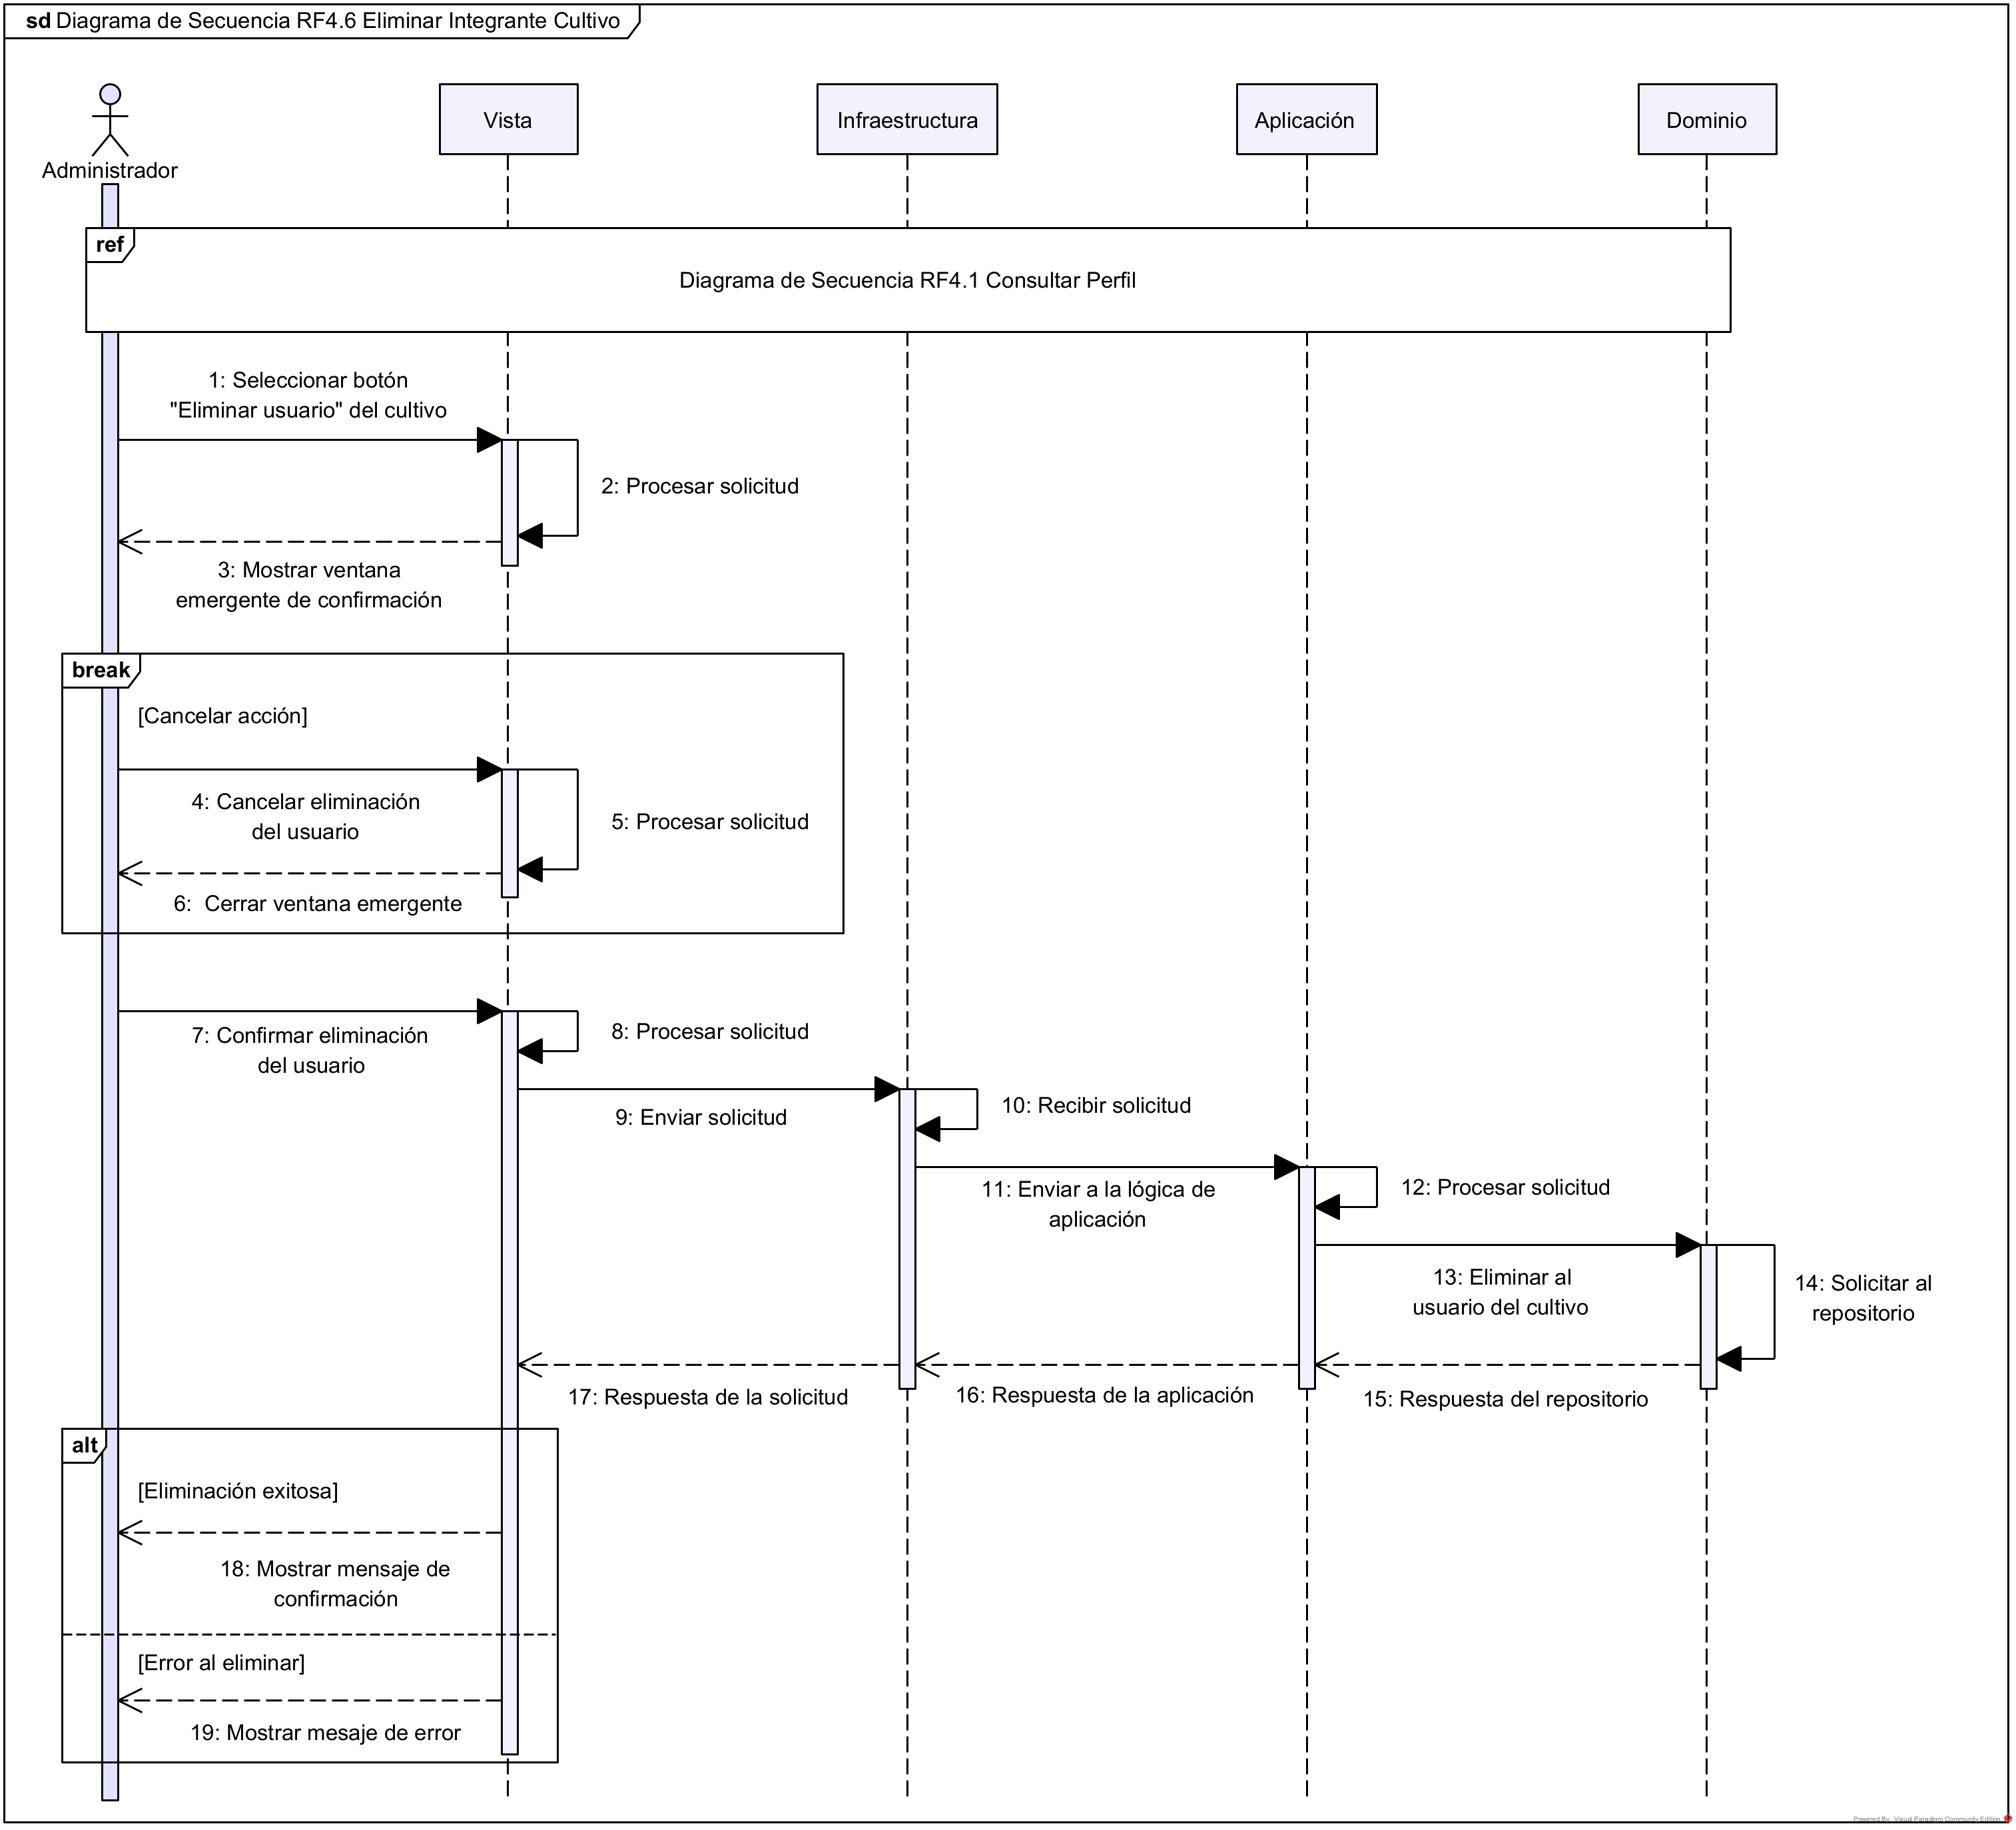
\includegraphics[width=0.8\textwidth]{UML/Secuencia/Diagrama de Secuencia RF4.6 Eliminar Integrante Cultivo.png}
\end{figure}


\begin{figure}[H]
	\centering
		\caption{Diagrama de Secuencia para el Módulo de Mediciones (RF5.0).}
	\includegraphics[width=0.8\textwidth]{UML/Secuencia/Diagrama de Secuencia RF5.0 Módulo de mediciones.png}
\end{figure}


\begin{figure}[H]
	\centering
	\caption{Diagrama de Secuencia para Crear Planta (RF6.1).}
 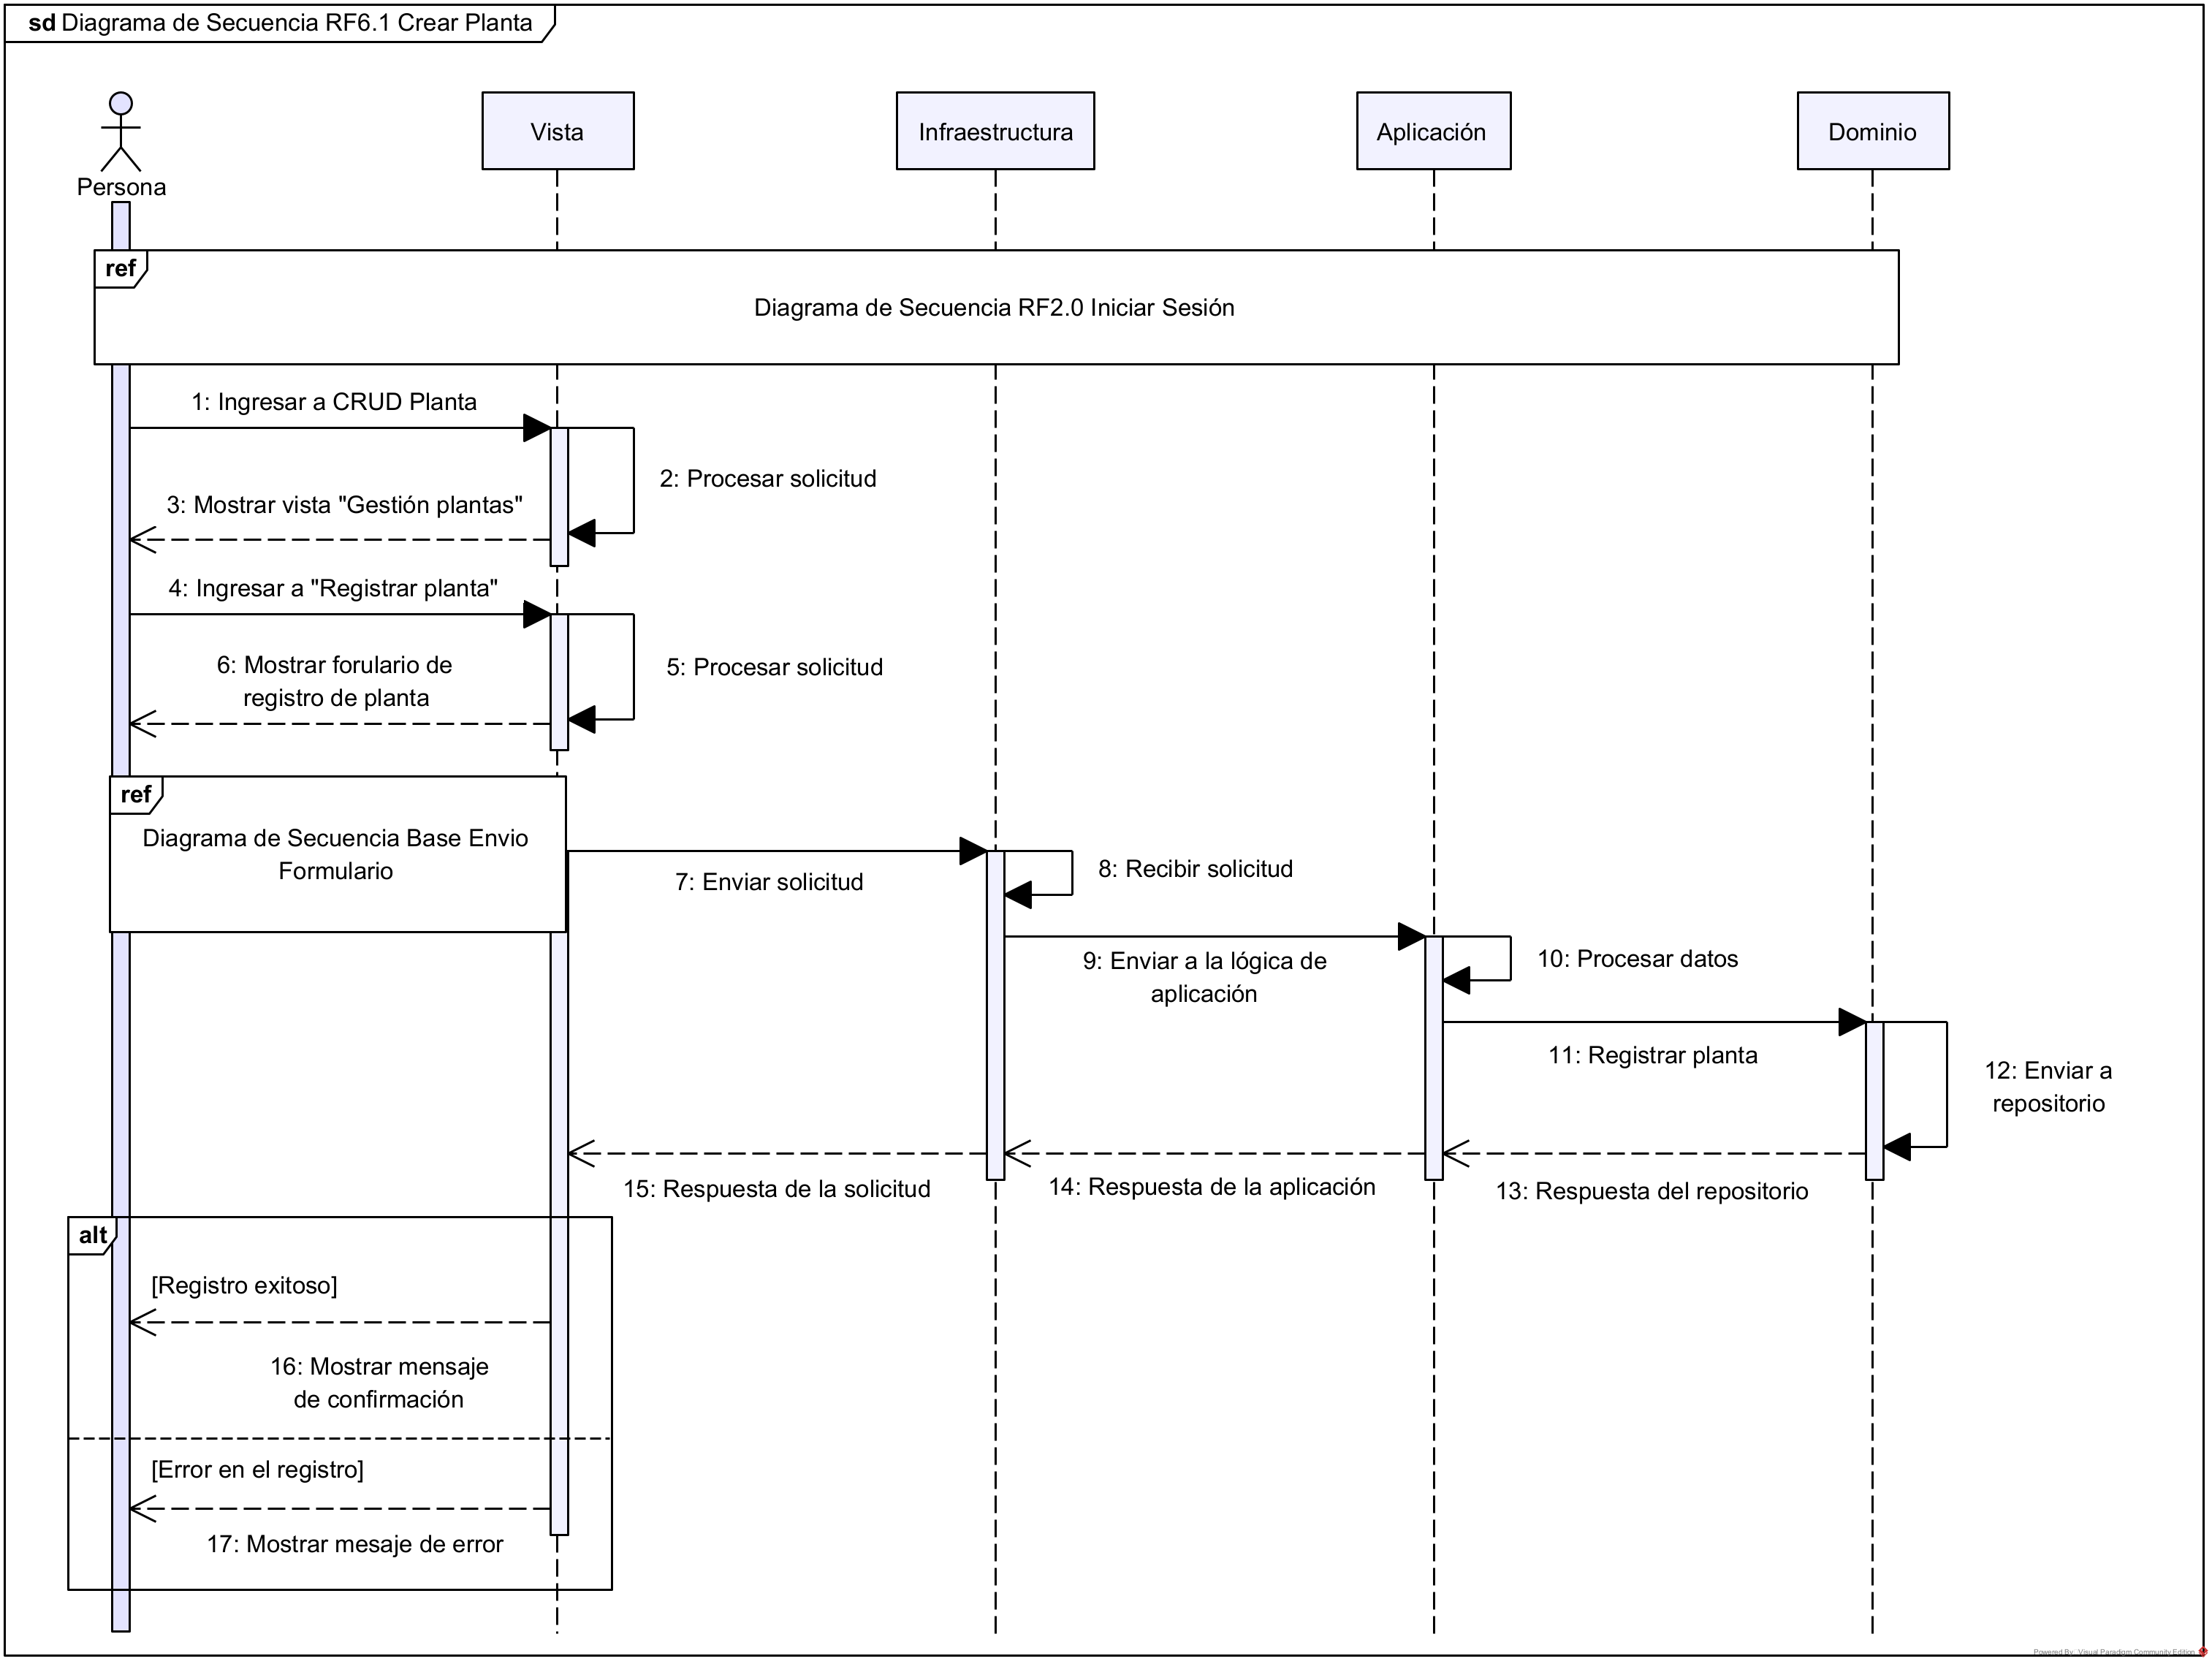
\includegraphics[width=0.8\textwidth]{UML/Secuencia/Diagrama de Secuencia RF6.1 Crear Planta.png}
\end{figure}


\begin{figure}[H]
	\centering
		\caption{Diagrama de Secuencia para Consultar Planta (RF6.2).}
	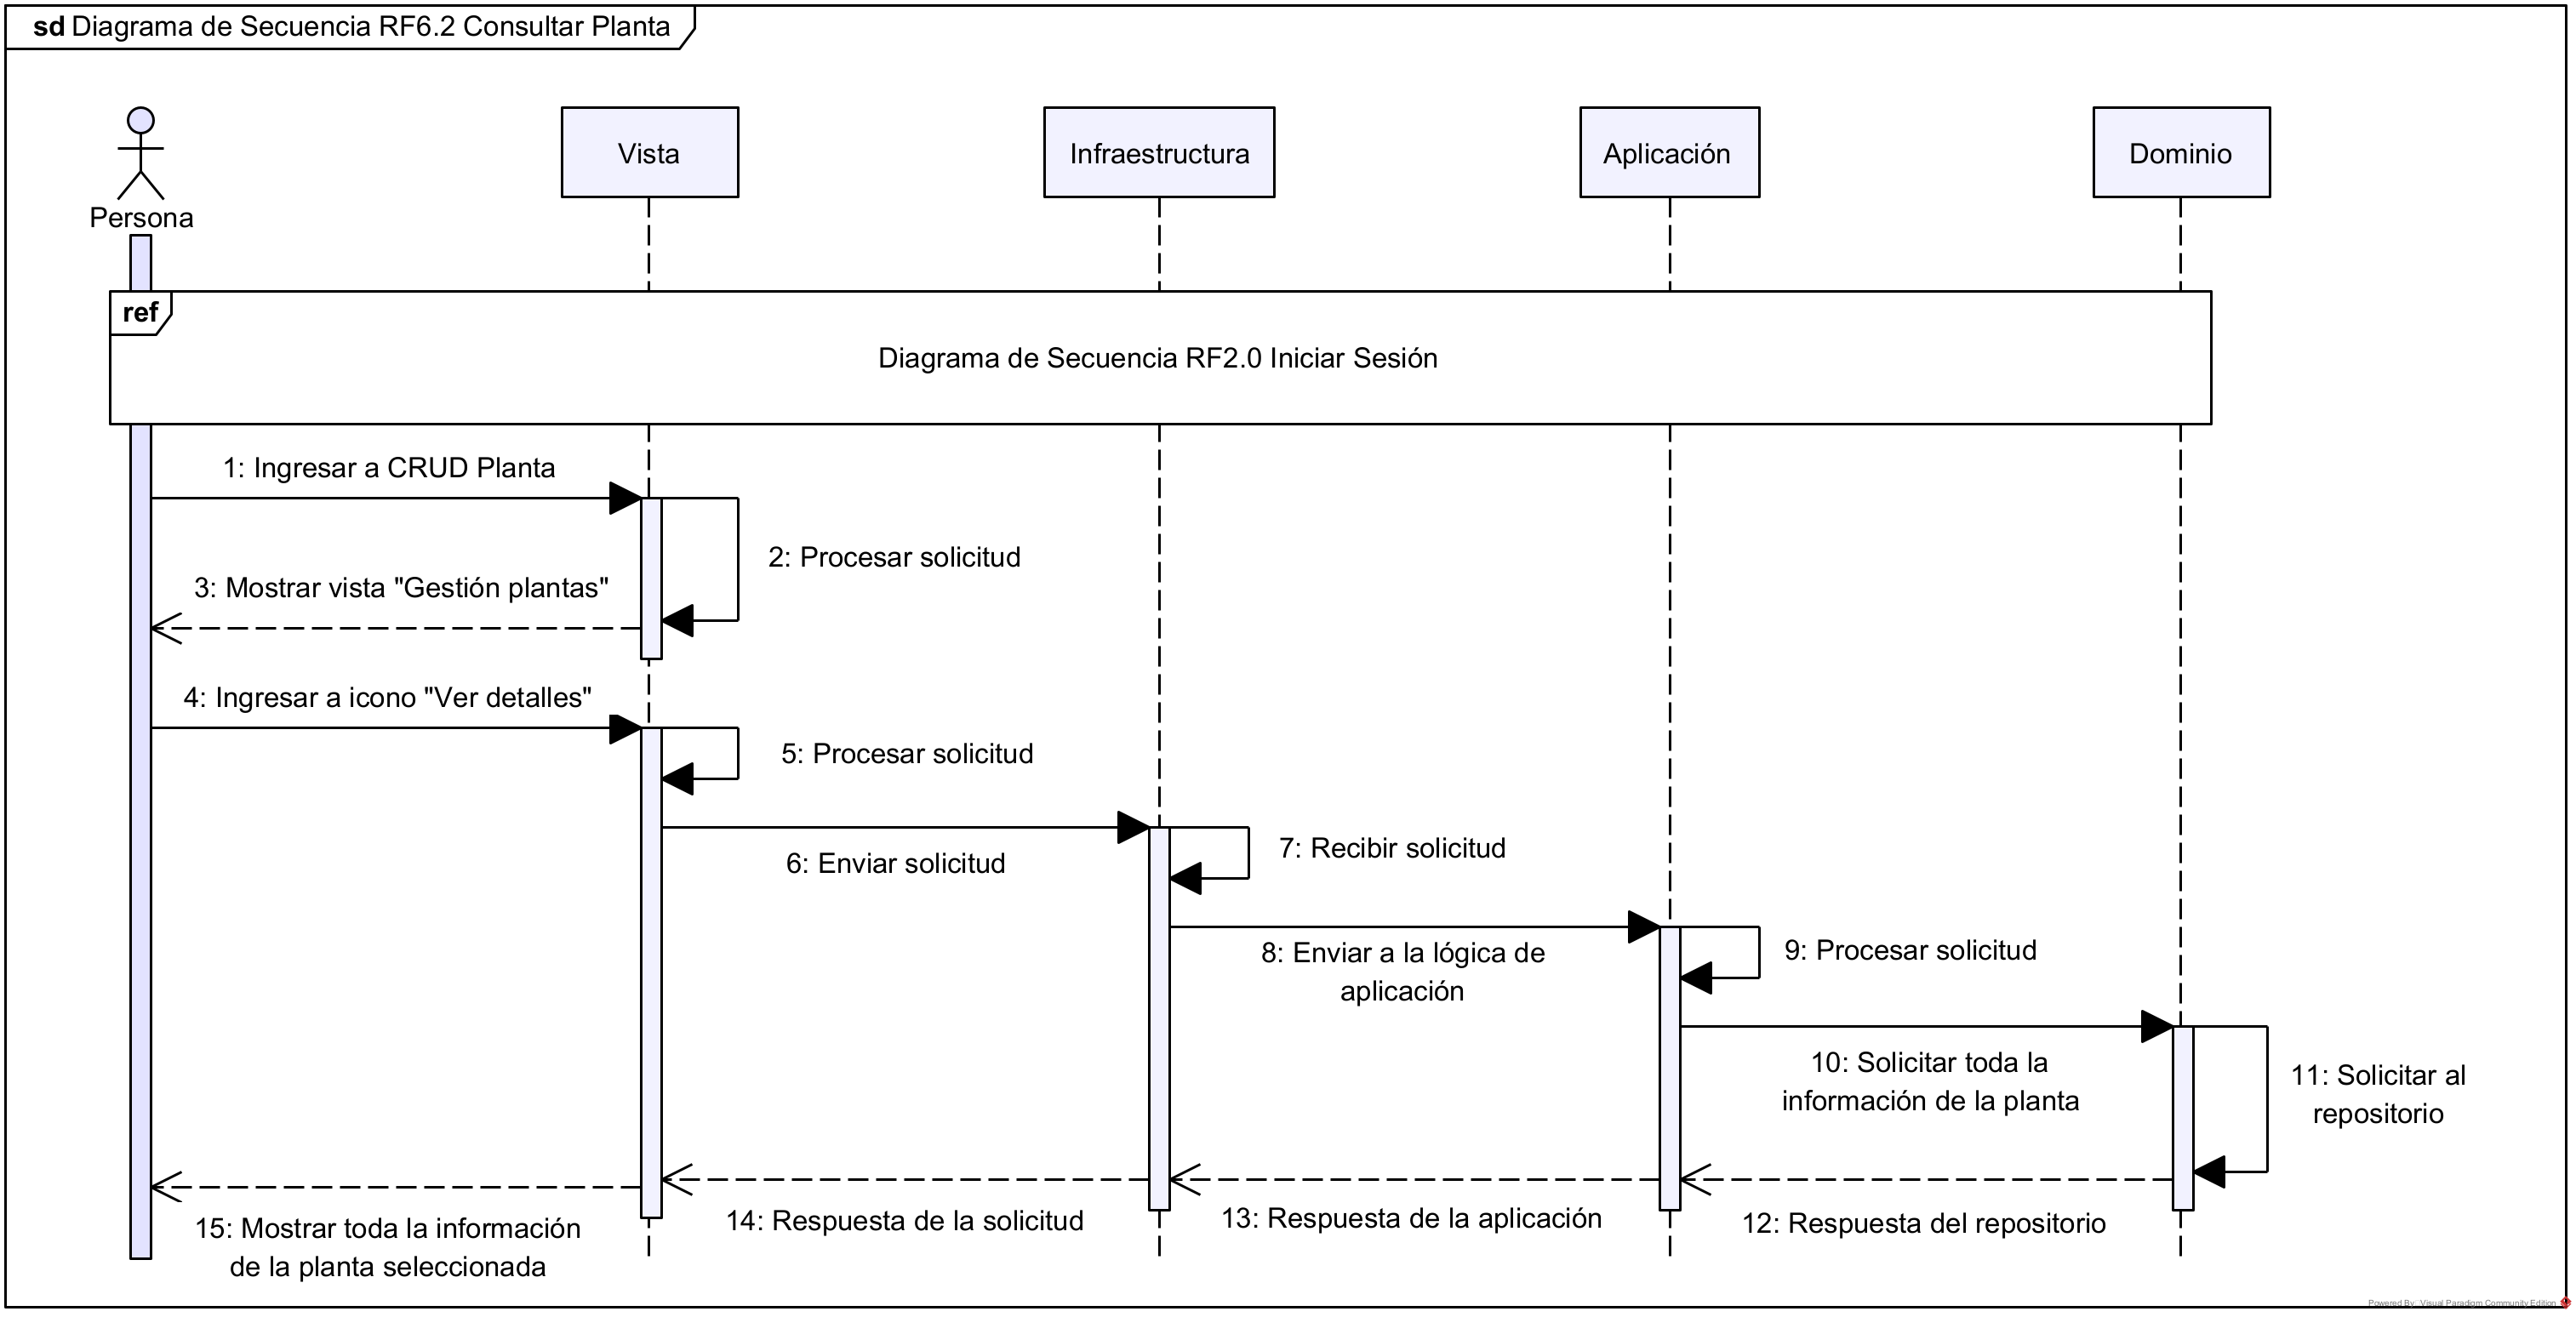
\includegraphics[width=0.8\textwidth]{UML/Secuencia/Diagrama de Secuencia RF6.2 Consultar Planta.png}
\end{figure}


\begin{figure}[H]
	\centering
	\caption{Diagrama de Secuencia para Editar Planta (RF6.3).}
 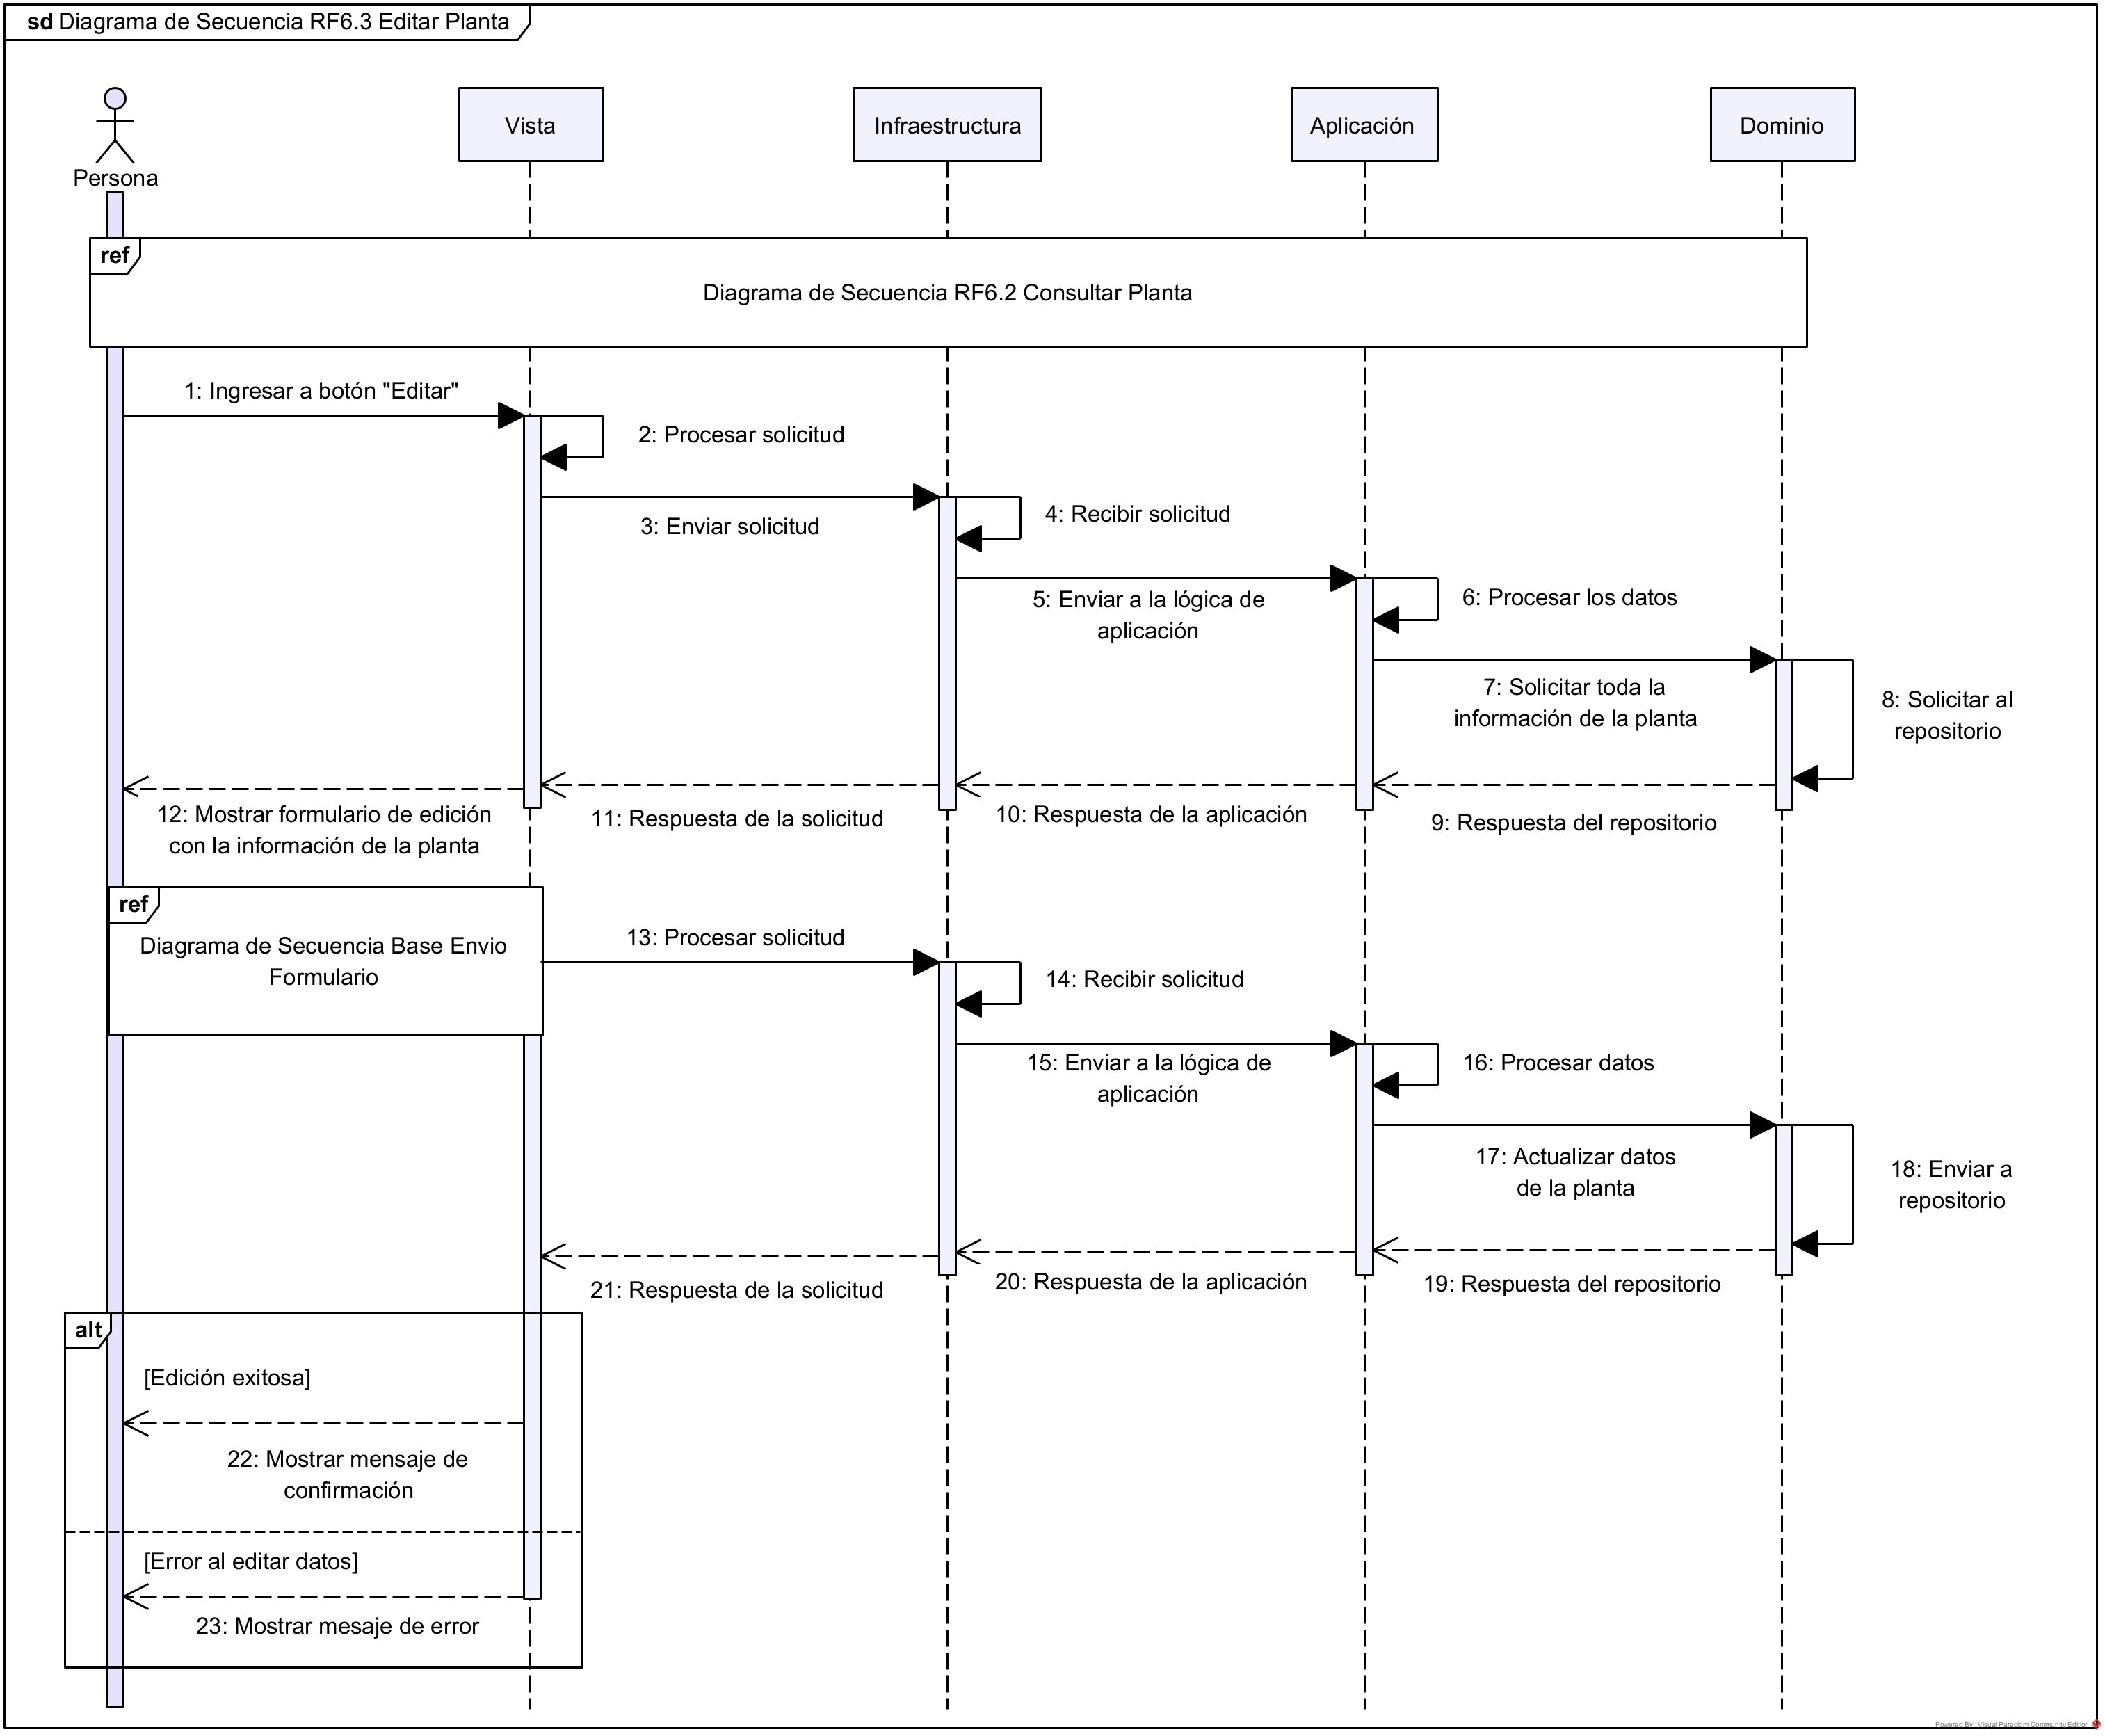
\includegraphics[width=0.8\textwidth]{UML/Secuencia/Diagrama de Secuencia RF6.3 Editar Planta.png}
\end{figure}


\begin{figure}[H]
	\centering
	\caption{Diagrama de Secuencia para Eliminar Planta (RF6.4).}
 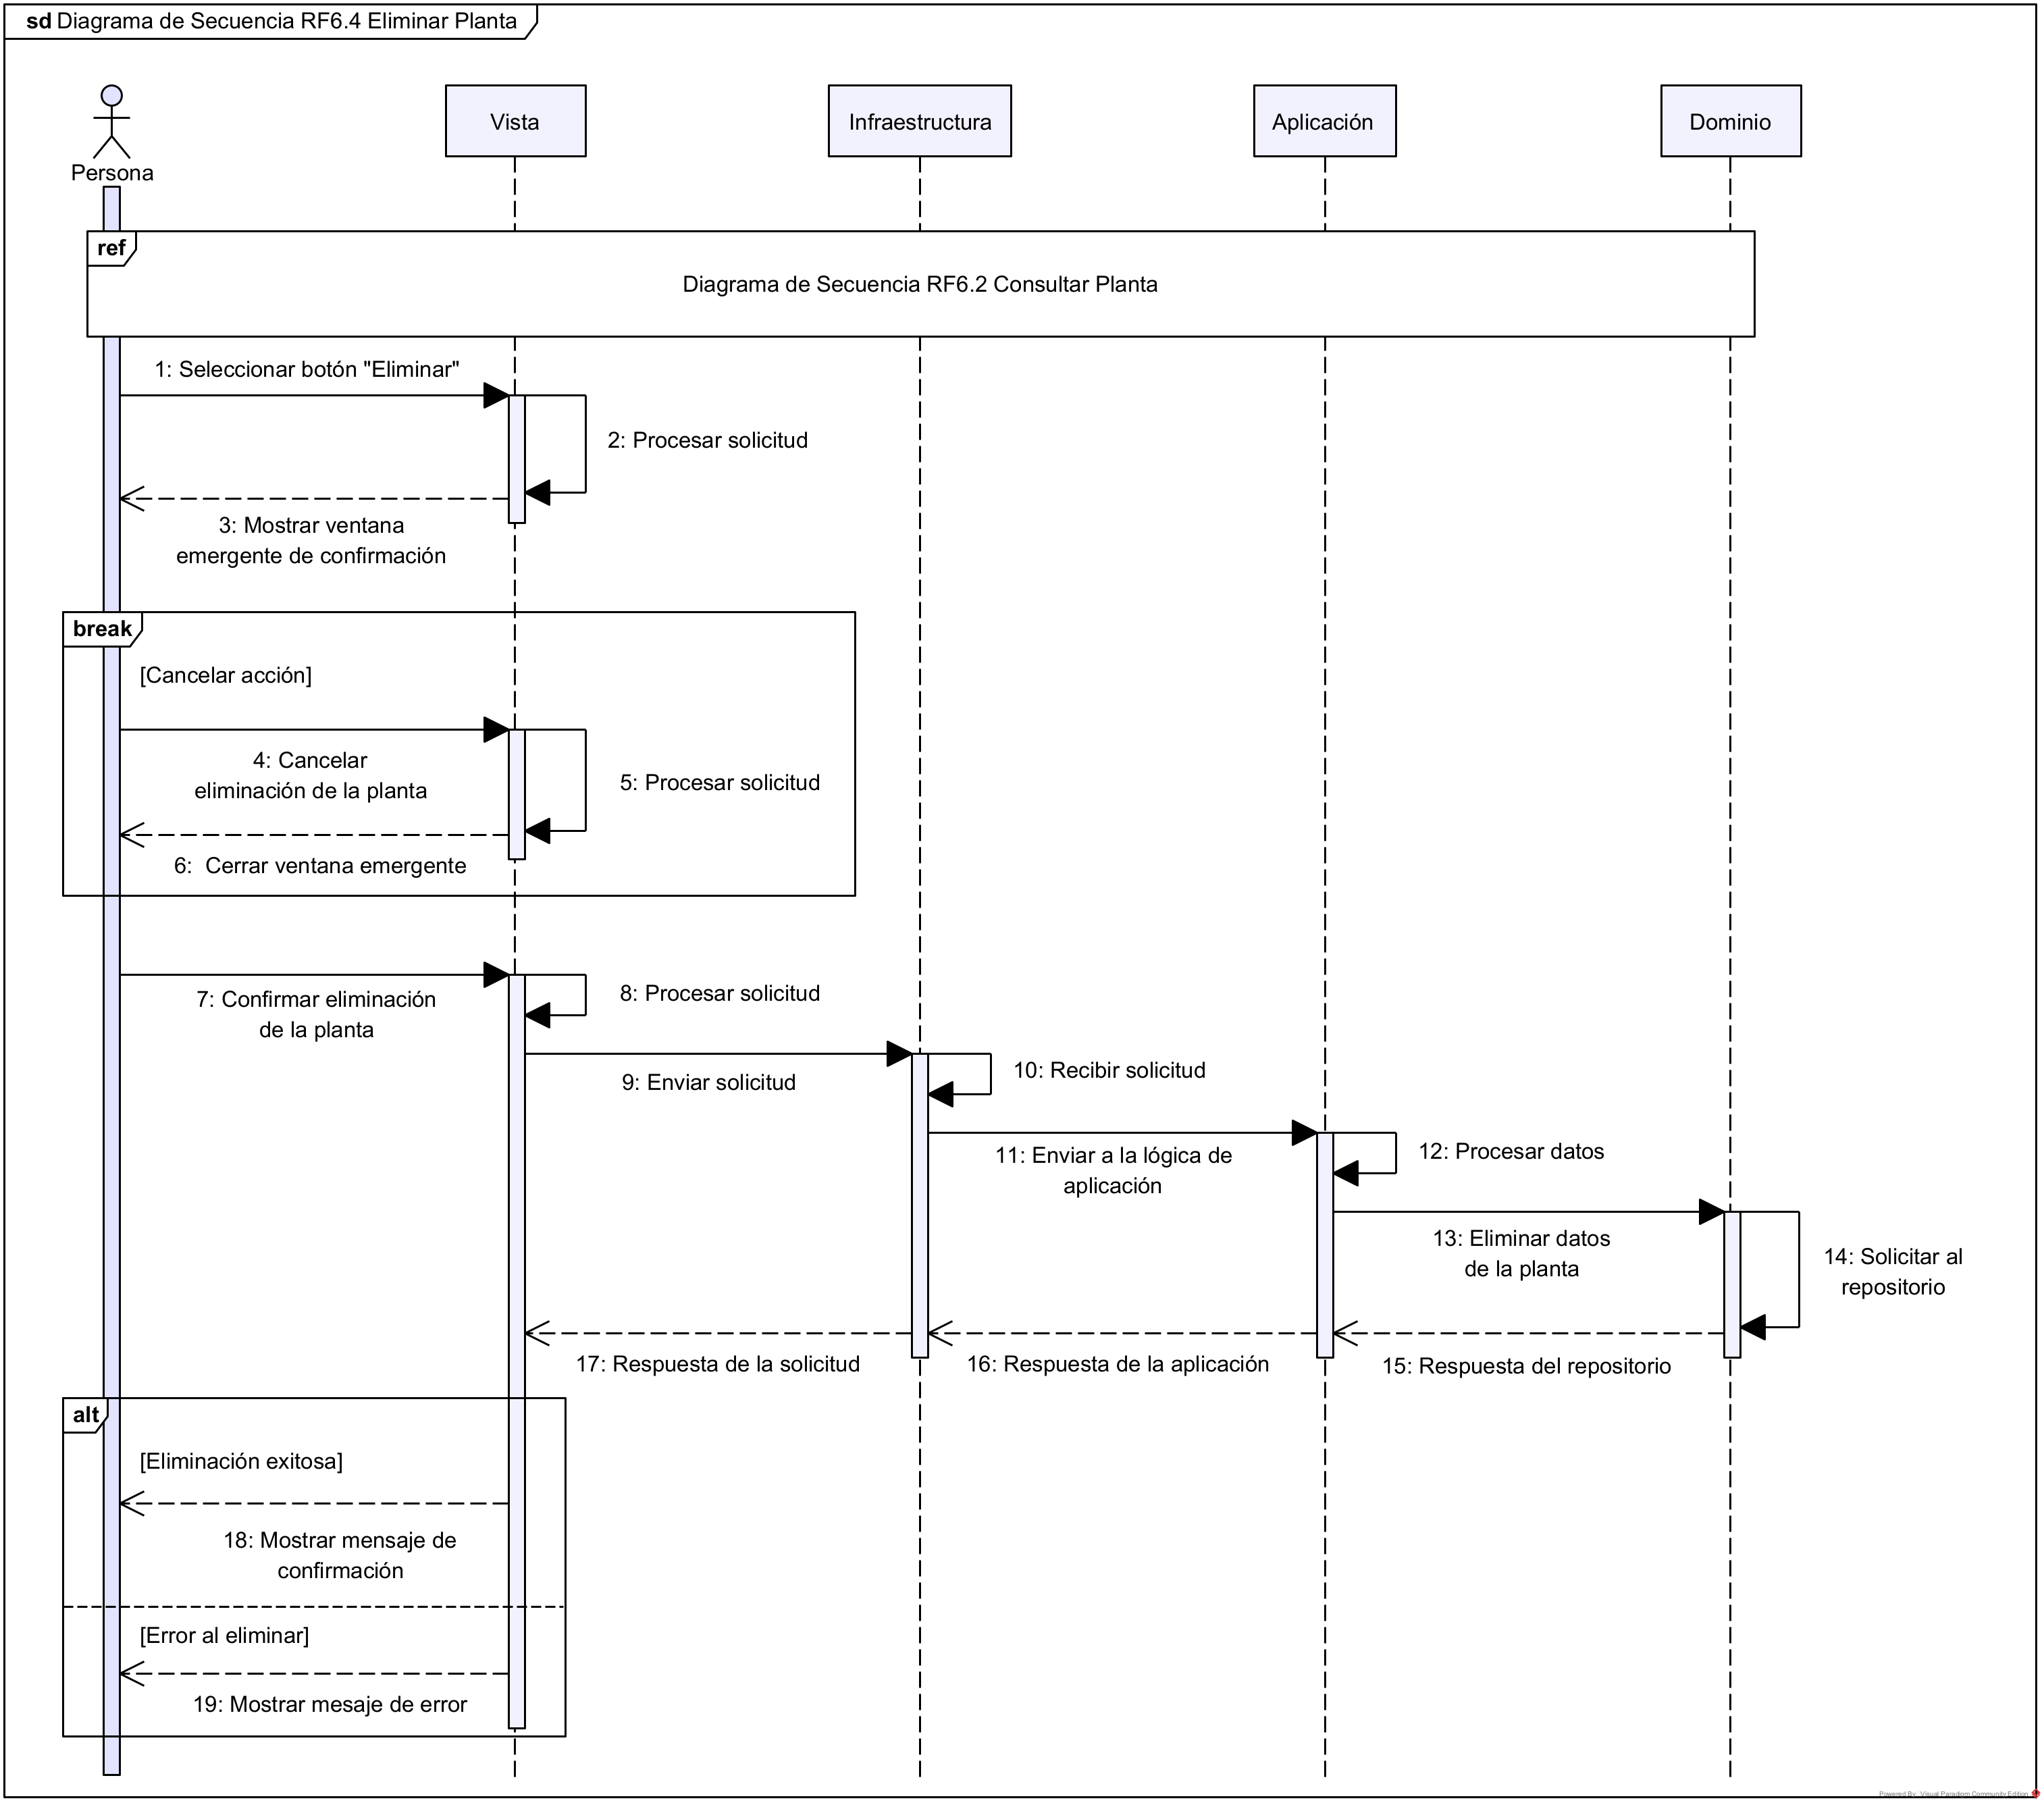
\includegraphics[width=0.8\textwidth]{UML/Secuencia/Diagrama de Secuencia RF6.4 Eliminar Planta.png}
\end{figure}


\begin{figure}[H]
	\centering
		\caption{Diagrama de Secuencia para Generar Reporte (RF7.0).}
	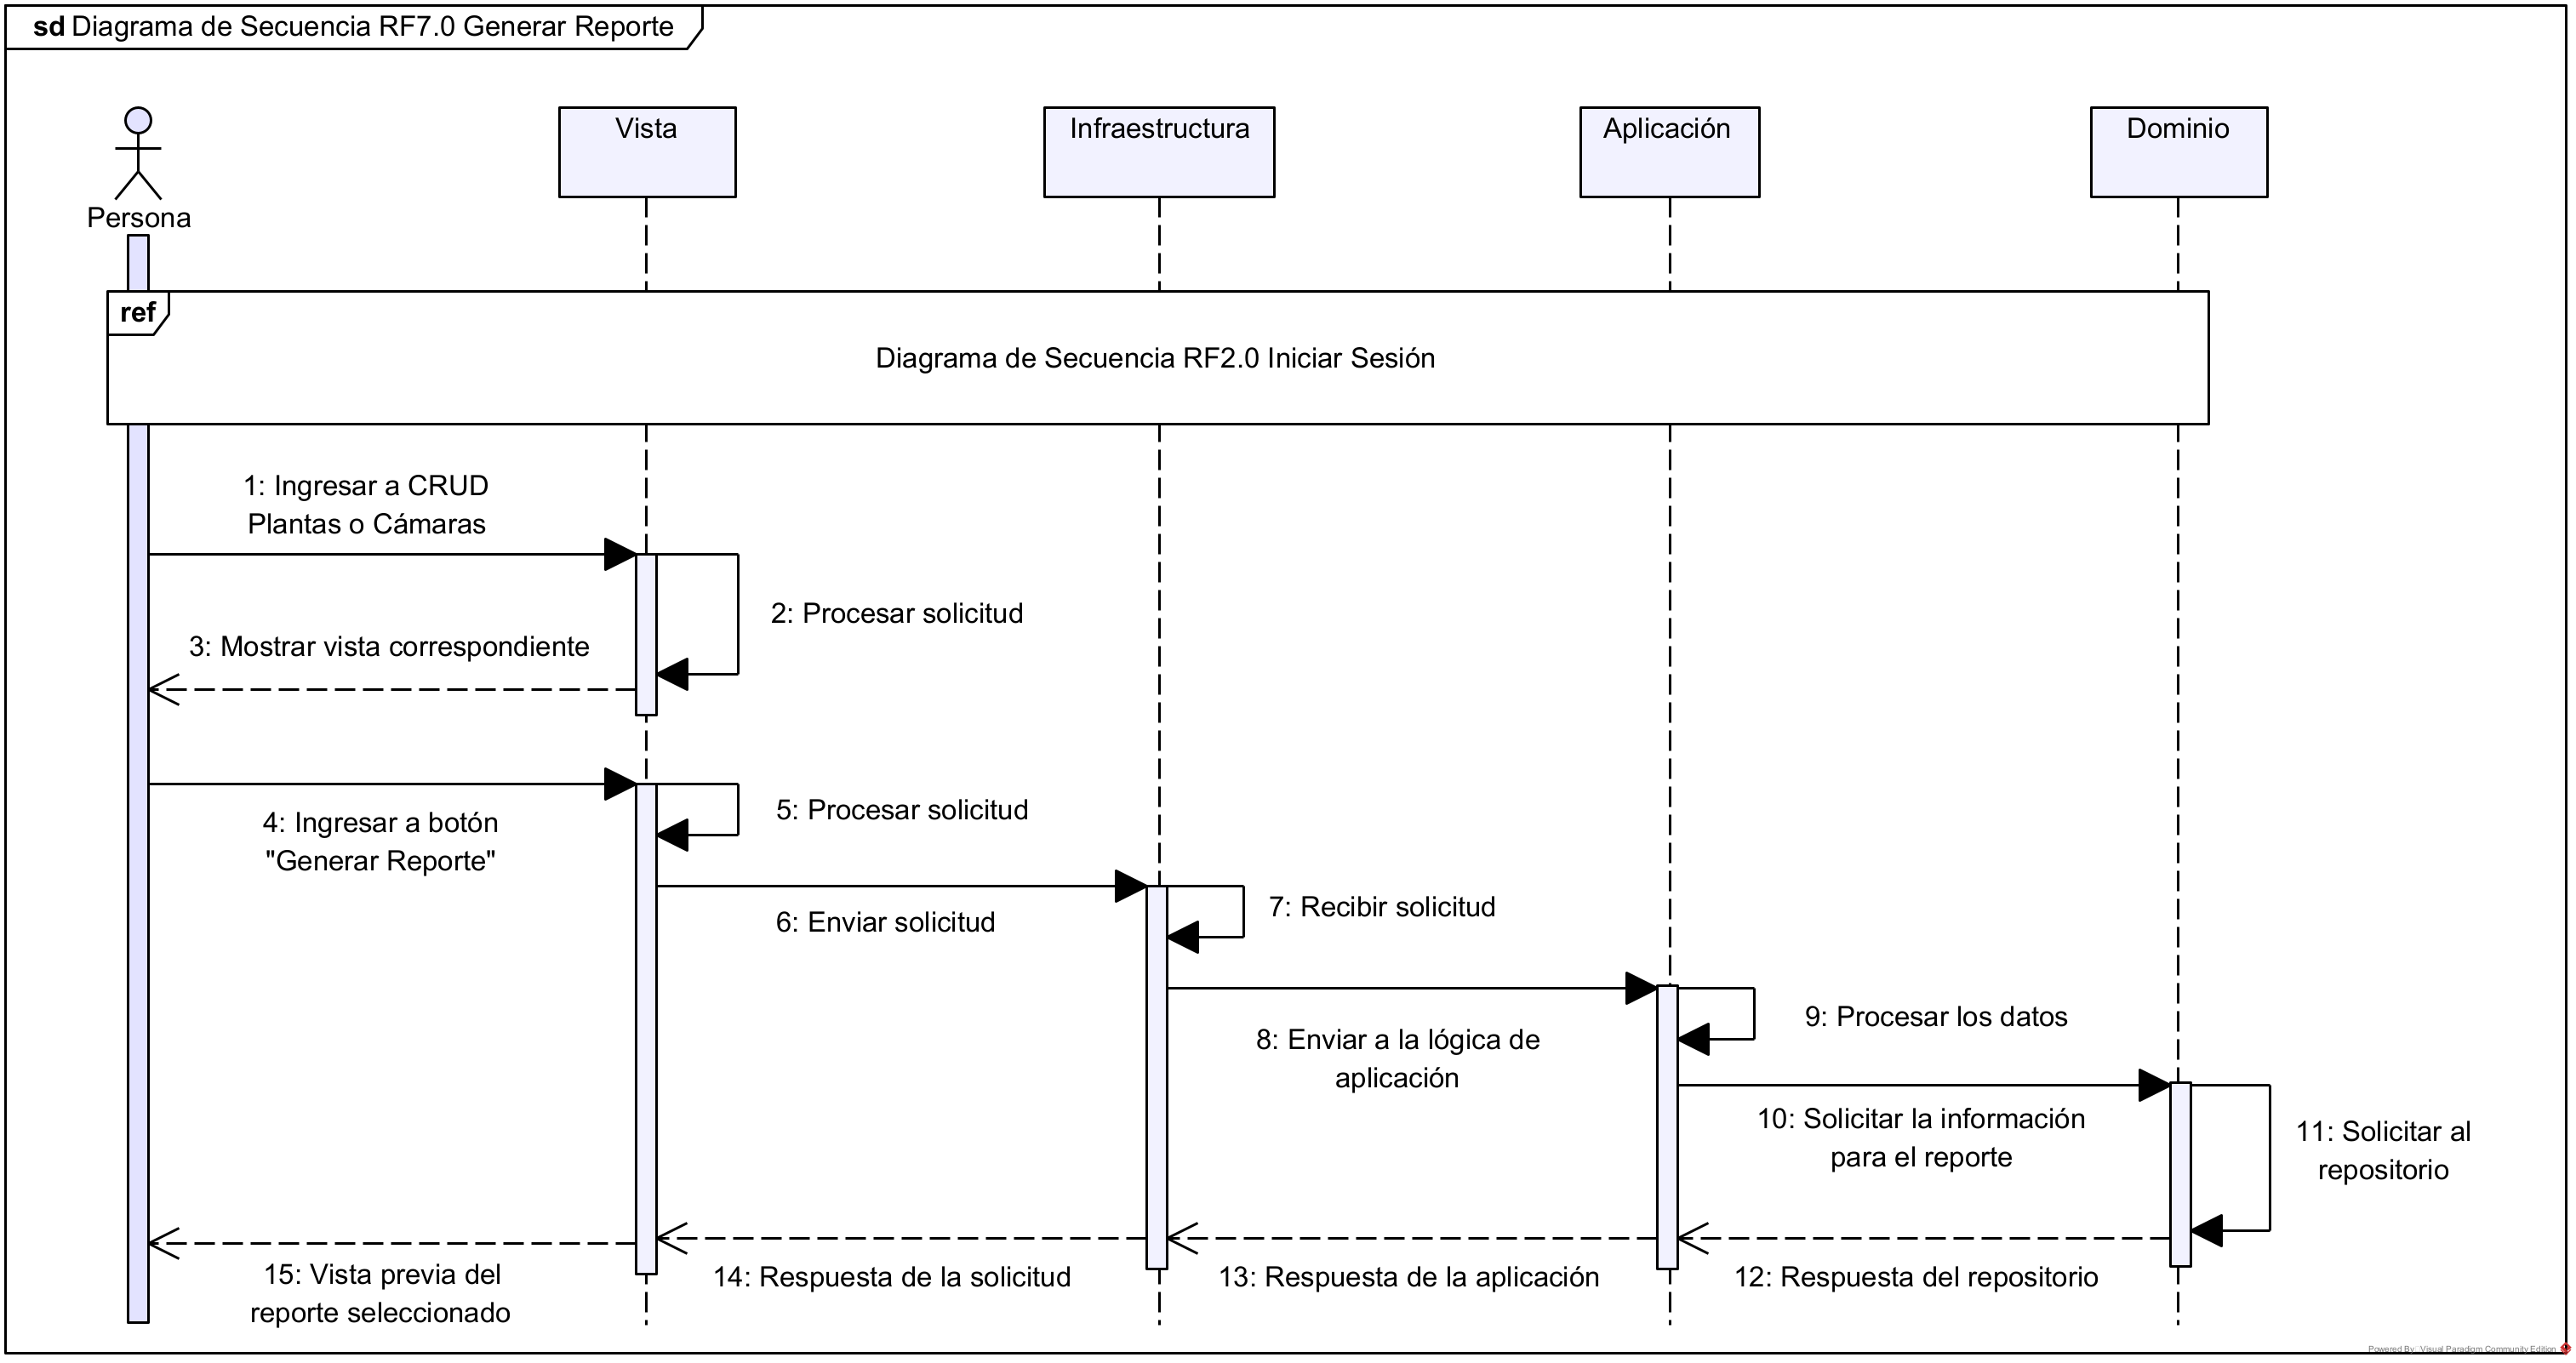
\includegraphics[width=0.8\textwidth]{UML/Secuencia/Diagrama de Secuencia RF7.0 Generar Reporte.png}
\end{figure}


\begin{figure}[H]
	\centering
	\caption{Diagrama de Secuencia para Descargar Reporte (RF7.1).}
 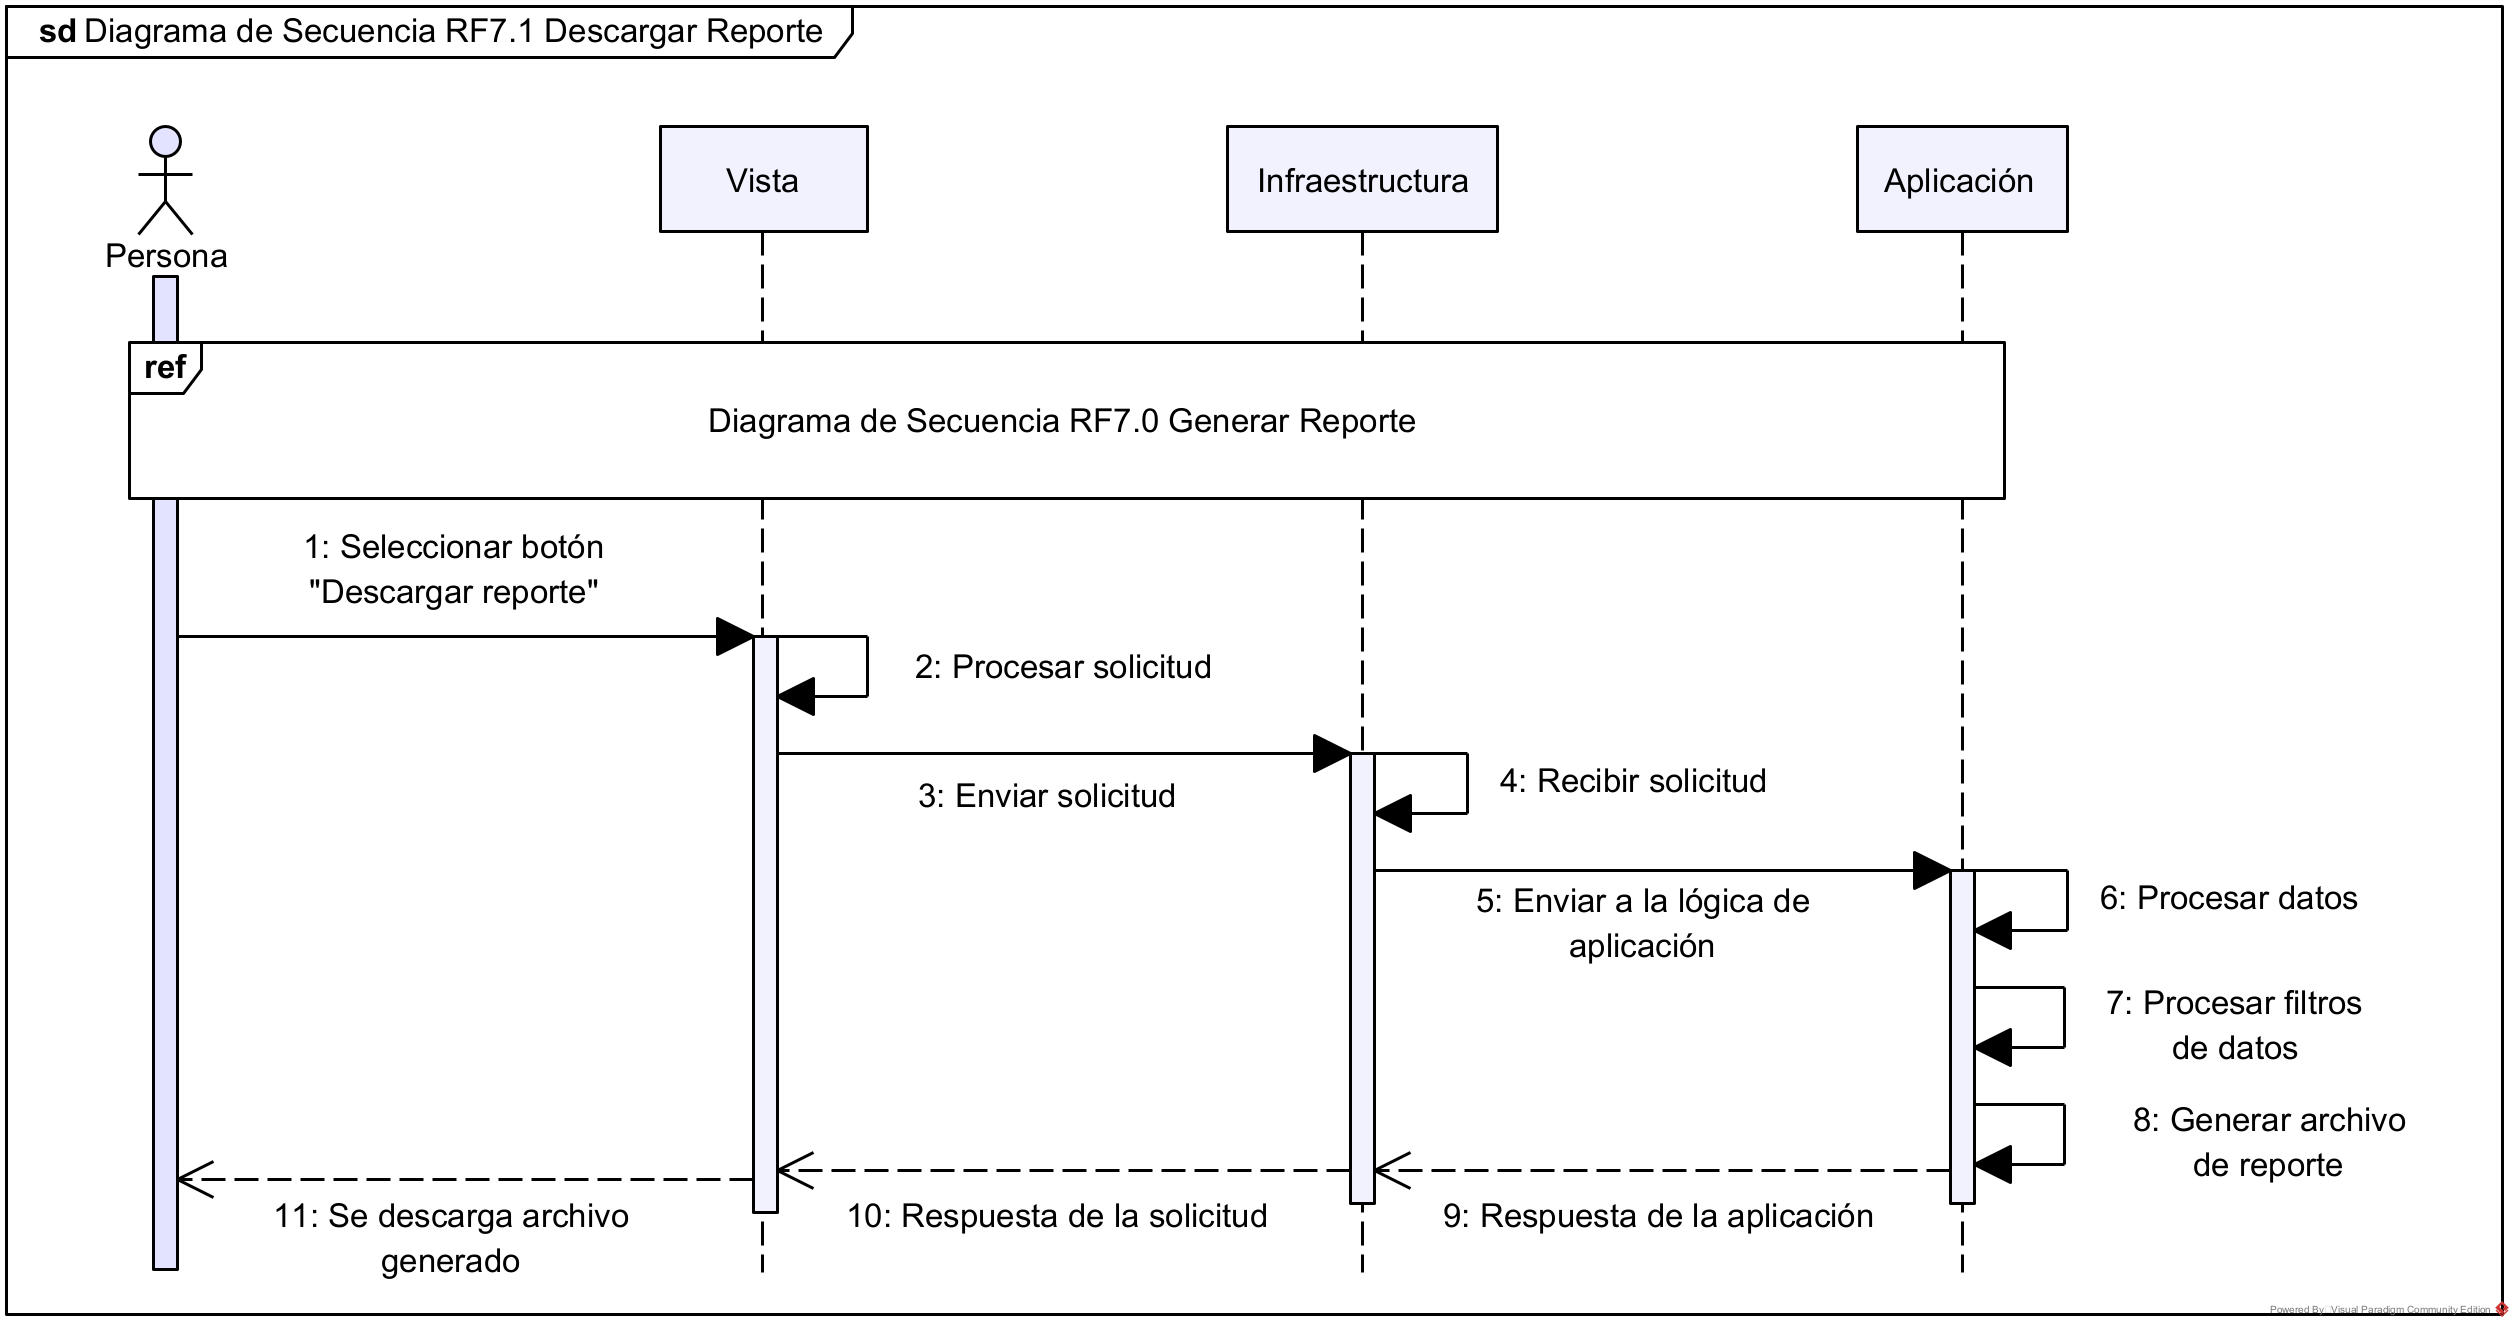
\includegraphics[width=0.8\textwidth]{UML/Secuencia/Diagrama de Secuencia RF7.1 Descargar Reporte.png}
\end{figure}


\begin{figure}[H]
	\centering
		\caption{Diagrama de Secuencia para Adjuntar Reporte (RF7.2).}
	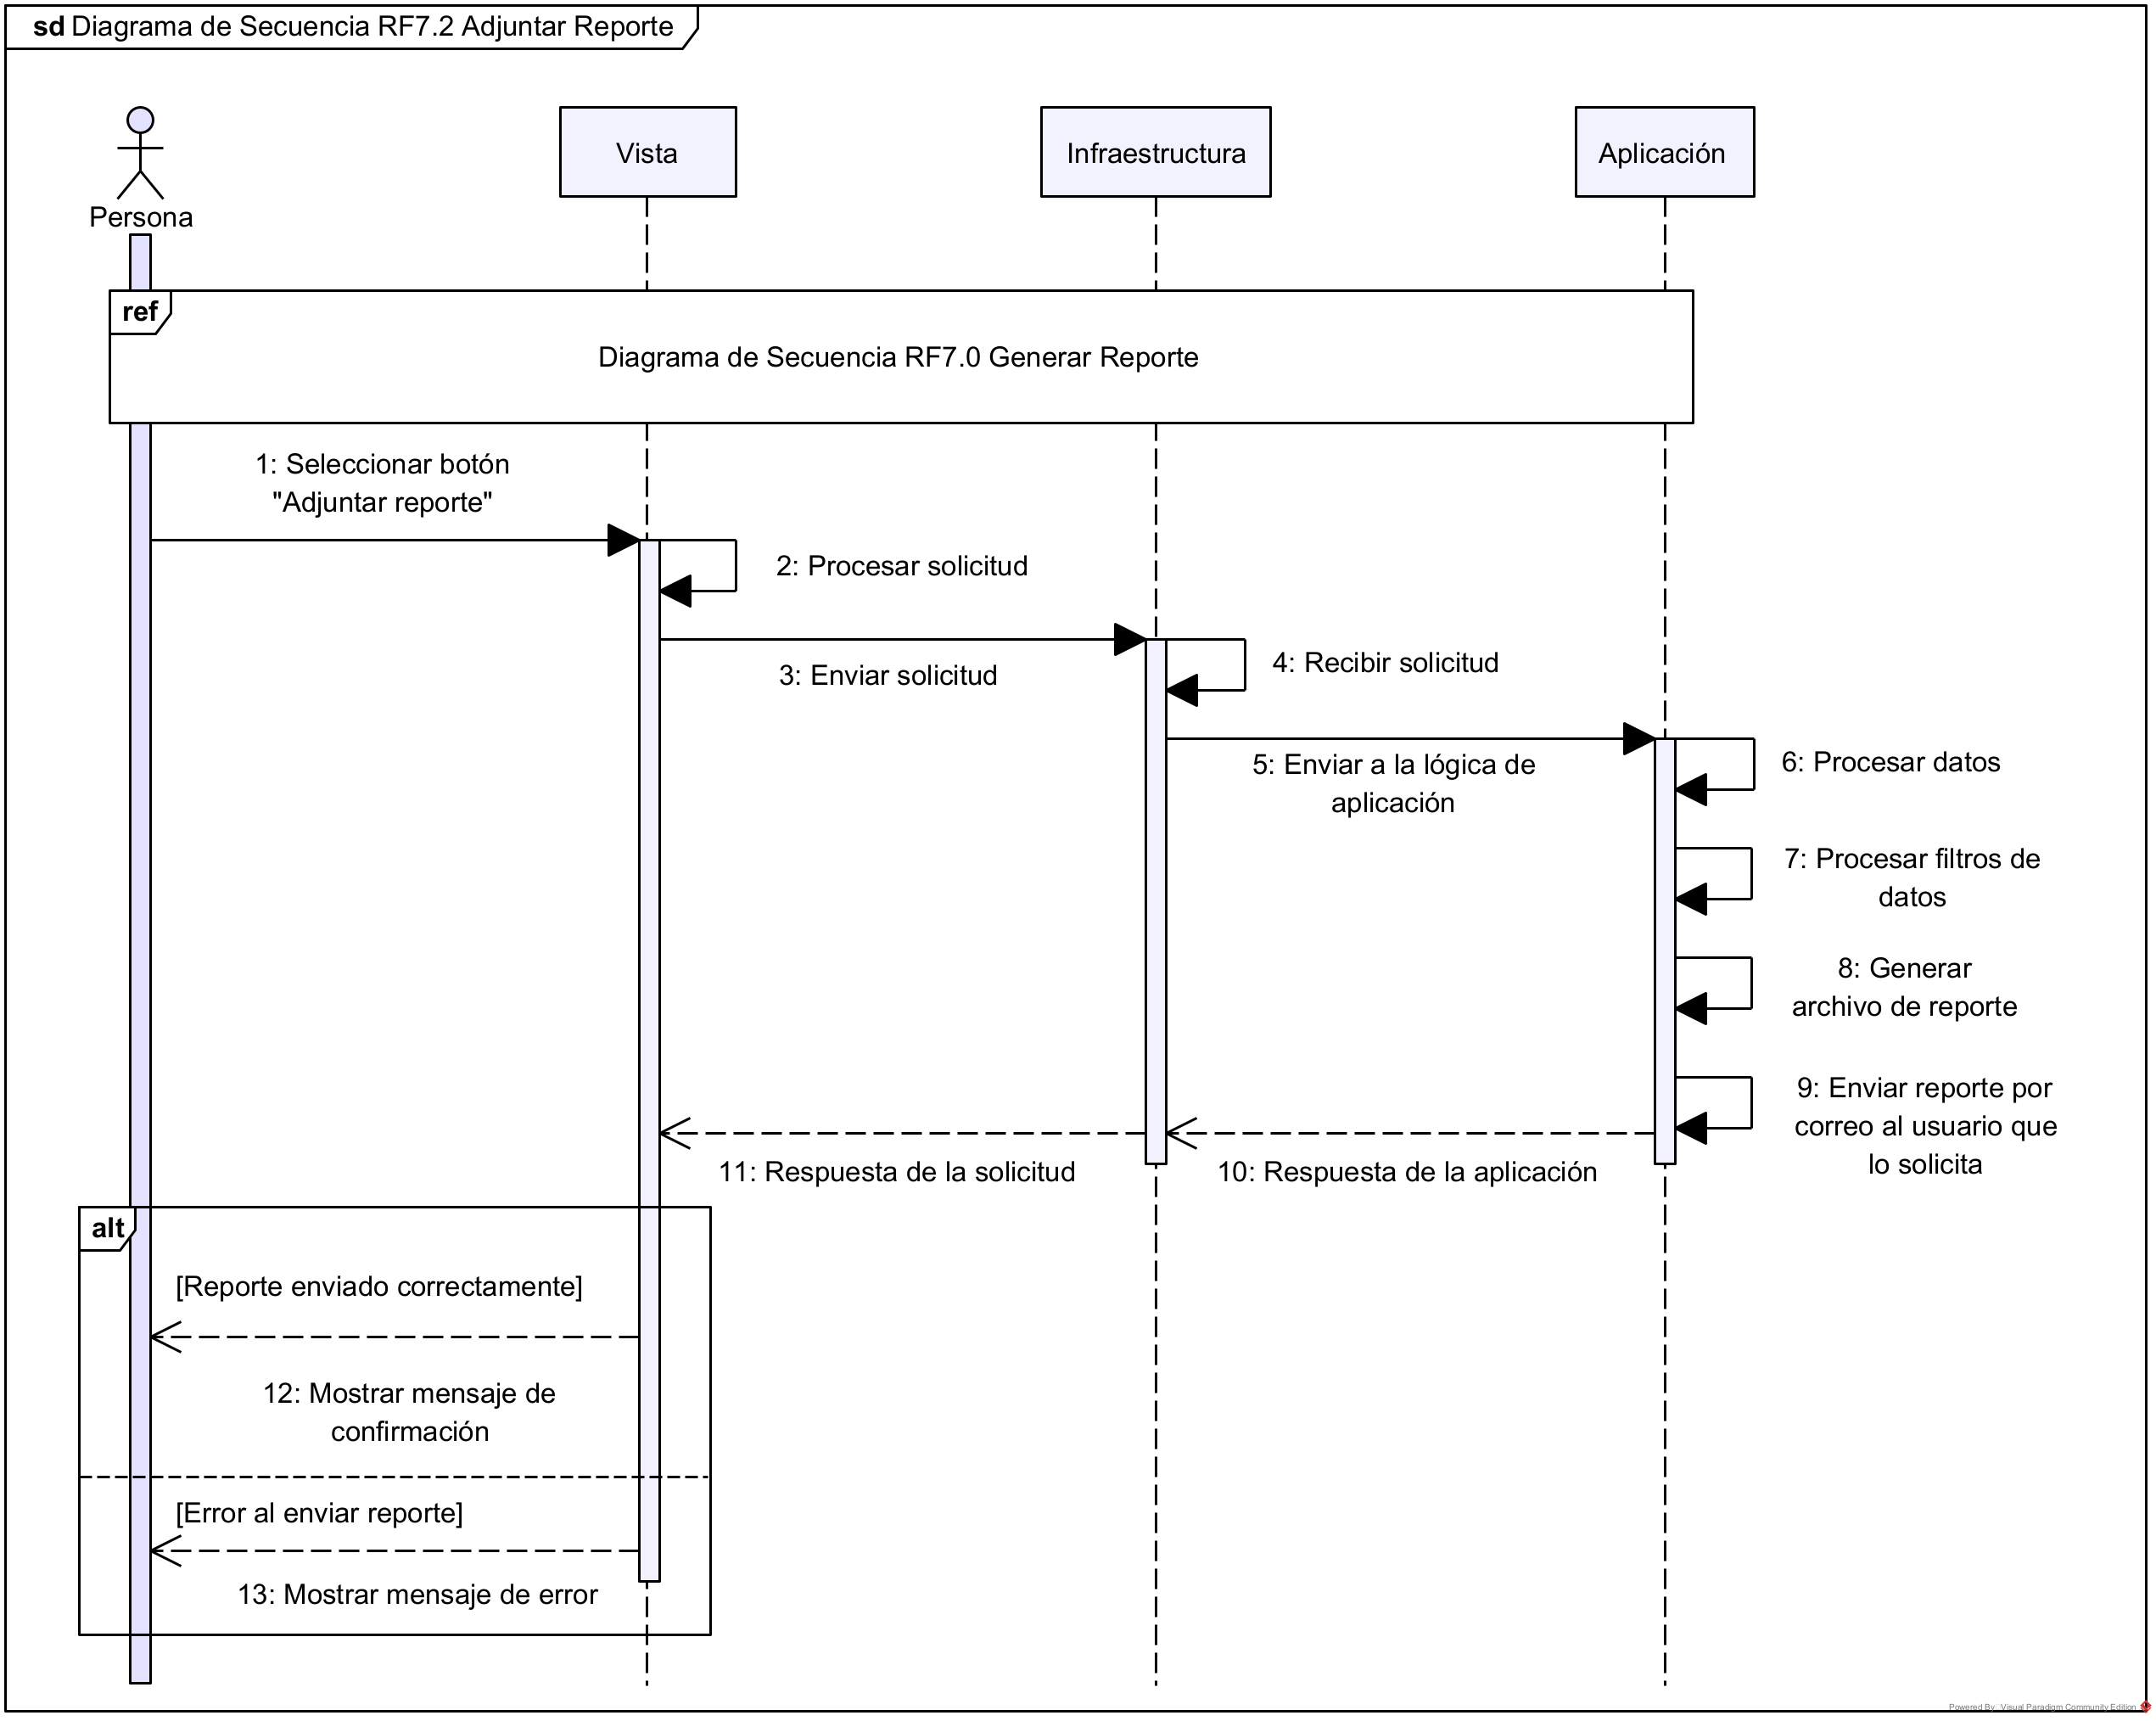
\includegraphics[width=0.8\textwidth]{UML/Secuencia/Diagrama de Secuencia RF7.2 Adjuntar Reporte.png}
\end{figure}


\begin{figure}[H]
	\centering
	\caption{Diagrama de Secuencia para Notificar Planta (RF8.1).}
 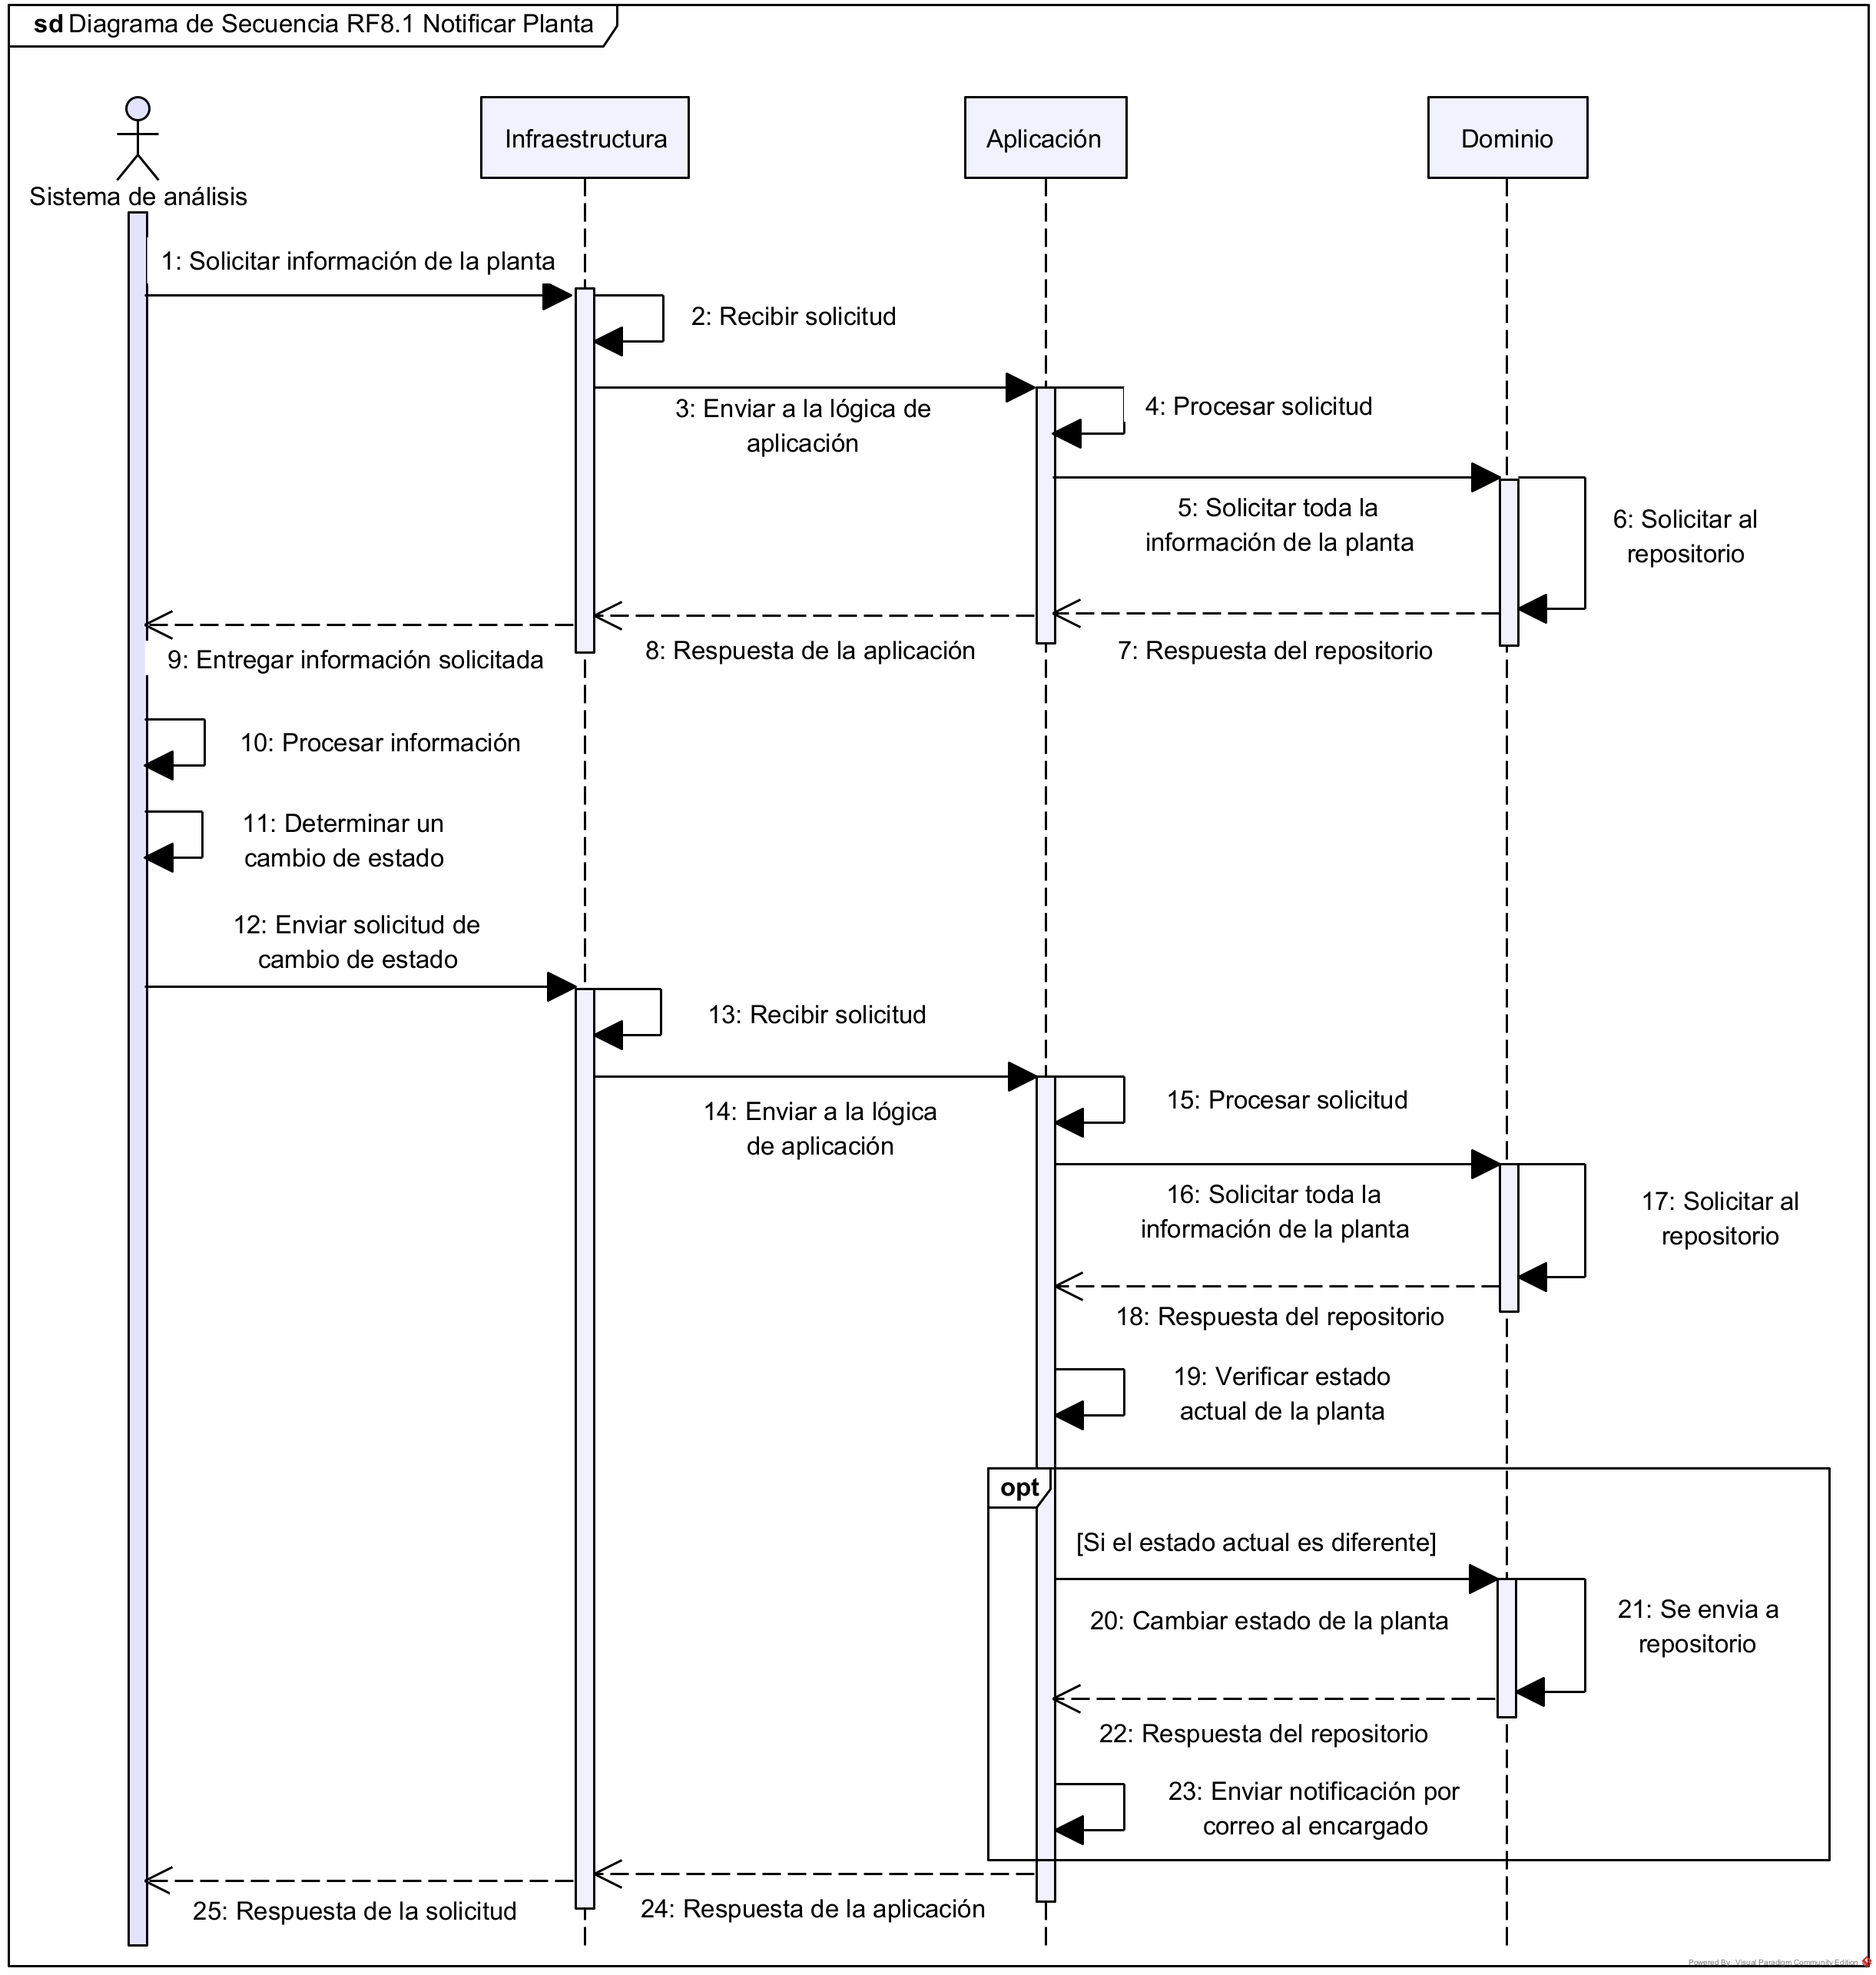
\includegraphics[width=0.8\textwidth]{UML/Secuencia/Diagrama de Secuencia RF8.1 Notificar Planta.png}
\end{figure}


\begin{figure}[H]
	\centering
	\caption{Diagrama de Secuencia para Notificar Seguridad (RF8.2).}
 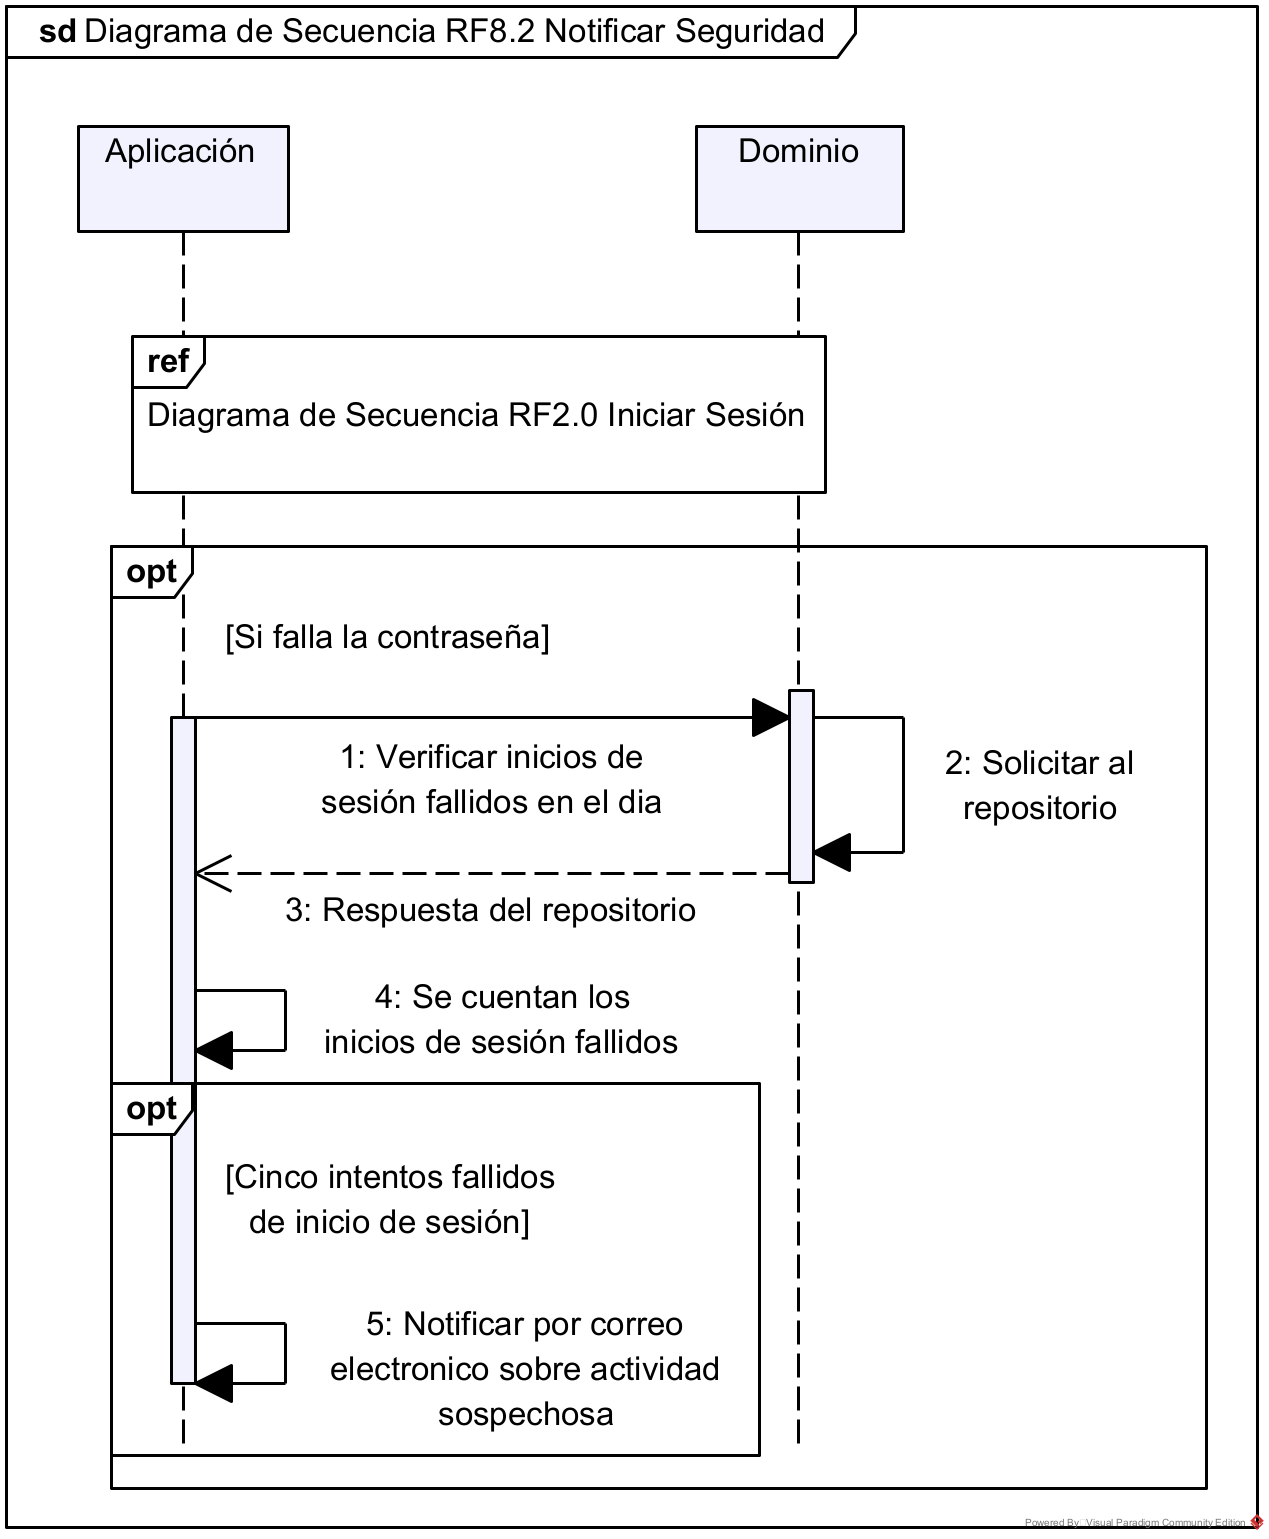
\includegraphics[width=0.8\textwidth]{UML/Secuencia/Diagrama de Secuencia RF8.2 Notificar Seguridad.png}
\end{figure}


\begin{figure}[H]
	\centering
	\caption{Diagrama de Secuencia para Crear Observación (RF9.1).}
 \includegraphics[width=0.8\textwidth]{UML/Secuencia/Diagrama de Secuencia RF9.1 Crear Observación.png}
\end{figure}


\begin{figure}[H]
	\centering
	\caption{Diagrama de Secuencia para Consultar Observación (RF9.1).}
 \includegraphics[width=0.8\textwidth]{UML/Secuencia/Diagrama de Secuencia RF9.2 Consultar Observación.png}
\end{figure}

% =================================================
% =================================================

\subsection{Diagramas de Actividades}

\begin{figure}[H]
    \centering
    \caption{Diagrama de Actividad para el Registro (RF1.0).}
    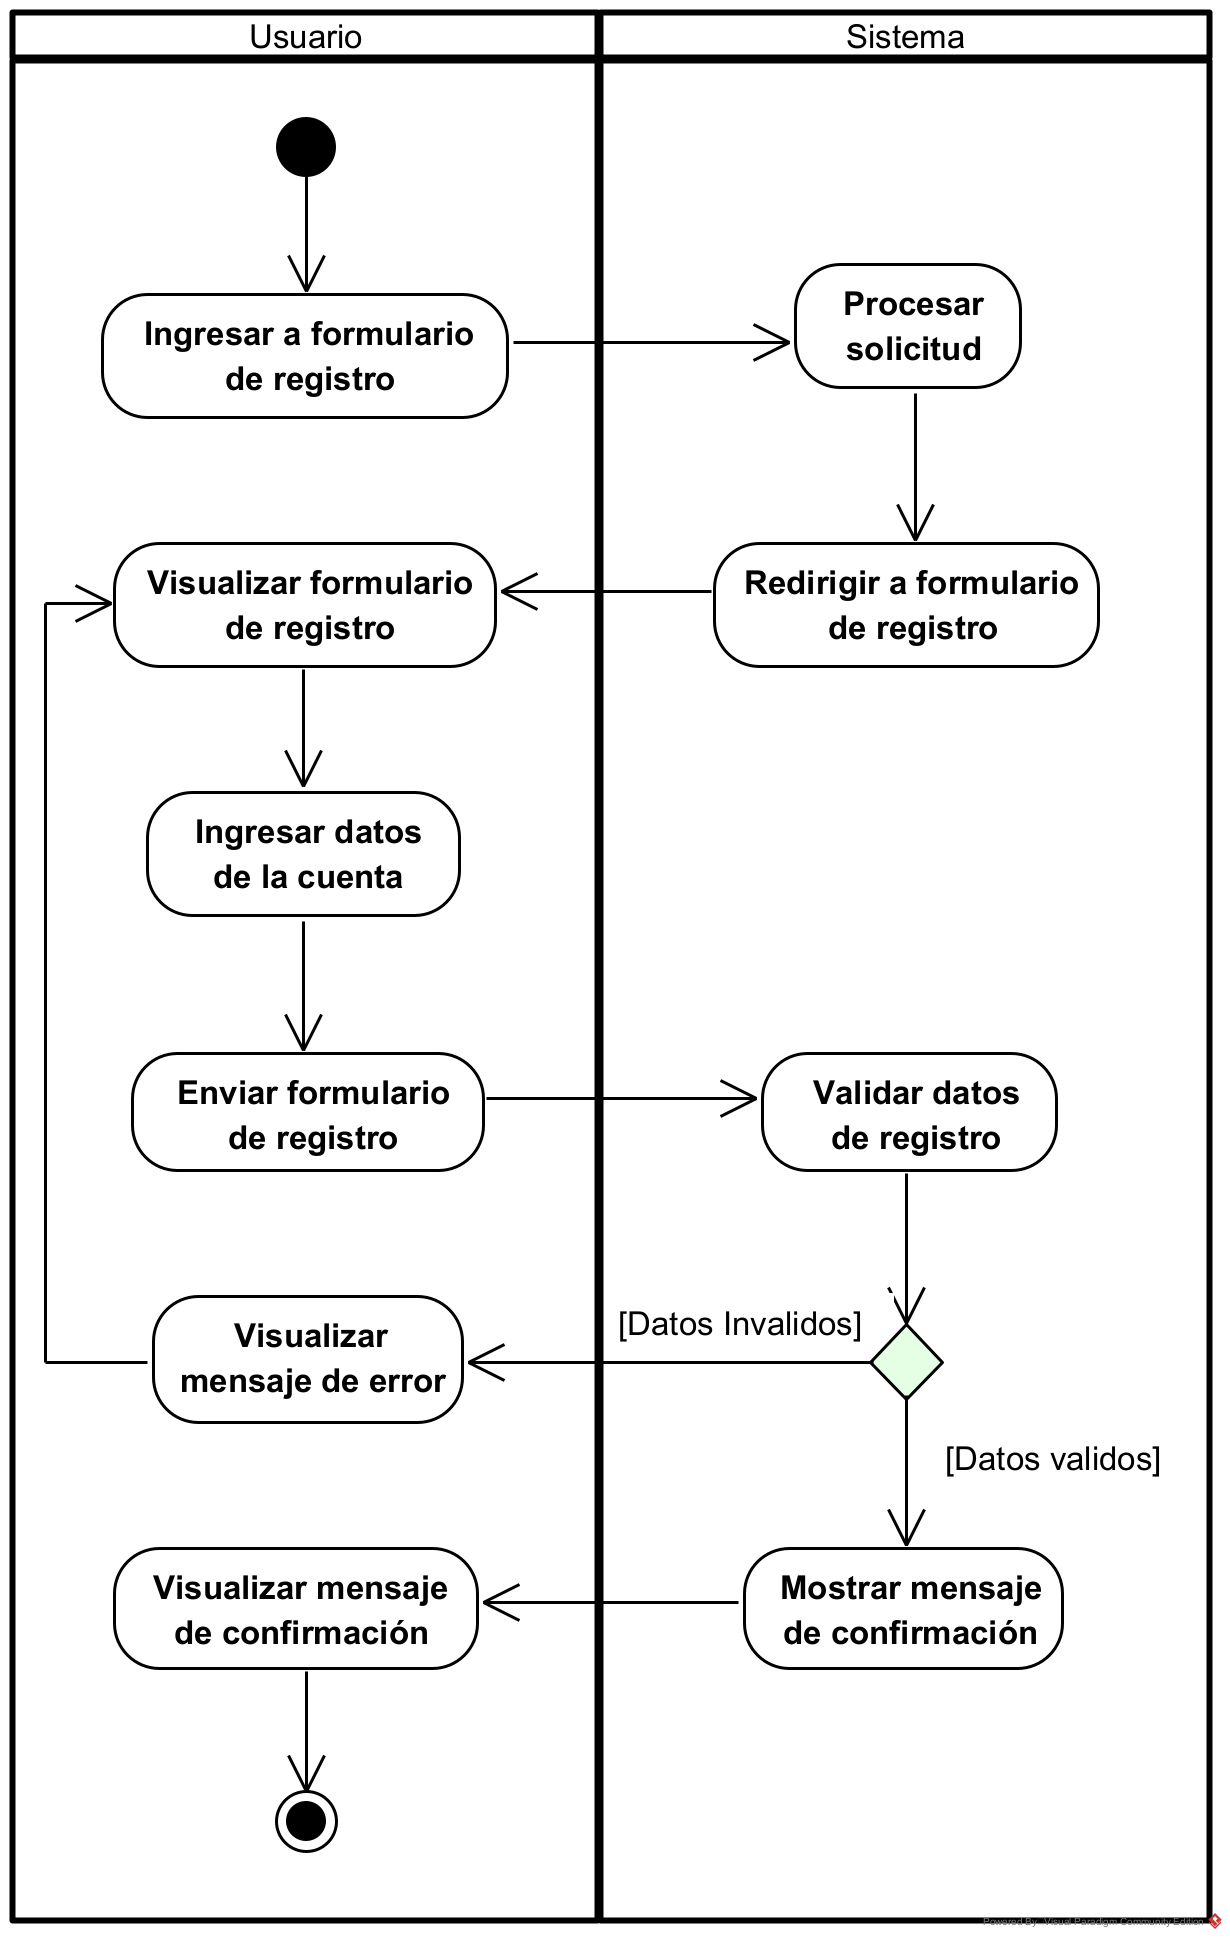
\includegraphics[width=0.7\textwidth]{UML/Actividad/Diagrama de Actividad RF1.0 Registro.png}
\end{figure}


\begin{figure}[H]
    \centering
    \caption{Diagrama de Actividad para Solicitar Código (RF1.1).}
 \includegraphics[width=0.6\textwidth]{UML/Actividad/Diagrama de Actividad RF1.1 Solicitar Código.png}
\end{figure}


\begin{figure}[H]
	\centering
	\caption{Diagrama de Actividad para Iniciar Sesión (RF2.0).}
 \includegraphics[width=0.7\textwidth]{UML/Actividad/Diagrama de Actividad RF2.0 Iniciar Sesión.png}
\end{figure}


\begin{figure}[H]
	\centering
		\caption{Diagrama de Actividad para Cerrar Sesión (RF2.1).}
	\includegraphics[width=0.65\textwidth]{UML/Actividad/Diagrama de Actividad RF2.1 Cerrar Sesión.png}
\end{figure}


\begin{figure}[H]
	\centering
	\caption{Diagrama de Actividad para Recuperar Contraseña (RF2.2).}
 \includegraphics[width=0.8\textwidth]{UML/Actividad/Diagrama de Actividad RF2.2 Recuperar Contraseña.png}
\end{figure}


\begin{figure}[H]
	\centering
	\caption{Diagrama de Actividad para Crear Cámara (RF3.1).}
 \includegraphics[width=0.8\textwidth]{UML/Actividad/Diagrama de Actividad RF3.1 Crear Cámara.png}
\end{figure}


\begin{figure}[H]
	\centering
		\caption{Diagrama de Actividad para Activar Cámara (RF3.1.1).}
	\includegraphics[width=0.8\textwidth]{UML/Actividad/Diagrama de Actividad RF3.1.1 Activar Cámara.png}
\end{figure}


\begin{figure}[H]
	\centering
		\caption{Diagrama de Actividad para Activar Hardware (RF3.1.1).}
	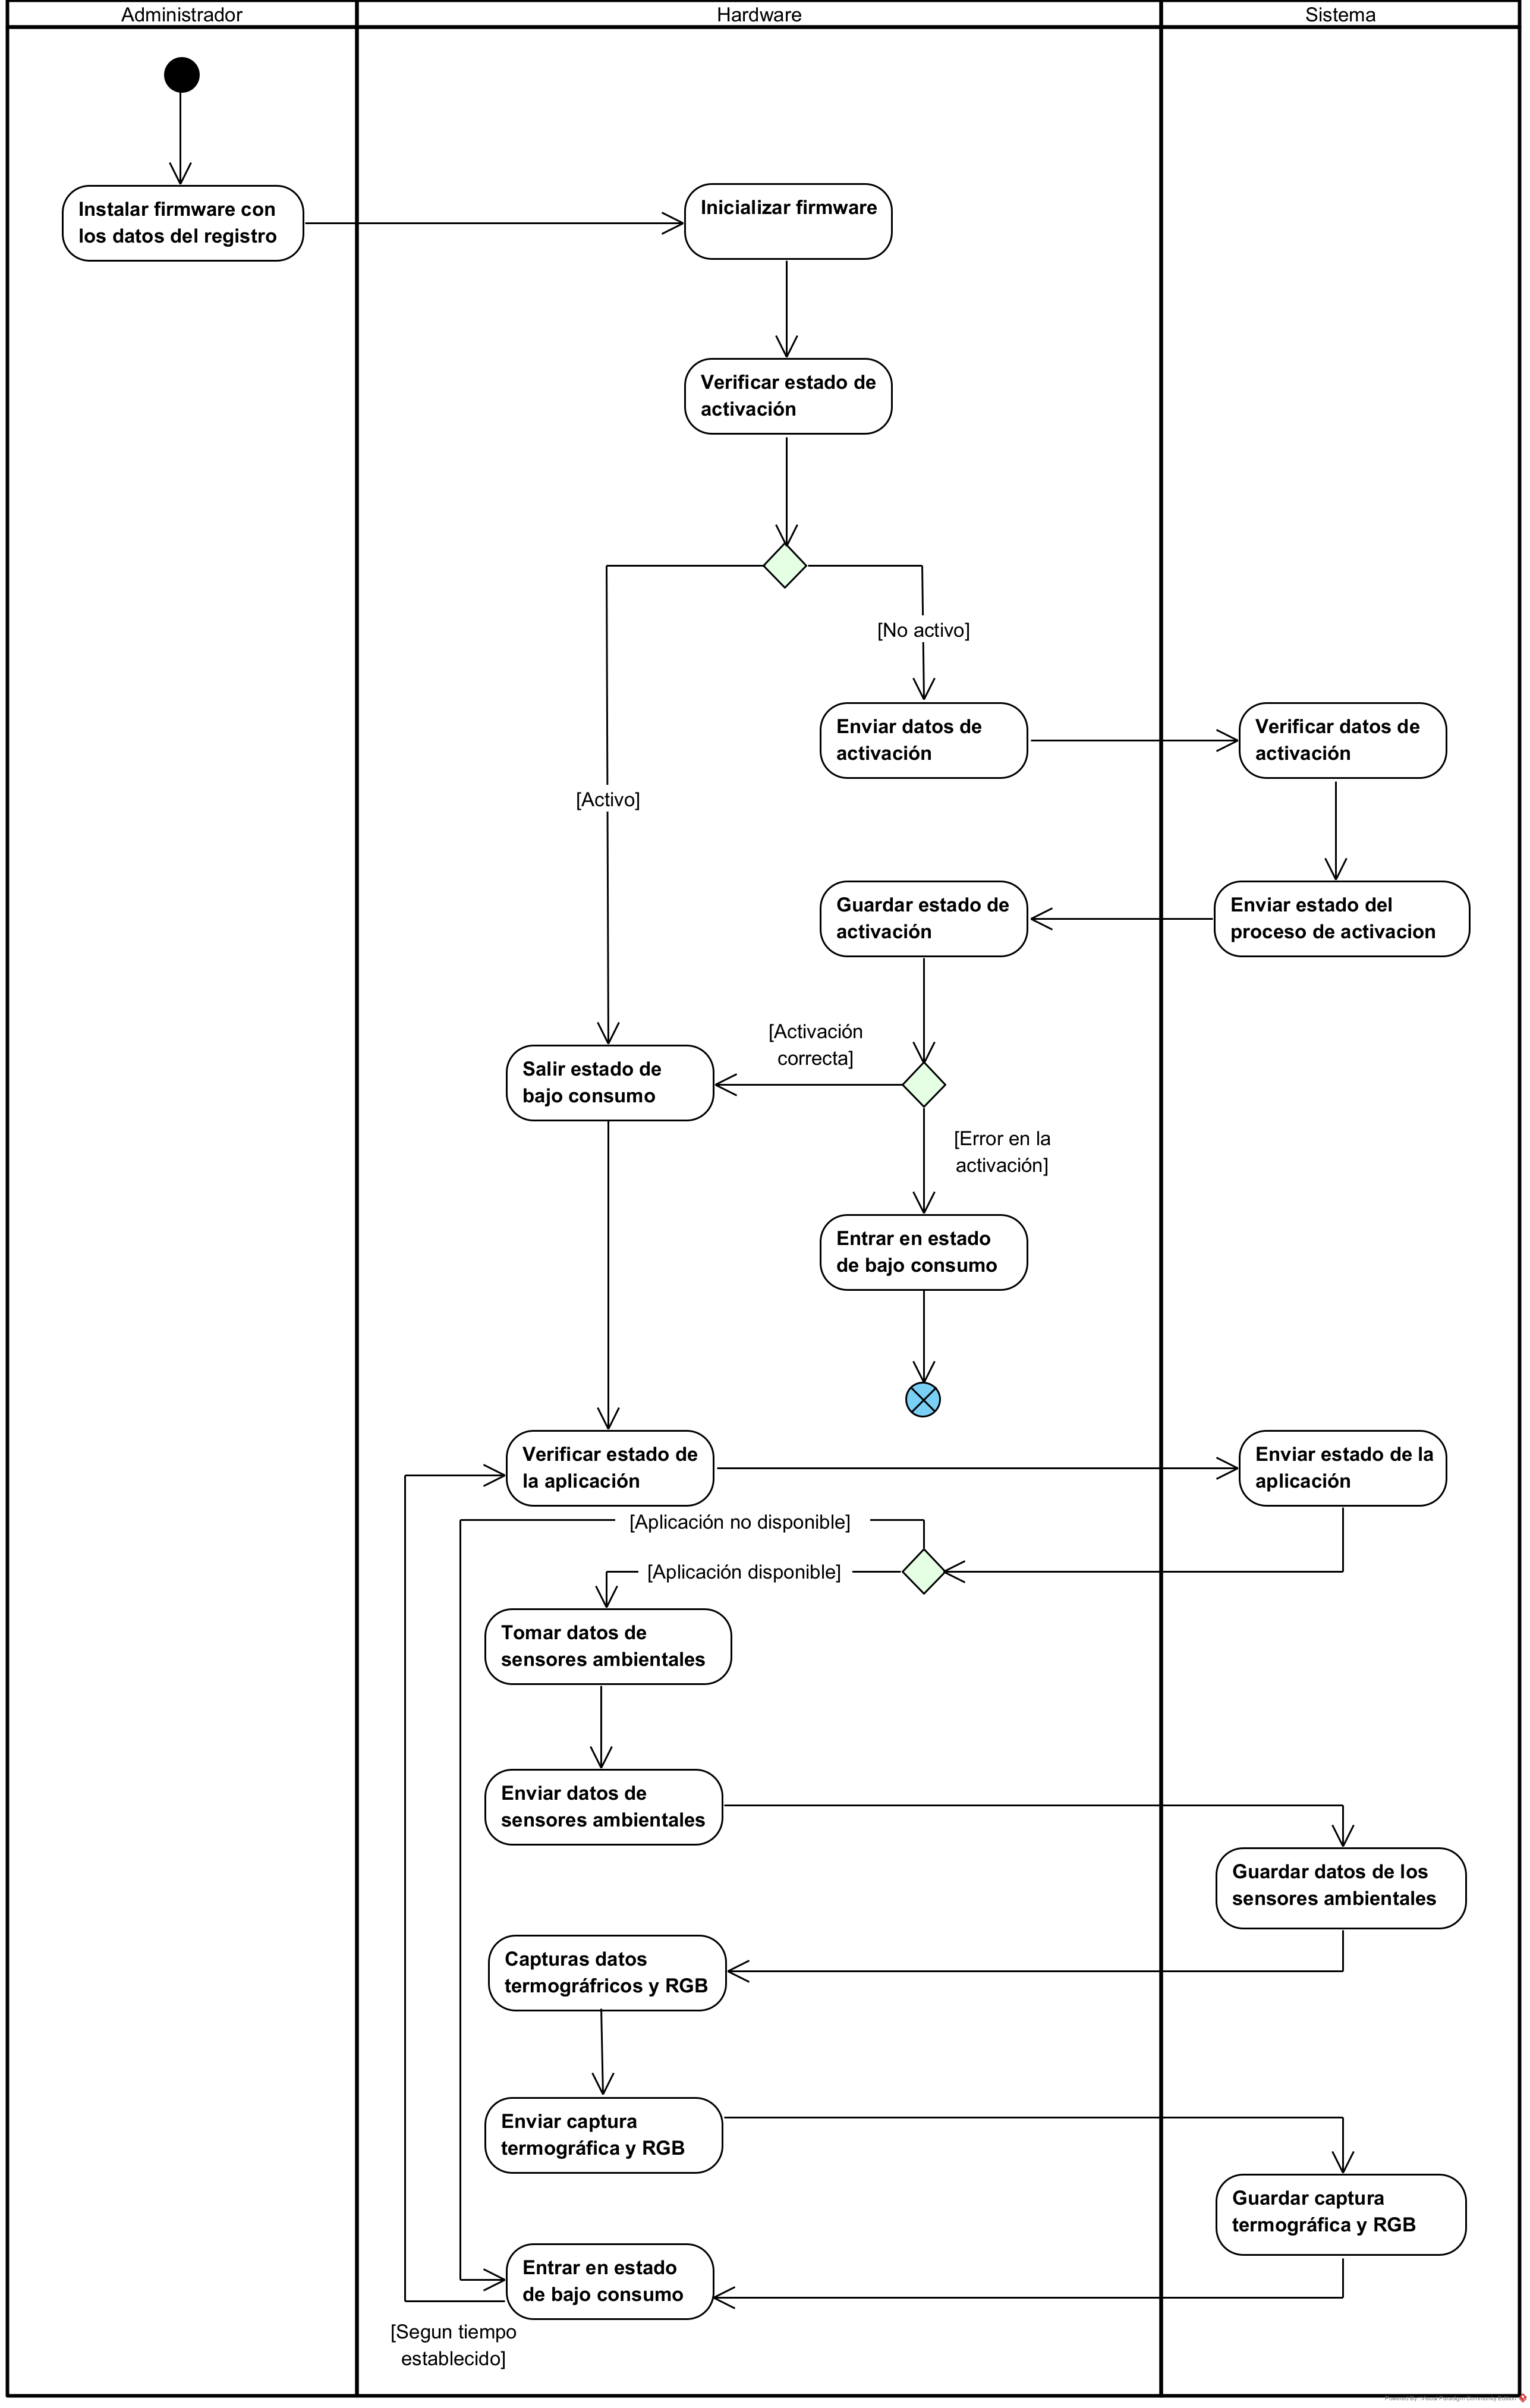
\includegraphics[width=0.8\textwidth]{UML/Actividad/Diagrama de Actividad RF3.1.1 Activar Hardware.png}
\end{figure}


\begin{figure}[H]
	\centering
	\caption{Diagrama de Actividad para Consultar Cámara (RF3.2).}
 \includegraphics[width=0.8\textwidth]{UML/Actividad/Diagrama de Actividad RF3.2 Consultar Cámara.png}
\end{figure}


\begin{figure}[H]
	\centering
	\caption{Diagrama de Actividad para Editar Cámara (RF3.3).}
 \includegraphics[width=0.8\textwidth]{UML/Actividad/Diagrama de Actividad RF3.3 Editar Cámara.png}
\end{figure}


\begin{figure}[H]
	\centering
		\caption{Diagrama de Actividad para Eliminar Cámara (RF3.4).}
\includegraphics[width=0.8\textwidth]{UML/Actividad/Diagrama de Actividad RF3.4 Eliminar Cámara.png}
\end{figure}


\begin{figure}[H]
	\centering
		\caption{Diagrama de Actividad para Consultar Perfil (RF4.1).}
	\includegraphics[width=0.8\textwidth]{UML/Actividad/Diagrama de Actividad RF4.1 Consultar Perfil.png}
\end{figure}


\begin{figure}[H]
	\centering
	\caption{Diagrama de Actividad para Editar Perfil (RF4.2).}
 \includegraphics[width=0.8\textwidth]{UML/Actividad/Diagrama de Actividad RF4.2 Editar Perfil.png}
\end{figure}


\begin{figure}[H]
	\centering
	\caption{Diagrama de Actividad para Eliminar Perfil (RF4.3).}
 \includegraphics[width=0.8\textwidth]{UML/Actividad/Diagrama de Actividad RF4.3 Eliminar Perfil.png}
\end{figure}


\begin{figure}[H]
	\centering
		\caption{Diagrama de Actividad para Cambiar Contraseña (RF4.4).}
	\includegraphics[width=0.8\textwidth]{UML/Actividad/Diagrama de Actividad RF4.4 Cambiar Contraseña.png}
\end{figure}


\begin{figure}[H]
	\centering
	\caption{Diagrama de Actividad para Agregar Integrante de Cultivo (RF4.5).}
 \includegraphics[width=0.8\textwidth]{UML/Actividad/Diagrama de Actividad RF4.5 Agregar Integrante Cultivo.png}
\end{figure}


\begin{figure}[H]
	\centering
	\caption{Diagrama de Actividad para Eliminar Integrante de Cultivo (RF4.6).}
 \includegraphics[width=0.8\textwidth]{UML/Actividad/Diagrama de Actividad RF4.6 Eliminar Integrante Cultivo.png}
\end{figure}

\begin{figure}[H]
	\centering
	\caption{Diagrama de Actividad para el Módulo de Mediciones (RF5.0).}
 \includegraphics[width=0.8\textwidth]{UML/Actividad/Diagrama de Actividad RF5.0 Módulo de mediciones.png}
\end{figure}


\begin{figure}[H]
	\centering
	\caption{Diagrama de Actividad para Crear Planta (RF6.1).}
 \includegraphics[width=0.8\textwidth]{UML/Actividad/Diagrama de Actividad RF6.1 Crear Planta.png}
\end{figure}


\begin{figure}[H]
	\centering
	\caption{Diagrama de Actividad para Consultar Planta (RF6.2).}
 \includegraphics[width=0.8\textwidth]{UML/Actividad/Diagrama de Actividad RF6.2 Consultar Planta.png}
\end{figure}


\begin{figure}[H]
	\centering
		\caption{Diagrama de Actividad para Editar Planta (RF6.3).}
	\includegraphics[width=0.8\textwidth]{UML/Actividad/Diagrama de Actividad RF6.3 Editar Planta.png}
\end{figure}


\begin{figure}[H]
	\centering
	\caption{Diagrama de Actividad para Eliminar Planta (RF6.4).}
 \includegraphics[width=0.8\textwidth]{UML/Actividad/Diagrama de Actividad RF6.4 Eliminar Planta.png}
\end{figure}


\begin{figure}[H]
	\centering
		\caption{Diagrama de Actividad para Generar Reporte (RF7.0).}
	\includegraphics[width=0.8\textwidth]{UML/Actividad/Diagrama de Actividad RF7.0 Generar Reporte.png}
\end{figure}


\begin{figure}[H]
	\centering
		\caption{Diagrama de Actividad para Descargar Reporte (RF7.1).}
\includegraphics[width=0.8\textwidth]{UML/Actividad/Diagrama de Actividad RF7.1 Descargar Reporte.png}
\end{figure}


\begin{figure}[H]
	\centering
		\caption{Diagrama de Actividad para Adjuntar Reporte (RF7.2).}
\includegraphics[width=0.8\textwidth]{UML/Actividad/Diagrama de Actividad RF7.2 Adjuntar Reporte.png}
\end{figure}


\begin{figure}[H]
	\centering
	\caption{Diagrama de Actividad para Notificar Planta (RF8.1).}
 \includegraphics[width=0.8\textwidth]{UML/Actividad/Diagrama de Actividad RF8.1 Notificar Planta.png}
\end{figure}


\begin{figure}[H]
	\centering
		\caption{Diagrama de Actividad para Notificar Seguridad (RF8.2).}
	\includegraphics[width=0.8\textwidth]{UML/Actividad/Diagrama de Actividad RF8.2 Notificar Seguridad.png}
\end{figure}


\begin{figure}[H]
	\centering
	\caption{Diagrama de Actividad para Crear Observación (RF9.1).}
 \includegraphics[width=0.8\textwidth]{UML/Actividad/Diagrama de Actividad RF9.1 Crear Observación.png}
\end{figure}


\begin{figure}[H]
	\centering
		\caption{Diagrama de Actividad para Consultar Observación (RF9.2).}
	\includegraphics[width=0.8\textwidth]{UML/Actividad/Diagrama de Actividad RF9.2 Consultar Observación.png}
\end{figure}

% =================================================
% =================================================

\subsection{Diagrama de Clases}
Incluir el diagrama con descripciones por cada clase.

% =================================================
% =================================================

\subsection{Diagrama de Despliegue}
\begin{figure}[H]
    \centering
    \caption{Diagrama de Despliegue del Sistema.}
    \label{fig:despliegue}
    \includegraphics[width=0.8\textwidth]{UML/Otros/Diagrama de Despliegue.png}
\end{figure}

% =================================================
% =================================================

\section{Diseño de los Casos de Prueba}
Texto sobre el diseño de casos de prueba utilizando SonarQube.

% =================================================
% =================================================

\section{Estimación de Recursos}
Texto sobre la estimación de recursos utilizando el método de puntos de función o puntos de casos de uso.

\section{Resultados de la Implementación del Software}
Texto sobre el resultado de implementar el software.

\section{Conclusiones y Recomendaciones del software}
Discusión, conclusiones y recomendaciones sobre el software y su integración.
